% !TEX root = ./notes_template.tex
%%%%%%%%%%%%%%%%%%%%%%%%%%%%%%%%%%%%%%%%%%%%%%%%%%
%%%%%%%%%%%%%%%%%%%%% preamble %%%%%%%%%%%%%%%%%%%
%%%%%%%%%%%%%%%%%%%%%%%%%%%%%%%%%%%%%%%%%%%%%%%%%%
%\documentclass[11pt,twoside]{book}
%=== [salt] 12p로 변경함 - 작업했던 폰트
%\documentclass[12pt,twoside]{book}

%== [salt] 아래 클래스는 잘 안됨
%\documentclass{oblivoir}
%\usepackage[dbl4x6]{fapapersize}

\documentclass[10.5pt,twoside]{book}

\usepackage[mono=false]{libertine} % new linux font, ignore mono

%=== [salt] 한글 tex 을 위한 패키지 추가 ===
\usepackage{kotex}

\usepackage{luatex85}

%==[salt] 수식에서 지워지는 항 표시하기
\usepackage{cancel}  


\usepackage{amsmath,amsthm,amssymb,mathrsfs,amsfonts,dsfont}
\usepackage{epsfig,graphicx}
\usepackage{tabularx}
\usepackage{blkarray}
\usepackage{slashed}
\usepackage{color}
\usepackage{listings}
\usepackage{caption}
% \usepackage{fullpage}
\usepackage{lipsum} % provides dummy text for testing
\usepackage[toc,title,titletoc,header]{appendix}
\usepackage{minitoc}
\usepackage{color}
\usepackage{multicol} % two-col ToC
\usepackage{multirow} % ===[salt]
\usepackage{bm}
\usepackage{imakeidx} % before hyperref
\usepackage{hyperref}
% link colors settings
\hypersetup{
    colorlinks=true,
    citecolor=magenta,
    linkcolor=blue,
    filecolor=green,      
    urlcolor=cyan,
    % hypertexnames=false,
}
\usepackage[capitalise]{cleveref}
\usepackage{subcaption}
\usepackage{enumitem}
\usepackage{mathtools}
\usepackage{physics}
\usepackage[linesnumbered,ruled,vlined,algosection]{algorithm2e}
\SetCommentSty{textsf}
\usepackage{epigraph}
\epigraphwidth=1.0\linewidth
\epigraphrule=0pt

% adjust margin
\usepackage[margin=2.3cm]{geometry}
\headheight13.6pt

%==============================
%=== [salt] 아래는 thmtools로 ``정리(Theorem)'' 스타일을 마음대로 만들때 사용함
%=== [salt] 관련 문서: thmtools-manual.pdf
%%%%%%%%%%%%%%%% thmtools %%%%%%%%%%%%%%%%%%%%%
\usepackage{thmtools}
\usepackage{layout}
\declaretheorem[numberwithin=chapter]{theorem}
\declaretheorem[numberwithin=chapter]{axiom}
\declaretheorem[numberwithin=chapter]{lemma}
\declaretheorem[numberwithin=chapter]{proposition}
\declaretheorem[numberwithin=chapter]{claim}
\declaretheorem[numberwithin=chapter]{conjecture}
\declaretheorem[sibling=theorem]{corollary}
\declaretheorem[numberwithin=chapter, style=definition]{definition}
\declaretheorem[numberwithin=chapter, style=definition]{problem}
\declaretheorem[numberwithin=chapter, style=definition]{example}
\declaretheorem[numberwithin=chapter, style=definition]{exercise}
\declaretheorem[numberwithin=chapter, style=definition]{observation}
\declaretheorem[numberwithin=chapter, style=definition]{fact}
\declaretheorem[numberwithin=chapter, style=definition]{construction}
\declaretheorem[numberwithin=chapter, style=definition]{remark}
\declaretheorem[numberwithin=chapter, style=remark]{question}
%==============================
\declaretheorem[numberwithin=chapter, style=definition, title=정리]{salt_theorem}
\declaretheorem[numberwithin=chapter, style=definition, title=보조정리]{salt_lemma}
\declaretheorem[numberwithin=chapter, style=definition, title=따름정리]{salt_corollary}
\declaretheorem[numberwithin=chapter, style=definition, title=정의]{salt_definition}
\declaretheorem[numberwithin=chapter, style=definition, title=예제]{salt_example}
\declaretheorem[numberwithin=chapter, style=definition, title=연습문제]{salt_exercise}
\declaretheorem[numberwithin=chapter, style=definition, title=명제]{salt_prop}
\declaretheorem[numberwithin=chapter, style=definition, title=참고]{salt_remark}
\declaretheorem[numberwithin=chapter, style=definition, title=추측]{salt_conjecture}
%%%%%%%%%%%%%%%% thmtools %%%%%%%%%%%%%%%%%%%%%
%==============================
%=== [salt] 수식번호 넣는 법
%\numberwithin{equation}{section}
\numberwithin{equation}{chapter}
\numberwithin{figure}{chapter}

\usepackage{changepage}
\newenvironment{solution}
    {\renewcommand\qedsymbol{$\square$}\color{blue}\begin{adjustwidth}{0em}{2em}\begin{proof}[\textit Solution.~]}
    {\end{proof}\end{adjustwidth}}

%%%%%%%%%%%%%%%% index %%%%%%%%%%%%%%%%%%%%%
\begin{filecontents}{index.ist}
% https://tex.stackexchange.com/questions/65247/index-with-an-initial-letter-of-the-group
headings_flag 1
heading_prefix "{\\centering\\large \\textbf{"
heading_suffix "}}\\nopagebreak\n"
delim_0 "\\nobreak\\dotfill"
\end{filecontents}
\newcommand{\myindex}[1]{\index{#1} \emph{#1}}
\makeindex[columns=3, intoc, title=Alphabetical Index, options= -s index.ist]
%%%%%%%%%%%%%%%% index %%%%%%%%%%%%%%%%%%%%%

%%%%%%%%%%%%%%%% ToC %%%%%%%%%%%%%%%%%%%%%
% Link Chapter title to ToC: https://tex.stackexchange.com/questions/32495/linking-the-section-text-to-the-toc
\usepackage[explicit]{titlesec}
\titleformat{\chapter}[display]
  {\normalfont\huge\bfseries}{\chaptertitlename\ {\thechapter}}{20pt}{\hyperlink{chap-\thechapter}{\Huge#1}
\addtocontents{toc}{\protect\hypertarget{chap-\thechapter}{}}}
\titleformat{name=\chapter,numberless}
  {\normalfont\huge\bfseries}{}{-20pt}{\Huge#1}

%%%%%%%%%%%%%%%%%%% fancyhdr %%%%%%%%%%%%%%%%%
\usepackage{fancyhdr}
\pagestyle{fancy} % enable fancy page style
\renewcommand{\headrulewidth}{0.0pt} % comment if you want the rule
\fancyhf{} % clear header and footer
%\fancyhead[lo,le]{\leftmark}
%\fancyhead[re,ro]{\rightmark}
\fancyhead[le]{\leftmark}
\fancyhead[ro]{\rightmark}
\fancyfoot[CE,CO]{\hyperref[toc-contents]{\thepage}}


%==[salt]
% 짝수페이지 - chapter, 홀수페이지 - section
\setlength{\headwidth}{0.79\textwidth}
%\renewcommand{\chaptermark}[1]{\markboth{\thechapter 장 #1}{}}

% https://tex.stackexchange.com/questions/550520/making-each-page-number-link-back-to-beginning-of-chapter-or-section
\makeatletter
%\def\chaptermark#1{\markboth{\protect\hyper@linkstart{link}{\@currentHref}{Chapter \thechapter ~ #1}\protect\hyper@linkend}{}}
\def\chaptermark#1{\markboth{\protect\hyper@linkstart{link}{\@currentHref}{\thechapter 장 ~ #1}\protect\hyper@linkend}{}}
\def\sectionmark#1{\markright{\protect\hyper@linkstart{link}{\@currentHref}{\thesection ~ #1}\protect\hyper@linkend}}
\makeatother


%%%%%%%%%%%%%%%%%%% fancyhdr %%%%%%%%%%%%%%%%%


%%%%%%%%%%%%%%%%%%% biblatex %%%%%%%%%%%%%%%%%
\usepackage[doi=false,url=false,isbn=false,style=alphabetic,backend=biber,backref=true]{biblatex}
\addbibresource{bib.bib}

\newbibmacro{string+doiurlisbn}[1]{%
  \iffieldundef{doi}{%
    \iffieldundef{url}{%
      \iffieldundef{isbn}{%
        \iffieldundef{issn}{%
          #1%
        }{%
          \href{http://books.google.com/books?vid=ISSN\thefield{issn}}{#1}%
        }%
      }{%
        \href{http://books.google.com/books?vid=ISBN\thefield{isbn}}{#1}%
      }%
    }{%
      \href{\thefield{url}}{#1}%
    }%
  }{%
    \href{http://dx.doi.org/\thefield{doi}}{#1}%
  }%
}

% https://tex.stackexchange.com/questions/94089/remove-quotes-from-inbook-reference-title-with-biblatex
\DeclareFieldFormat[article,incollection,inproceedings,book,misc]{title}{\usebibmacro{string+doiurlisbn}{\mkbibemph{#1}}}
% https://tex.stackexchange.com/questions/454672/biblatex-journal-name-non-italic
\DeclareFieldFormat{journaltitle}{#1\isdot}
\DeclareFieldFormat{booktitle}{#1\isdot}
% https://tex.stackexchange.com/questions/10682/suppress-in-biblatex
\renewbibmacro{in:}{}
% add video field: https://tex.stackexchange.com/questions/111846/biblatex-2-custom-fields-only-one-is-working
\DeclareSourcemap{
    \maps[datatype=bibtex]{
      \map{
        \step[fieldsource=video]
        \step[fieldset=usera,origfieldval]
    }
  }
}
\DeclareFieldFormat{usera}{\href{#1}{\textsc{Online video}}}
\AtEveryBibitem{
    \csappto{blx@bbx@\thefield{entrytype}}{% put at end of entry
        \iffieldundef{usera}{}{\space \printfield{usera}}
    }
}
%%%%%%%%%%%%%%%%%%% biblatex %%%%%%%%%%%%%%%%%

%%%%%%%%%%%%%%%%%%%%% glossaries %%%%%%%%%%%%%%%%%
% !TEX root = ./notes_template.tex
% \usepackage[style=super]{glossaries}
% https://www.overleaf.com/learn/latex/Glossaries
\usepackage[style=super,toc,acronym]{glossaries}
\setlength{\glsdescwidth}{1\linewidth}
\makeglossaries

\renewcommand\glossaryname{List of Abbreviations and Symbols}

\newglossaryentry{Q2}{name={$Q_2(f)$},
%sort=Q2,
description={Two-side (bounded) error quantum query complexity}}

\newglossaryentry{real_number}{name={$\mathbb{R}$},description={Real number}}

% \newglossaryentry{gcd}{name={gcd},description={greatest common divisor}}

\newacronym{gcd}{GCD}{Greatest Common Divisor}


\newglossaryentry{svm}{name={SVM},description={Support Vector Machine}}

\newglossaryentry{gd}{name={GD},description={Gradient Descent}}

\newglossaryentry{qft}{name={QFT},description={Quantum Field Theory}}

\newglossaryentry{qm}{name={QM},description={Quantum Mechanics}}

\newglossaryentry{v}{name={$\vec{v}$},description={a vector}}

% physics
\newglossaryentry{hamiltonian}{name={$\hat{H}$},description={Hamiltonian}}

\newglossaryentry{lagrangian}{name={$L$},description={Lagrangian}}
%%%%%%%%%%%%%%%%%%%%% glossaries %%%%%%%%%%%%%%%%%

%%%%%%%%%%%%%%%%%%%%% glossaries-extra %%%%%%%%%%%%%%%%%
% \usepackage[record,abbreviations,symbols,stylemods={list,tree,mcols}]{glossaries-extra}
%%%%%%%%%%%%%%%%%%%%% glossaries-extra %%%%%%%%%%%%%%%%%


% !TEX root = ./notes_template.tex

%%%%%%%%%%%%%%%%%%%%%%%%%%%%%%%%%%%%
%%%%%%%%%%%%%%%%%%%%%%%%%%%%%%%%%%%%
% math
\let\iff\relax
\newcommand{\iff}{\text{ iff }}
\newcommand{\OPT}{\textup{OPT}}

% physics
\newcommand{\acreation}{a^\dagger}



%%%%%%%%%%%%%%%%%%%%%%%%%%%%%%%%%%%%%%%%%%%%%%%%%%
%%%%%%%%%%%%%%%% begin of document %%%%%%%%%%%%%%%
%%%%%%%%%%%%%%%%%%%%%%%%%%%%%%%%%%%%%%%%%%%%%%%%%%

\setlength{\paperwidth}{18.8cm}
\setlength{\paperheight}{25.4cm}
\setlength{\textwidth}{13.5cm}
\setlength{\textheight}{21cm}
\setlength{\evensidemargin}{20pt}


%=== [salt] 줄 간격을 읽기 좋게 만든다.
% 계산공식: 줄간격 = \baselinestretch x \baselineskip
\renewcommand{\baselinestretch}{1.3}
%\setlength{\baselineskip}{30pt}
\setlength{\parskip}{5pt}
\setlength{\itemsep}{0pt}
%\setlength{\parindent}{20pt}

%=== [salt] 수식의 줄간격 조절 수식($$ $$)에서 유효함
\everydisplay\expandafter{\the\everydisplay\def\baselinestretch{1.0}\selectfont}
\allowdisplaybreaks

%=== [salt] 기호( :) 간격을 줄인다 --> 너무 줄어든다!
%\DeclareMathSymbol{:}{\mathord}{operators}{"3A}

%=== [salt] 추가 정의들
\def\disp{\displaystyle}
\def\dfrac{\disp\frac}
\def\dint{\disp\int}
\newcommand{\Log}{\mathop{\mathrm{Log}}}
\newcommand{\Arg}{\mathop{\mathrm{Arg}}}
\newcommand{\Hol}{\mathop{\mathrm{Hol}}}
\newcommand{\Har}{\mathop{\mathrm{Har}}}
\newcommand{\res}{\mathop{\mathrm{res}}}
\newcommand{\sgn}{\mathop{\mathrm{sgn}}}
\def\Sum{\sum\limits}
\def\Lim{\lim\limits}
\def\bs{\boldsymbol }

\def\figurename{그림}
%\def\chaptername{장}
%\def\chaptername{}
%\renewcommand\thechapter{\arabic{chapter} 장 ~}
%\renewcommand\thesection{\arabic{chapter}.\arabic{section}~}
%\renewcommand{\chapter}[1]{{#1} ~ \chaptername}

%== 아래는 동작안함
%\renewcommand{\prechapternum}{\chapternamefont }
%\renewcommand{\postchapternum}{\chapternamefont 장}


\begin{document}
% 레이아웃 페이지를 별도로 출력함
\layout 

%==============================
%=== [salt] 책 표지 만들기 시작
%\title{\bf {\huge 빠르게 이해하는 복소해석학}\\ A Friendly Approach to Complex Analysis}
%\title{\bf {\huge 친구처럼 가까운 복소해석학 여행}\\ A Friendly Approach to Complex Analysis}
\title{\bf {\huge 빠르게 따라잡는 복소해석학}\\ A Friendly Approach to Complex Analysis}
\author{염용진,허재성 譯}
\date{Update on \today}
\maketitle

%=== [salt] 이 카운트들은 뭘까??? 
\setcounter{tocdepth}{2}
%=== [salt]  각 챕터시작할 때 \minitoc 에서 사용하는 것 
\setcounter{minitocdepth}{1} 

%=== [salt]  목차를 한글로 쓰기
\renewcommand{\contentsname}{목 차}
\tableofcontents
    
    
%=== [salt] 2 컬럼으로 목차들 만들기 (굳이?)
%\begin{multicols}{2}
%    \dominitoc% Initialization
%    \adjustmtc[2]% chp number shift for mini-toc
%   \tableofcontents
%    \label{toc-contents}
%\end{multicols}
%
%	\listoffigures
%	% \listoftables
%\begin{multicols}{2}
%	\listoftheorems[ignoreall,show={theorem}]
%\end{multicols}
%
%	\renewcommand{\listtheoremname}{List of Definitions}
%\begin{multicols}{2}
%	\listoftheorems[ignoreall,show={definition}]
%\end{multicols}
%=== [salt] 2 컬럼으로 목차들 만들기끝 
%==============================

	% \printglossaries
	% \printglossary[type=\acronymtype]
	%=== [salt]  기본으로 되어 있었으나 비활성화함 \printglossary
	 %\printglossary[title=List of terms, toctitle=List of terms]

	% bib2gls
	% \printunsrtglossaries % print all types
	% \printunsrtglossary[type={abbreviations},title=List of Abbreviations,style=listgroup]
	% \printunsrtglossary[type={abbreviations},title=List of Abbreviations,style=listhypergroup] % doesn't work
	% \printunsrtglossary[type={symbols},title=List of Symbols,style=listgroup]
	% \printunsrtglossary % main entry

%%%%%%%%%%%%%%%Content%%%%%%%%%%%%%%%
% \mainmatter % separat the number of toc and mainmatter

%===[salt]  머리말
% !TEX root = ../notes_template.tex
\chapter*{머리말}
\addcontentsline{toc}{chapter}{머리말}
\minitoc

우선 복소함수론은 무엇이고 왜 중요한지 간단히 살펴보자.
복소수라는 개념 만큼은 다들 언젠가 배웠을 것이므로 
복소수에 친숙하다는 가정하에 이야기를 전개한다.
1장과 그 이후에 개념을 처음부터 만들어갈 예정이니
독자들은 머리말에서 이해하지 못한 부분에 대하여 걱정할 필요는 없다.

%=====
\section*{복소해석학이란?}
실해석학(real analysis)에서는 실수에 대한 미적분을 엄밀하게 정의하며
실수열의 수렴성, 실변수 함수의 연속성, 미분, 적분의 개념을 공부한다.
이를 바탕으로 복소해석학(complex analysis)은
복소수를 대상으로 하여 유사한 개념들을 공부하는 것으로 추측해 볼 수 있다.
이 예상은 부분적으로 참이다.
미분을 공부하기 전까지는 실해석학과 비교할 때 복소해석학만의
새로운 특징이 보이지 않는다.
하지만 미분부터는 복소해석학과 실해석학의 근본적인 차이가 나타난다.
따라서 복소해석학은 해석학을 복소수 범위로 단순 확장한 것이 아니며, 훨씬 더 특별한 의미를 갖는다.

%\begin{center}
\fbox{\begin{minipage}{\dimexpr\textwidth-15\fboxsep-2\fboxrule\relax}
\begin{center}
복소해석학은 ``{\bf 복소 의미로 미분가능한}'' 함수를 다룬다.
\end{center}
\end{minipage}}
%\end{center}

실변수 함수 $f:\mathbb R \to \mathbb R$에 대하여
$$
\lim_{x\to x_0} \frac{f(x)-f(x_0)}{x-x_0} = L
$$
을 만족하는 실수 $L$이 존재하면 
함수 $f$가 $x_0\in \mathbb R$에서 {\bf 미분가능}하다고 한다.
즉, 모든 $\epsilon>0\,$에 대하여,  대응되는 $\delta>0\,$가 존재하여
$$
0<|x-x_0|<\delta \text{ 이면 }
\left| \frac{f(x)-f(x_0)}{x-x_0} - L\right| < \epsilon \text{ 을 만족한다.}
$$
다른 방법으로 표현하면, 
거리 $\epsilon$이 주어질 때,
$x_0$는 아니면서 충분히 가까운 모든 $x$에 대하여 변화율
$$
 \frac{f(x)-f(x_0)}{x-x_0}
$$
와 실수 $L$의 거리가 $\epsilon$보다 작게 만들 수 있다.

같은 방법으로, 복소함수 $f:\mathbb C \to \mathbb C$에 대하여
$$
\lim_{z\to z_0} \frac{f(z)-f(z_0)}{z-z_0} = L
$$
을 만족하는 복소수 $L$이 존재하면 
복소함수 $f$가 
$z_0\in \mathbb C$에서 {\bf 복소미분가능}하다고 한다.
즉, 모든 $\epsilon>0\,$에 대하여, 대응되는 $\delta>0\,$가  존재하여
$$
0<|z-z_0|<\delta \text{ 이면 }
\left| \frac{f(z)-f(z_0)}{z-z_0} - L\right| < \epsilon \text{ 을 만족한다.}
$$

유일한 차이는 {\bf 복소수 절대값}으로 거리를 나타낸 것 뿐이며
직관적인 방법으로 
실변수 함수의 미분을 일반화 한 것으로 보인다.

하지만, 단순한 일반화로 생각했던 것과는 달리 깊은 차이가 있으며,
복소미분 가능한 함수들의 집합은  미분가능한 실변수 함수들의 집합과는 근본적인 차이가 있음을 살펴볼 것이다.
이와 관련된 예제를 살펴보자.

\begin{salt_example} \label{example-0-1}
함수 $f:\mathbb R \to \mathbb R$를
$ f(x) = \begin{cases} x^2, & x\ge 0, \\ -x^2, & x<0 \end{cases}$
라고 정의하자.

\begin{figure}[!h]
\begin{center}
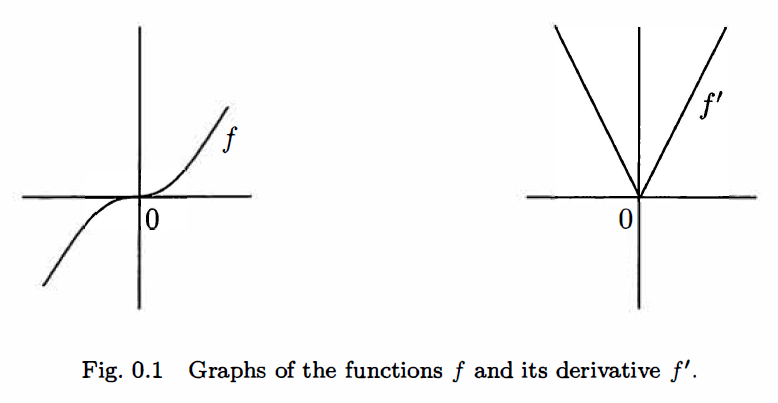
\includegraphics[width=0.6\textwidth]{./SaltChapter/preface-fig-0-1}
\end{center}
\label{fig:0.1}
\caption{함수 $f$와 도함수 $f'$의 그래프}
\end{figure}

그러면 $f$는 모든 점에서 미분가능하며 다음과 같이 쓸 수 있다.
\begin{equation}\label{eq0.1}
f'(x) = \begin{cases} 2x, & x\ge 0, \\ -2x, & x<0. \end{cases}
\end{equation}
$x\ne0$일 때는 $f'(x)$를 직접 계산하여 구할 수 있고,
$f'(0)=0$임을 다음과 같이 보일 수 있다. \\
$x\ne0$에 대하여
$$
\left| \frac{f(x) - f(0)}{x-0} - 0\right|  = \left| \frac{f(x)}{x}\right| = \frac{|x|^2}{|x|} = |x| = |x-0|
$$
이므로 주어진 $\epsilon>0\,$에 대하여 
$\delta = \epsilon (>0)$으로 잡으면
$0<|x-0|<\delta$일 때, 
$$
\left| \frac{f(x) - f(0)}{x-0} - 0\right|  = |x-0| <\delta = \epsilon
$$
을 얻는다.
하지만, $f'$은 원점 $x=0$에서 미분가능하지 않다.
증명은 연습문제 \ref{ex-0-1}를 참고하라.
요약하면, 함수 $f:\mathbb R \to \mathbb R$는 모든 실수에서 미분가능하지만 
그 도함수 $f'$은 모든 점에서 미분이 가능하지는 않다.

이와 대조적으로, 복소함수 $F:\mathbb C \to \mathbb C$가
모든 복소수에서 복소미분가능하다면, 무한번 복소미분가능함을 공부할 예정이다.
특히, 도함수 $F'$도 모든 복소수에서 복소미분가능하다.
실해석학에 익숙하다면 이는 분명 예상을 벗어난 결과이다.
우리는 복소해석학에서 이러한 놀라운 결과가 발생하는 이유에 대하여 살펴볼 예정인데,
복소미분가능하다는 것은 이러한 현상을 가능하게 하는 ``엄밀한'' 조건을 내포하고 있다.
또한, 이 엄밀함은 복소수의 곱셈의 기하학적인 특성에 따른 결과임을 보일 것이다.
\hfill $\diamondsuit$
\end{salt_example}

\begin{salt_exercise} \label{ex-0-1}
식 \eqref{eq0.1}에서 정의된 함수 $f':\mathbb R \to \mathbb R$는 $0$에서 미분 불가능함을 보여라.
\end{salt_exercise}

%=====
\section*{왜 복소해석학을 공부하는가?}

복소해석학이 단지 실해석학의 색다른 일반화로만 보일지 모르지만 사실 그렇지 않다. 
복소해석학은 수학의 모든 분야에서 필수적이다.
실제로 실해석학과 복소해석학은 뗄 수 없는 관계에 있으며,
응용 과학분야에서도 복소해석학은 중요한 역할을 하고 있음을 살펴볼 예정이다.
여기서는 복소해석학을 공부해야 하는 몇가지 이유를 간단히 나열해보자.

\begin{itemize}
\item[(1)] {\bf 편미분방정식:}  복소미분가능한 함수 $f:\mathbb C \to \mathbb C$ 의 
실수부와 허수부 $u,v: \mathbb R^2 \to \mathbb R\,$는 실함수가 되며, 
$(x,y)\in \mathbb R^2$에 대하여 $u(x,y) := \Re(f(x,y))$, $v(x,y):=\Im(f(x,y))$로 쓸 수 있다.

\begin{figure}[!h]
\begin{center}
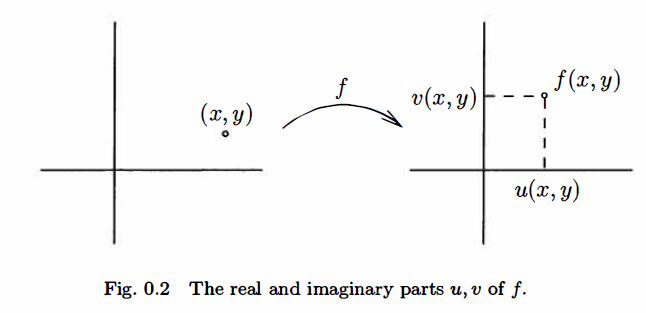
\includegraphics[width=0.5\textwidth]{./SaltChapter/preface-fig-0-2}
\end{center}
\label{fig:0.2}
\caption{복소함수 $f$의 실수부 $u$와 허수부 $v$}
\end{figure}

실수부와 허수부는 라플라스 방정식이라 불리는 중요한 편미분방정식을 만족한다:
$$
\Delta u := \frac{\partial^2 u}{\partial x^2} + \frac{\partial^2 u}{\partial y^2} = 0.
$$
마찬가지로 $\Delta v=0$도 성립한다.
라플라스 방정식은 물리학과 같은 많은 응용문제에서 유도되는 중요한 방정식이다.
예를 들면, 전자기학, 시간에 불변하는 열전도 방정식, 비압축성 유체, 브라운 운동 등에 사용된다.

\item[(2)] {\bf 실해석:} 복소해석학을 이용하면, 다음 실적분을  쉽게 계산할 수 있다.
$$
\int_{-\infty}^\infty \frac{\cos x}{1+x^2}dx, 
\quad
\int_0^\infty \cos(x^2)dx.
$$
이 문제들은 실수에서 정의된 것이나 복소해석학을 이용하여 풀 수 있다.

또한, 복소해석학을 이용하면 실해석학에서 발생하는 문제들을 명확히 할 수 있다.
예를 들어 다음 함수를 생각해보자.
$$
f(x):= \frac{1}{1-x^2}, \quad
x\in \mathbb R \setminus \{-1,1\}.
$$
그러면 $f$는 $x=\pm1$에서 정의되지 않아 특이점을 갖는다.
하지만, 구간 $(-1,1)$에서는 잘 정의된다.
등비급수
$$
1+x^2+x^4+x^6 +\cdots
$$
는  $|x^2|<1$에서, 즉, $|x|<1$에서 수렴하므로 $x\in (-1,1)$에 대하여
$$
1+x^2+x^4+x^6 +\cdots = \frac{1}{1-x^2} = f(x).
$$
$f$가 $x=1$과 $x=-1$에서 특이점을 가지므로 위의 급수표현은 $x\in(-1,1)$에 대해서만 유효함은 당연해 보인다.
이제 새로운 함수 $g$를 다음과 같이 생각해보자.
$$
g(x):= \frac1{1+x^2}, \quad x\in \mathbb R.
$$
등비급수
$$
1-x^2+x^4-x^6 +\cdots
$$
는  $|-x^2|<1$에서, 즉, $|x|<1$에서 수렴하므로 $x\in (-1,1)$에 대하여
$$
1-x^2+x^4-x^6 +\cdots = \frac{1}{1+x^2} = g(x).
$$
따라서 
$g$는 $x=1$과 $x=-1$에서 특별히 문제가 될 이유가 없음에도 불구하고
함수 $g$도 $x\in(-1,1)$에 대해서만 유효한 급수표현을 갖는다.
이 미스테리는 책의 후반부에서 해결할 예정이며 다음 복소함수를 살펴볼 필요가 있다.
$$
F(z) = \frac1{1-z^2} \quad
G(z) = \frac1{1+z^2}
$$
두 함수의 정의역을 $\mathbb R$로 한정하면 각각 $f$와 $g$를 얻는다.
특히, 복소함수 $G$는 이제 $z=\pm i$에서 특이점을 갖는다.
그림에서 $z=0$을 중심으로 급수 전개가 유효한 최대 원판은
$G$의 특이점을 포함하지 않아야 함을 알 수 있다.

\begin{figure}[!h]
\begin{center}
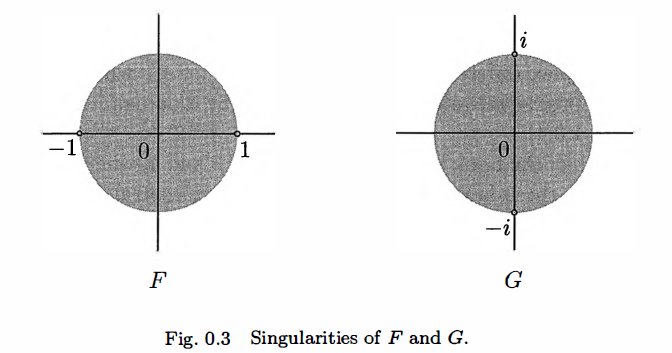
\includegraphics[width=0.6\textwidth]{./SaltChapter/preface-fig-0-3}
\end{center}
\label{fig:0.3}
\caption{복소함수 $F$와 $G$의 특이점}
\end{figure}

\item[(3)] {\bf 응용 문제:}  푸리에 변환, 라플라스 변환, z-변환과 같이 응용 문제 해결에 사용되는 많은 도구들은
복소함수 이론에 의존한다. 이  도구들은 여러 응용 분야에서 나타나는 미분방정식의 해결에 유용하다.
복소해석학은 수리물리와 공학분야의 응용에 중요한데, 예를 들면, 제어이론, 신호처리 등이 있다.

\item[(4)] {\bf 해석 정수론:}
자연수와 관련된 많은 문제가 복소해석학을 이용하여 해결된다는 것은 아마도 놀라울 것이다.
예를 들면, 소수정리는 큰 자연수 $n$에 대하여 $n$보다 작은 소수의 개수 $\pi(n)$을 
점근적으로 판정하는 방법을 알려준다.

\begin{salt_theorem}{\bf (소수정리)}
$$
\lim_{n\to\infty} \frac{\pi(n)}{n/(\log n)} = 1.
$$
\end{salt_theorem}

소수정리는 리만 제타함수라는 복소미분가능 함수의 성질을 이용하여 증명할 수 있음이 밝혀졌다.
리만 제타함수와 관련된 해석 정수론의 유명한 미해결 문제로 리만가설이 있다.
리만 제타함수의 모든 비자명해는 복소평면에서 직선 $\Re(s)=\frac12$ 위에 존재한다는 것이다.
우리는 리만 제타함수를 연습문제 \ref{ex-4-5}에서 만날 것이다.
\end{itemize}


\section*{복소해석학에서는 무엇을 배우는가?'}

이 과정의 중심이 되는 주제는 다음과 같다.

%\begin{center}
\fbox{\begin{minipage}{\dimexpr\textwidth-15\fboxsep-2\fboxrule\relax}
\begin{center}
복소영역에 정의된 복소해석함수들
\end{center}
\end{minipage}}
%\end{center}

즉, 복소영역 $D$에 정의된 복소미분가능 함수 $f \colon D\to \mathbb C$가 대상이다.
``복소영역'' $D$에 대한 정확한 의미는 1.3.4 절에서 다룬다.

책의 중심인 2, 3, 4장에서는 
핵심 주제인 복소해석(holomorphic) 함수에 빛을 비춰줄 다음 3가지를 다룬다.
\begin{enumerate}
\item[(1)] 코시-리만 방정식
\item[(2)] 코시 적분 정리
\item[(3)] 테일러 급수
\end{enumerate}

\begin{figure}[!h]
\begin{center}
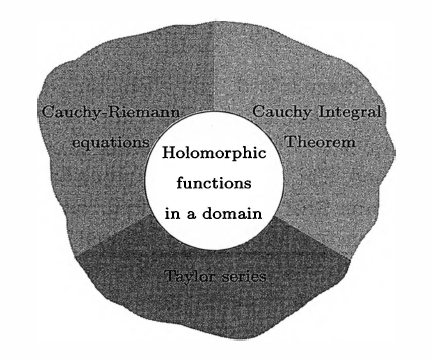
\includegraphics[width=0.5\textwidth]{./SaltChapter/preface-fig-0-4}
\end{center}
\end{figure}

%다음 정리는 책에서 공부할 핵심적인 내용을 요약한 것이다.
다음은 이 책의 핵심정리이다.

\begin{salt_theorem}
경로연결된 열린집합 $D$에 정의된 함수
$f:D\to \mathbb C$에 대하여 다음은 동치이다.
\begin{itemize}
\item[(1)] $D$의 모든 점 $z$에서 $f'(z)$가 존재한다.
\item[(2)] $D$의 모든 점 $z$에서 모든 차수 ($n\ge0$)의 미분  $f^{(n)}(z)$가 존재한다.
\item[(3)] 실수부와 허수부 $u:=\Re(f)$, $v:=\Im(f)$는 연속미분가능하며 
$$
\frac{\partial u}{\partial x} = \frac{\partial v}{\partial y},
\quad
\frac{\partial u}{\partial y} = - \frac{\partial v}{\partial x}
$$
을 만족한다.
\item[(4)] $D$의 단순연결 부분영역 $S$에 대하여 
복소해석함수 $ F: S\to \mathbb C$가 존재하여
$S$의 모든 점 $z$에서 $F'(z)= f(z)$를 만족한다.
\item[(5)] $ f$ 가 $D$에서 연속이고, 
$D$의 모든 단순연결 부분영역에서
임의의 조각마다 매끄러운 닫힌곡선 $\gamma$에 대하여 다음이 조건이 성립한다.
$$
\int_\gamma f(z)dz = 0.
$$
\item[(6)] $\{ z\in \mathbb C\,:\, |z-z_0| \le r \} \subset D$이면
$|z-z_0|<r$을 만족하는 임의의 $z$에 대하여
$$
f(z) = \sum_{n=0}^\infty c_n(z-z_0)^n
$$
을 만족하는 복소수열 $(c_n)_{n\ge0}$이 유일하게 존재한다.
부가적으로 계수 $c_n$는 다음식으로 구할 수 있다.
$$
c_n = \dfrac1{2\pi i} \dint_{|\zeta-z_0|=r} \frac{f(\zeta)}{(\zeta-z_0)^{n+1}}d\zeta = \dfrac{f^{(n)}(z_0)}{n!}.
$$
\end{itemize}
\end{salt_theorem}

\section*{복소해석학은 복잡한 해석학이 아니다!}


실제로 아주 복잡한 것이 아니며,  지나치게 해석적인 것도 아니다.
복소해석학은 실해석학보나 오히려 유연하다.
복소미분의 핵심 개념 몇가지를 정립하고 나면 
입실론-델타($\epsilon$-$\delta$)를 포함한 정교한 기법들은 적게 사용된다.
앞의 핵심정리를 보면 실해석학과 근본적으로 다른 결과가 도출됨을 예상할 수 있다.
예를 들어 실함수가 열린구간 $(a,b)$에 정의된 미분가능할 때 그 도함수는 연속함수가 아닐 수 있다.
반면 복소평면 $\mathbb C$의 열린집합에 정의된 복소미분가능함수는 
무한번 미분가능하다!
그 이유는 복소곱셈이 특별한 기하학적 의미를 갖기 때문인데
복소미분가능함수는 국소적인 성질로 전체가 규정되며 
함수값을 임의로 매핑하는 것을 허용하지 않는다.
이렇게 제어되는 성질이 복소함수를 한정적으로 만드는데
2.3절에서 이를 자세히 살펴볼 예정이다.
그럼에도 불구하고 자명하지 않으며 충분히 흥미로운 주제이다!

\section*{대상 독자}

복소함수론은 미적분학과 다변수 미적분학을 학습한 학생을 대상으로 하는 기초 과정이다.
책의 제목에서 짐작할 수 있듯이
가장 최소한의 선수지식으로 학습할 수 있는 복소함수의 핵심적인 내용을 담고 있다.
이 책은 저자가 수학과 및 경제학과 3학년 학생을 대상으로 강의했던 강의록을 
바탕으로  만들어졌다.


\section*{감사의 글}

 많은 유용한 의견을 보내준 
Raymond Mortini, Adam Ostazewski, Rudolf Rupp에게 감사드린다.
참고문헌 목록에 있는 기존 학습자료에 의존하였으며
이는 연습문제의 경우도 마찬가지다.
몇가지 경우는 각 장의 끝에 ``참고'' 절을 넣고 상세한 참고문헌을 제시했지만
참고 절을 넣지 않은 경우에도 이 책만의 독창성을 주장하는 것은 아니다.

\begin{flushright}
2013년, 런던과 룬트에서

Sara Maad Sasane과 Amol Sasane
\end{flushright}



%===[salt] 1장
% !TEX root = ../notes_template.tex

\chapter{복소수와 기하학적 의미}


이 장에서는 복소해석학을 펼칠 무대를 만들기 위해
다음 3가지 중심 주제를 다룬다.

\begin{itemize}
\item[(1)] 복소수의 집합과 연산을 정의하고 실수체의 확장으로서 복소수체 $\mathbb C$를 만든다.
\item[(2)] $\mathbb C$의 원소는 평면 $\mathbb R^2$위의 점으로 표시할 수 있으며, 복소수체 $\mathbb C$의 연산에 대하여
기하학적 의미를 부여할 수 있다. 복소수체와 평면위의 점의 대응 관계로부터
$\mathbb C$에 평면의 유클리드 위상을 가져올 수 있다.
\item[(3)] 끝으로 복소해석학의 기초함수인 지수함수를 공부한다.
또한, 지수함수와 관련된 기본함수인 삼각함수와 로그함수도 살펴본다. 
\end{itemize}

\section{복소수체}

{\bf 복소수}는 실수의 순서쌍으로 정의한다. 예를 들면,
$$
(1,0), \ (0,1), \ (0,0), \ \left(-\dfrac34, \sqrt{2} \right)
$$
는 모두 복소수로 간주할 수 있다.
복소수 전체의 집합 $\mathbb R \times \mathbb R$을 $\mathbb C$라 표기한다. 즉,
$$
\mathbb C = \left\{ z = (x,y) \,:\, x\in \mathbb R, \text{ 이고 } y\in \mathbb R \right\}.
$$

복소수 $z=(x,y)\in \mathbb C$ ($x,y \in \mathbb R$)에 대하여
실수 $x$는 $z$의 실수부, $y$는 $z$의 허수부라고 한다.

집합 $\mathbb C$의
복소수 $(x_1, y_1)$, $(x_2, y_2)$에 대하여
덧셈 ``$+$''과 곱셈 ``$\cdot$''을 다음과 같이 정의한다.
\begin{gather*}
(x_1, y_1) + (x_2, y_2) = (x_1+x_2, y_1+y_2), \\
(x_1, y_1) \cdot (x_2, y_2) = (x_1x_2 - y_1y_2, x_1y_2 + x_2y_1).
\end{gather*}
이 연산에 따라 $\mathbb C$는 체(field)가 된다. 즉,
\begin{itemize}
\item[(F1)]  $(\mathbb C, +)$는 가환군(Abelian group)이다.
\item[(F2)] $(\mathbb C\setminus \{0\}, \cdot)$는 가환군이다.
\item[(F3)] $a,b,c\in\mathbb C$에 대하여 분배법칙이 성립한다:  $(a+b)\cdot c = a\cdot c + b\cdot c$.
\end{itemize}

(F1)에서 가환군이란
연산 $+$에 대하여 결합법칙, 교환법칙이 성립하며,
모든 $(x,y)$에 대하여
$$
(x,y) + (0,0) = (x,y) = (0,0) + (x,y)
$$
를 만족하는 
항등원 $(0,0)$과 
$$
(x,y) + (-x,-y) = (0,0) = (-x,-y) + (x,y)
$$
를 만족하는 덧셈의 역원 $(-x, -y)$이  존재한다는 뜻이다.

유사하게, (F2)에서 곱셈의 항등원 $(1,0)$이 존재하고, 복소수 $(x,y) \in \mathbb C \setminus\{0,0\}$의
곱셈의 역원은 다음과 같다.
\begin{equation} \label{eq:1.1}
\left( \dfrac{x}{x^2+y^2}, \dfrac{-y}{x^2+y^2} \right).
\end{equation}

\begin{salt_exercise}
식 \eqref{eq:1.1}\이 복소수 $(x,y) \in \mathbb C \setminus\{0,0\}$의 곱셈의 역원이 됨을 직접 확인하라.
\end{salt_exercise}


\begin{salt_prop}
$(\mathbb C, +, \cdot)$는 체(field)이다.
\end{salt_prop}

실수  $\mathbb R$은 복소수 $\mathbb C$에 ``포함된다''.
실제로, 복소수 $\mathbb C$안에 $\mathbb R$을 넣어
실수 $\mathbb R$을 $\mathbb C$의 부분체(subfield)로 볼 수 있다.
$$
x \mapsto (x,0)
$$
을 이용하여 실수 $x$를 복소수 $(x,0)$로 보내는 대응 규칙은
단사인 체의 준동형사상(field homomorphism)이다.
즉, 덧셈과 곱셈이 보존되며 서로 다른 실수는 다른 복소수에 대응시키는 사상이다.

\begin{center}
\begin{tabular}{|ccc|} \hline
$\mathbb R$ & & $\mathbb C$ \\ \hline \hline
$x$ & $\mapsto$ & $(x,0)$ \\ 
$x_1+x_2$ & $\mapsto$ & $(x_1+x_2,0) = (x_1,0) + (x_2,0)$ \\ 
$x_1\cdot x_2$ & $\mapsto$ & $(x_1\cdot x_2,0) = (x_1,0) \cdot (x_2,0)$ \\ 
$1$ & $\mapsto$ & $(1,0)$ \\
$0$ & $\mapsto$ & $(0,0)$ \\
\hline
\end{tabular}
\end{center}

따라서 이 사상을 이용한 동일화에 따라 모든 실수는 복소수로 볼 수 있다.
예를 들어 실수 $\sqrt{2}$는 복소수 $(\sqrt{2},0)$로 볼 수 있다.
이런 생각에 익숙하지 않을 수도 있겠으나 우리는 이미 초등학교 과정에서
비슷한 동일화를 경험한 적이 있다. 정수를 유리수의 일부로 동질화하는
다음 예를 보자.
$$
\mathbb Z  \ni 3 = \frac31 \in \mathbb Q
$$
이를 이해하려고 밤잠을 설친 적은 없지 않은가!

실수 해 $x\in\mathbb R$를 갖지 않는 방정식
$$
x^2+1=0
$$
을 복소수 밤위에서 다루면 해를 구할 수 있다.
$$
(0,1)\cdot (0,1) + (1,0) = (-1,0) + (1,0) = (0,0).
$$
$(0,1)$을 나타내는 특별한 기호로 $i$를 도입하면 이 방정식을 다음과 같이 쓸 수 있다.
$$
i^2+1=0,
$$
여기서 실수 $1$과 $0$은 각각 복소수 $(1,0)$과 $(0,0)$에 대응된다.

이제부터 실수  $x,y$로 만든 복소수 $(x,y)$를 $x+yi$로 쓰자.
$$
(x,y) = \underbrace{(x,0)}_{\equiv x} +  \underbrace{(y,0)}_{\equiv y}
\cdot  \underbrace{(0,1)}_{\equiv i} = x+yi.
$$
복소수 곱셈은 교환법식이 성립하고, 특히 $yi = iy$이므로,
$x+yi = x+iy$이다.

\begin{salt_exercise} %1.2
$\theta \in \left(-\dfrac{\pi}2, \dfrac\pi2 \right)$에 대하여
$\dfrac{1+i\tan\theta}{1-i\tan\theta}$를 $x+yi$ 꼴로 표시하면?
\end{salt_exercise}

{\bf 복소수 발견의 역사: }
대중적인 믿음과는 달리 역사적으로 수학자들이 복소수를 진지하게 받아들이게 된 것은 
2차 방정식이 아니라 3차 방정식을 풀 필요가 있었기 때문이다. 요지는 다음과 같다.
16세기 경 포물선 $y=x^2$과 직선 $y=-bx-c$의 교점을 구하는  방법으로 
 방정식
$$
ax^2 + bx + c = 0
$$
을 풀려는 시도가 있었다. 
이러한 기하학적 해석에 근거하여,
포물선  $y=x^2$ 이 직선 $y=-1$과 만나지 않으므로
실계수 2차방정식 $x^2+1=0$이 실수해를 갖지 않음을 쉽게 알 수 있었다.
%%%%%%
그림 \ref{fig-1-1}의 왼쪽 그래프를 참고하라.

\begin{figure}[!h]
\begin{center}
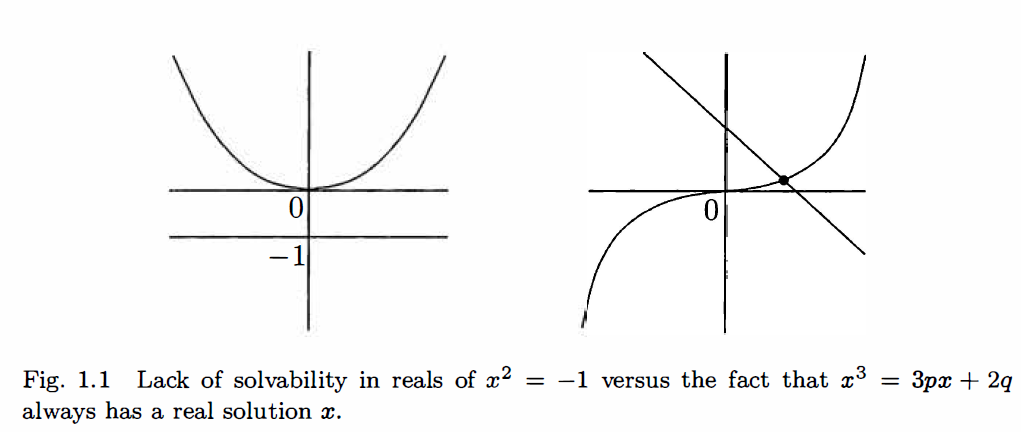
\includegraphics[width=0.6\textwidth]{./SaltChapter/fig-1-1}
\end{center}
\caption{실근이 존재하지 않는 방정식 $x^2=-1$과 항상 실근을 갖는 $x^3=3px+2q$}
\label{fig-1-1}
\end{figure}

Cardano (1501-1576)는 3차방정식 $x^3=3px+2q$의 실근을 구하는 다음 공식을 만들었다.
$$
x = \sqrt[3]{q+ \sqrt{q^2-p^3}} + \sqrt[3]{q- \sqrt{q^2-p^3}}
$$
예를 들어, $p=2$, $q=3$일 때 방정식 $x^3=6x+6$은 $x=\sqrt[3]{4}+\sqrt[3]{2}$를 해로 가진다.
한편, 중간값 정리에 의해 3차함수 $y=x^3$은  항상 $y=3px+2q$와 만난다.
그림 \ref{fig-1-1}의 오른쪽 그래프를 참고하라.
하지만 $p=5$, $q=2$로 방정식 $x^3=15 x+4$을 만들면 $q^2-p^3= -121<0$이 되어
실수만으로는 Cardano의 공식을 적용하지 못한다.
그럼에도 불구하고 우리는 $x=4$가 실근이 됨을 확인할 수 있다.
$$
4^3 = 64 = 60 + 4 = 15\cdot 4 + 4.
$$
Cardano 공식이 나온지 30년 후, Bombelli가 복소수 연산을 도입하면
Cardano 공식으로 원하는 실근을 도출할 수 있음을 제안하였다.
다음 등식이 성립할 수 있을까?
$$
x = \sqrt[3]{2+11i} + \sqrt[3]{2-11i} \stackrel{?}{=} 4.
$$
$(2+i)^3 = 2+11i$이고 $(2-i)^3 = 1-11i$임을 이용하면
세제곱근 값으로부터 위 등식이 성립함을 알 수 있다.
따라서 Bombelli의 결과로부터 실수 문제에도 복소수 연산이 연결될 수 있음이 입증되었다.
그때부터 복소수가 수학의 주류에 들어가게 되었다.

\begin{salt_exercise} \label{ex-1-3}
양의 부분집합 $P\subset \mathbb F$가 있어 다음을 만족하면
체 $\mathbb F$는 순서(ordered)를 갖는다고 한다.
\begin{itemize}
\item[(P1)] 모든 $x,y\in P$에 대하여, $x+y\in P$.
\item[(P2)] 모든 $x,y\in P$에 대하여, $x\cdot y \in P$
\item[(P3)] 모든 $x\in P$에 대하여, 다음 3가지 중  정확히 한가지만 참이다.
$$
1^{\circ} \ x=0. \quad 2^{\circ} \ x\in P. \quad 3^{\circ} \ -x\in P.
$$
\end{itemize}
예를 들면, $P:=(0,\infty)$를 양의 부분집합이라 하면
실수체 $\mathbb R$은 순서를 갖는다.
( 순서를 갖는 체 $\mathbb F$에서 두 원소 $x,y\in \mathbb F$의 관계 $>_P$를
$y>_P x$는 $y-x \in P$로 정의하여 대소관계를 정할 수 있다.)
복소수 $\mathbb C$는 순서를 가질 수 없음을 보여라. \\[1ex]
힌트: $x:=i$에 대하여 $x\cdot x$를 살펴보라.
\end{salt_exercise}

\section{복소수의 기하학적 표현}

$\mathbb C = \mathbb R^2$이므로, 
그림 \ref{fig-1-2}와 같이 복소수를 평면위의 점에 대응시킬 수 있다.

\begin{figure}[!h]
\begin{center}
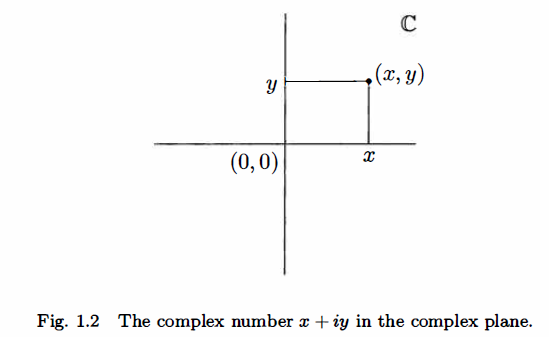
\includegraphics[width=0.5\textwidth]{./SaltChapter/fig-1-2}
\end{center}
\caption{복소평면에 표시한 복소수 $x+iy$}
\label{fig-1-2}
\end{figure}

복소평면은 Argrand\footnote{ 
Jean-Robert Argand (1768-1822)의 이름에서 따온 것이다.
Caspar Wessel (1745-1818)이 더 먼저 사용하긴 했으나.}
평면이라고도 불린다.

\begin{salt_exercise} \label{ex-1-4}
다음 복소수를 복소평면 위의 점으로 표시하라.
$$
0, \quad 1 , \quad -\frac32, \quad i, \quad -\sqrt{2}i,
\quad \cos \frac\pi3 + i\sin\frac\pi3.
$$
\end{salt_exercise}

따라서 복소수 $\mathbb C$는 {\bf 집합}으로서 평면 $\mathbb R^2$로 간주할 수 있다.
$\mathbb C$에 정의된 체의 연산이 평면에서 기하학적 의미를 가질까?
우리는 앞으로 실제로 의미가 있음을 살펴볼 것이다.
$\mathbb C$의 덧셈은 평면벡터의 덧셈이고
곱셈은 조금 더 특별한 의미를 갖는다.

{\bf 복소수 덧셈의 기하학적 의미: }
복소수를 평면 위의 점으로 간주하고 복소수의 덧셈을 $\mathbb R^2$의 벡터 합으로 
정의하는 것이 자연스럽다. 
벡터 합은 두 벡터를 결합하는 일반적인 방식으로 정의한다.
즉, $(0,0)$과 두 복소수를 잇는 선분으로 이루어진 평생사변형을 완성시킬 때
$(0,0)$과 대각선의 반대에 있는 점을 두 복소수의 합이 된다.
그림 \ref{fig-1-3}\을 참고하라.

\begin{figure}[!h]
\begin{center}
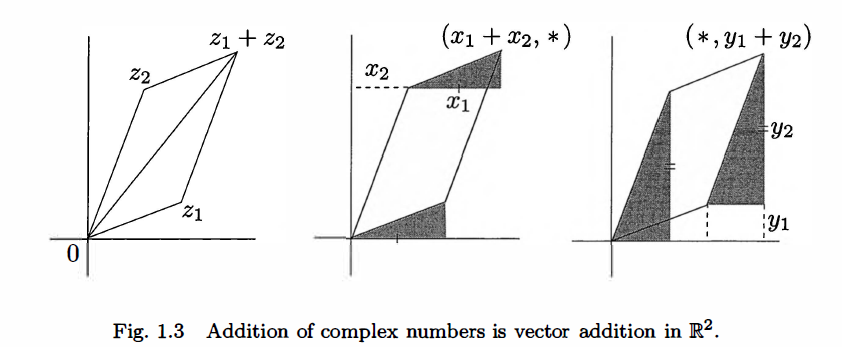
\includegraphics[width=0.8\textwidth]{./SaltChapter/fig-1-3}
\end{center}
\caption{복소수 덧셈은 $\mathbb R^2$의 벡터 합이다.}
\label{fig-1-3}
\end{figure}

{\bf  복소수 곱셈의 기하학적 의미: }
이제 복소수 곱셈이 가진 특별한 기하학적 의미를 살펴보자.
이를 위해 편의상 극좌표를 사용한다.
$(x,y)\in\mathbb R^2$이 극좌표 $r\ge 0$와 $\theta\in(-\pi,\pi]$로 표현된다고 하자.
이는 원점에서 $(x,y)$까지의 거리를 $r(\ge0)$이고,
$(0,0)$에서 $(x,y)$를 잇는 반직선이 $x$-축의 양의 방향과 이루는 각이 $\theta$가 된다는 뜻이다.
($(x,y)$가 원점 $(0,0)$인 경우, $\theta=0$으로 정한다.)

\begin{figure}[!h]
\begin{center}
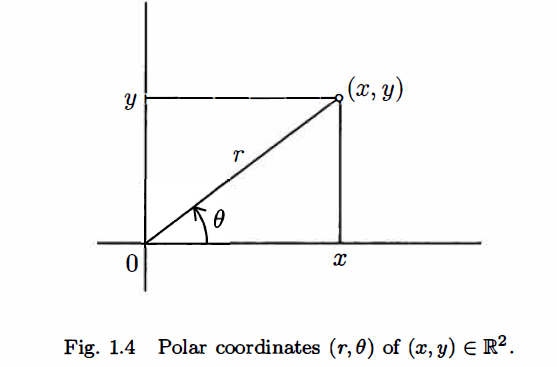
\includegraphics[width=0.5\textwidth]{./SaltChapter/fig-1-4}
\end{center}
\caption{복소수 $(x,y)\in\mathbb R^2$의 극좌표 표현 $(r, \theta)$}
\label{fig-1-4}
\end{figure}

그림 \ref{fig-1-4}의 직각삼각형으로부터 다음 관계를 얻는다.
\begin{gather*}
x = r \cos\theta, \\
y = r \sin \theta.
\end{gather*}
이로부터 복소수를 극좌표 $(r,\theta)$로 표현할 수 있다.
$$
x + yi = r\cos\theta +(r\sin \theta)i
= r(\cos\theta + i\sin \theta).
$$
이제 복소수 곱셈의 기하학적으로 해석하자.
두 복소수를 모두 극좌표로 쓰면
\begin{gather*}
z_1 = r_1 (\cos\theta_1 + i\sin\theta_1), \\
z_2 = r_2 (\cos\theta_2 + i\sin\theta_2),
\end{gather*}
삼각함수의 덧셈정리로부터 다음을 얻는다.
\begin{align*}
z_1\cdot z_2 &= r_1(\cos\theta_1+i\sin\theta_1) \cdot r_2(\cos\theta_2+i\sin\theta_2) \\
&= r_1r_2 (\cos\theta_1\cos\theta_2 - \sin\theta_1\sin\theta_2 +
i(\cos\theta_1\sin\theta_2 + \cos\theta_2\sin\theta_1)) \\
&= r_1r_2(\cos(\theta_1 +\theta_2) + i \sin(\theta_1 +\theta_2)).
\end{align*}
따라서 $z_1\cdot z_2$는 극좌표로 $(r_1r_2, \theta_1+\theta_2)$이다.
다시 말하면, 
$z_1\cdot z_2$의 편각은
$z_1$과 $z_2$가 각각 실수축의 양의 방향과 이루는 각을 더하여 얻을 수 있고,
원점에서의 거리는 각각의 거리를 곱하여 얻는다.
그림 \ref{fig-1-5}\를 참고하라.

\begin{figure}[!h]
\begin{center}
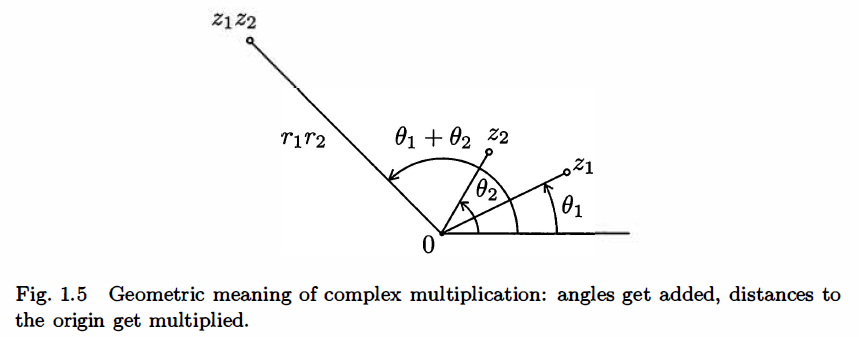
\includegraphics[width=0.5\textwidth]{./SaltChapter/fig-1-5}
\end{center}
\caption{복소수 곱셈의 기하학적 의미: 각은 더하고, 원점에서의 거리는 곱한다.}
\label{fig-1-5}
\end{figure}

특별한 경우로 원점에서의 거리가 $1$인 복소수
$\cos\alpha + i \sin\alpha$를 곱하는 경우를 생각해보자.
그러면 위의 식으로부터 $z\in\mathbb C$와의 곱
$z\cdot(\cos\alpha + i\sin\alpha)$는 
원점과 $z$를 연결하는 직선을 반시계방향으로 $\alpha$만큼 회전시켜 얻을 수 있다.
특히, $z$에 
$$
i = 0 + i\cdot 1 = \cos\frac\pi2 + i \sin\frac\pi2
$$
를 곱하면 반시계방향으로 $90^{\circ}$ 회전한 결과를 얻는다.

\begin{figure}[!h]
\begin{center}
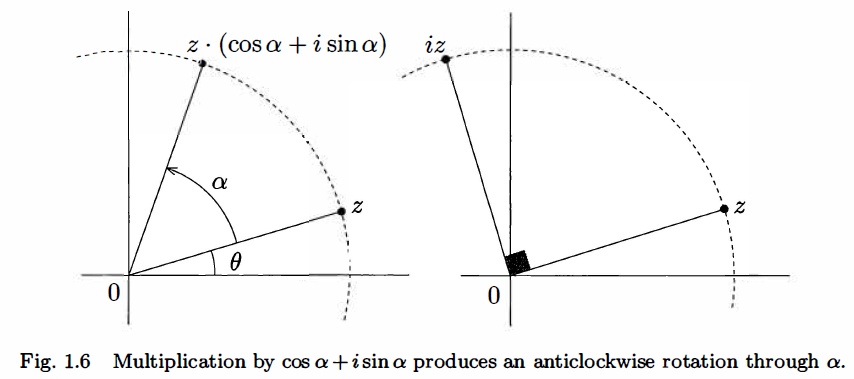
\includegraphics[width=0.8\textwidth]{./SaltChapter/fig-1-6}
\end{center}
\caption{$\cos\alpha + i \sin\alpha$를 곱하면 반시계방향으로 $\alpha$만큼 회전한 결과를 얻는다.}
\label{fig-1-6}
\end{figure}

{\bf 드 므와브르(De Moivre) 정리와 $n$차 제곱근 :}
모든 자연수 $n\in\mathbb N$에 대하여
$$
(\cos\theta + i\sin\theta)^n = \cos(n\theta) + i\sin(n\theta)
$$
가 성립하며 이를 드 므와브르 정리라 한다.

\begin{salt_exercise} \label{ex-1-5}
드 므와브르의 정리를 이용하여
삼각함수의 3배각 공식 $\cos (3\theta) = 4(\cos\theta)^3 - 3\cos\theta$을 증명하라.
\end{salt_exercise}

\begin{salt_exercise} \label{ex-1-6}
$(1+i)^{10}$을 직접 전개하지 않고 $x+iy$ ($x,y$는 실수)의 꼴로 써라?
삼각함수의 3배각 공식 $\cos (3\theta) = 4(\cos\theta)^3 - 3\cos\theta$을 증명하라.
\end{salt_exercise}

\begin{salt_exercise} \label{ex-1-7}
$(2+i)(3+i)$를 이용하여
$\dfrac\pi4 = \tan^{-1}\dfrac12 + \tan^{-1}\dfrac13$을 증명하다.
\end{salt_exercise}

\begin{salt_exercise} \label{ex-1-8}
가우스 정수(Gaussian integer)는 
$m, n$이 정수일 때, $m+in$꼴의 복소수로
복소평면 위의 정수 격자점을 이룬다.
모든 꼭지점이 가우스 정수가 되도록 정삼각형을 그리는 것을 불가능함을 증명하라. \\[1ex]
힌트: 한변의 회전으로 다른 변을 만들 수 있고, $\sqrt{3}\not\in \mathbb Q$임을 이용하라.
\end{salt_exercise}

드 므와브르 공식을 이용하면
복소수  $z$의 $n$ 제곱근
즉, $w^n=z$를 만족하는 복소수 $w$를 쉽게 구할 수 있다.
우선 적당한 $r\ge0$과 $\theta\in[0,2\pi)$에 대하여 $z=r(\cos\theta + i \sin\theta)$로 쓰자.
$w= \rho(\cos\alpha + i\sin\alpha)$가 $w^n=z$를 만족한다면,
$$
w^n = \rho^n\left( \cos(n\alpha) + i\sin(n\alpha)\right) = r(\cos\theta + i\sin\theta)= z.
$$
양변은 원점에서의 거리가 같으므로 $\rho^n=r$을 얻는다.
$\rho$와 $r$이 음수가 아니므로 $\rho = \sqrt[n]{r}$이다.
한편 $w^n$이 실수축의 양의 방향과 이루는 각 $n\alpha$는 
집합 $ \{ \ldots, \theta - 4\pi, \theta - 2\pi, \theta, \theta+2\pi, \theta+4\pi, \ldots\} $에 속한다.
$0$이 아닌 $z$가 실수축의 양의 방향과 이루는 각은 $2\pi$의 정수배 차이를 무시하면 유일하게 결정되므로
$\theta$ 대신 $\theta + 2\pi k$ ($k$는 정수)로도 쓴다. 그림 \ref{fig-1-7}\을 참고하라.

\begin{figure}[!h]
\begin{center}
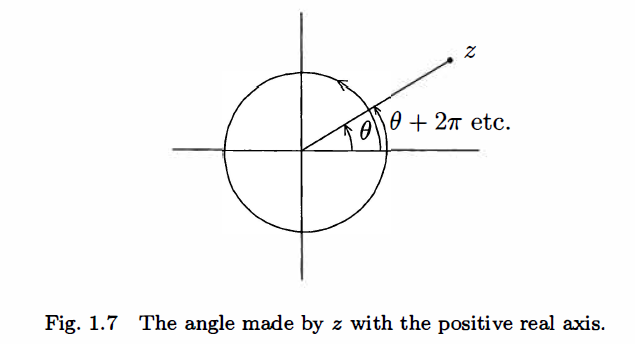
\includegraphics[width=0.7\textwidth]{./SaltChapter/fig-1-7}
\end{center}
\caption{복소수 $z$가 실수축의 양의 방향과 이루는 각}
\label{fig-1-7}
\end{figure}

이제 $\alpha \in \left\{ \dfrac{\theta}{n}+ \dfrac{2\pi}{n}k \,:\, k\in\mathbb Z \right\}$로부터
서로 다른 $w$가 되는 $\alpha$만 쓰면 다음과 같다.
$$
\alpha \in \left\{
\dfrac\theta n,  \dfrac\theta n+ \dfrac{2\pi}n, \dfrac\theta n + 2\cdot \dfrac{2\pi}n, \ldots,
\dfrac\theta n+ (n-1)\cdot \dfrac{2\pi}n
\right\}.
$$
특히, $z=1$일 때, $1$의 $n$제곱근은 원에 내접하는 정$n$각형의 꼭지점이다.
그림 \ref{fig-1-8}을 보라.
\begin{figure}[!h]
\begin{center}
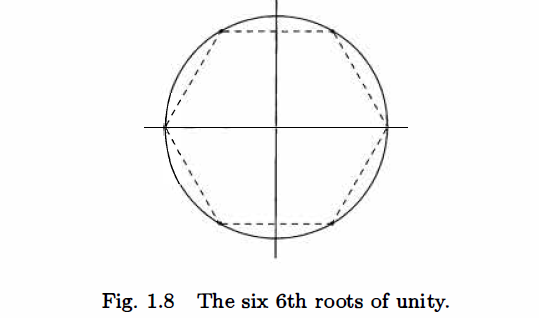
\includegraphics[width=0.7\textwidth]{./SaltChapter/fig-1-8}
\end{center}
\caption{$1$의 $6$ 제곱근 $6$개}
\label{fig-1-8}
\end{figure}

\begin{salt_exercise} \label{ex-1-9}
$w^4=-1$을 만족하는 모든 복소수 $w$를 찾아
복소평면에 표시하라.
\end{salt_exercise}

\begin{salt_exercise} \label{ex-1-10}
$z^6-z^3-2=0$을 만족하는 모든 복소수 $z$를 구하라.
\end{salt_exercise}

\begin{salt_exercise} \label{ex-1-11}
$a^2+b^2+c^2= ab+bc+ca$를 만족하는 실수 $a,b,c$는 모두 같다.
실제로 양변에 $2$를 곱하고 정리하면
$(a-b)^2+(b-c)^2+(c-a)^2=0$을 얻고, 
각 항은 음수가 아니므로 모두 $0$이 될 수밖에 없다.
한편, $a^2+b^2+c^2= ab+bc+ca$를 만족하는 복소수 $a,b,c$는
복소평면위의 정삼각형의 꼭지점이 됨을 보여라.
실수의 경우와 결과를 비교하라. \\[1ex]
힌트: 실수가 아닌 $1$의 세제곱근 $\omega$에 대하여
$((b-a)\omega + (b-c))\cdot((b-a)\omega^2 + (b-c))$를 계산하라.
\end{salt_exercise}

\begin{salt_exercise} \label{ex-1-12}
이항정리에서
$a,b$가 실수이고, $n\in\mathbb N$이면,
$$
(a+b)^n = \sum_{k=0}^n {n \choose k}a^kb^{n-k},
\quad
\text{여기서 }
{n \choose k} := \frac{n!}{k!(n-k)!}, \
k=0,1,2,\ldots, n,
$$
는 이항계수라 한다.
대수적 연산을 생각하면 이 등식은 $a,b$가 복소수인 경우에도 성립한다.
$$
{3n \choose 0} + {3n \choose 3} + {3n \choose 6} + \cdots
+ {3n \choose 3n} = \dfrac{2^{3n} + 2\cdot(-1)^n}3
$$
이 성립함을 보여라. \\[1ex]
힌트: $\omega$가 실수가 아닌 $1$의 세제곱근일 때
$(1+1)^{3n} + (1+\omega)^{3n} + (1+\omega^2)^{3n}$을 계산하라.
\end{salt_exercise}

\begin{salt_exercise} \label{ex-1-13}
복소수의 기하학적 성질을 이용하여 
사각형의 대변에 외접하는 정사각형 중심을 잇는 선분은
서로를 수직이등분함을 보여라.
\end{salt_exercise}

{\bf 절대값과 켤레복소수: }
복소수 $z=x+iy$ ($x,y\in\mathbb R$)의 절대값 $|z|$는
$$
|z| = \sqrt{x^2+y^2}
$$
로 정의한다.
피타고라스 정리에 따라 이는 $z$와 원점 사이의 거리를 나타낸다.
그림 \ref{fig-1-9}의 왼쪽을 참고하라.
$z_1, z_2\in \mathbb C$를 극좌표로 쓰거나, 직접 계산하여 확인하면
$|z_1z_2| = |z_1|\cdot |z_2|$임을 쉽게 확인할 수 있다.

\begin{figure}[!h]
\begin{center}
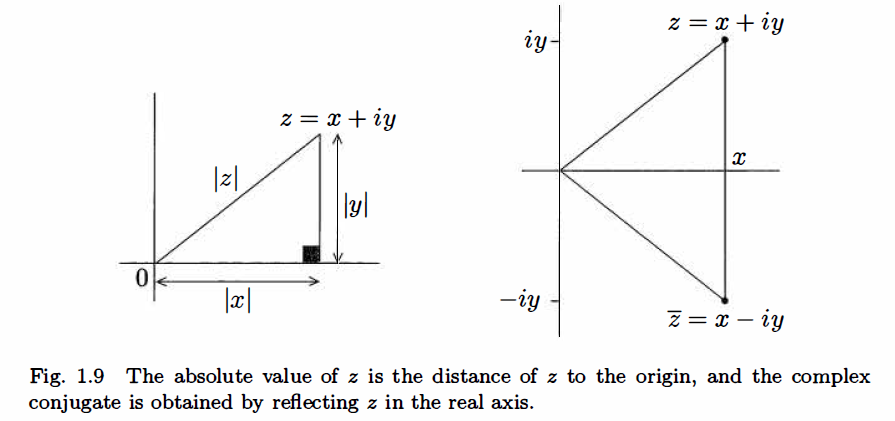
\includegraphics[width=0.7\textwidth]{./SaltChapter/fig-1-9}
\end{center}
\caption{복소수의 절대값은 원점에서의 거리이고, 켤레복소수는 실수축에 대칭인 복소수이다.}
\label{fig-1-9}
\end{figure}

\begin{salt_exercise} \label{ex-1-14}
직표좌표로 $z_1, z_2$를 써서 $|z_1z_2| = |z_1|\cdot |z_2|$임을 확인하라.
\end{salt_exercise}

복소수 $z=x+iy$ ($x,y\in\mathbb R$)의 켤레복소수 $\bar z$는
$$
\bar z = x - iy
$$
로 정의한다.
복소평면에서 $\bar z$는 $z$를 실수축으로 대칭시켜 얻는다.
그림 \ref{fig-1-9}의 오른쪽을 참고하라.
기하학적 표현으로부터 복소수 $z_1, z_2\in\mathbb C$에 대하여
다음이 성립함을 확인할 수 있다.
$$
\overline{z_1+z_2} = \overline{z_1} + \overline{z_2},
\quad
\overline{z_1\cdot z_2} = \overline{z_1} \cdot \overline{z_2}.
$$

다음 성질도 쉽게 얻을 수 있다.
$$
\bar{\bar z} = z, \quad z\bar z  = |z|^2 \quad
\Re(z) = \frac{z+\bar z}2, \quad \Im(z) = \frac{z-\bar z}{2i}.
$$

\begin{salt_exercise} \label{ex-1-15}
위의 등식 4개를 증명하라.
\end{salt_exercise}

\begin{salt_exercise} \label{ex-1-16}
모든 복소수 $z\in\mathbb C$에 대하여
$|z|=|\bar z|$, $|\Re(z)|\le |z|$, $|\Im(z)| \le z$임을 증명하고
각각에 대하여 기하학적으로 설명하라.
\end{salt_exercise}

\begin{salt_exercise} \label{ex-1-17}
$|a|<1$과 $|z|\le 1$을 만족하는 $a,z\in\mathbb C$에 대하여
$\left| \dfrac{z-a}{1-\bar a z}\right| \le 1$을 보여라.
\end{salt_exercise}

\begin{salt_exercise} \label{ex-1-18}
계수가 $c_0, c_1, \ldots, c_d\in\mathbb R$이고 $c_d\ne0$인 다항식
$p(z) = c_0+c_1z+\cdots + c_dz^d$을 생각하자.
$w\in\mathbb C$가 $p(w)=0$을 만족하면 $p(\bar w)=0$도 성립함을 보여라.
\end{salt_exercise}

\begin{salt_exercise} \label{ex-1-19}
복소수 $0, a, b \in\mathbb C$가 만드는 삼각형의 면적은
$\left| \dfrac{\Im(a\bar b)}2\right|$임을 보여라.
\end{salt_exercise}

\begin{salt_exercise} \label{ex-1-20}
임의의 복소수 $z_1,z_2, z_3$에 대하여
$i\det \begin{pmatrix}
1 & z_1 & \overline{z_1} \\
1 & z_2 & \overline{z_2} \\
1 & z_3 & \overline{z_3} 
\end{pmatrix}$는 실수임을 증명하라.
\end{salt_exercise}

\begin{salt_exercise} \label{ex-1-21}
임의의 두 복소수 $z_1, z_2$가
$|z_1+z_2|^2 + |z_1-z_2|^2 =2(|z_1|^2+|z_2|^2)$을 만족함을 보여라.
이 등식의 기하학적 의미는 무엇인가?
\end{salt_exercise}

\section{$\mathbb C$의 위상}

실수 $\mathbb R$에서 수열의 수렴성, 함수의 연속성과 미분가능성과 같은
일반적인 미적분 개념들은 모두 실수에서 점의 가까움에 대한 개념에 의존한다.
예를 들면, 실수열 $(a_n)_{n\in\mathbb N}$의 극한이 $L\in\mathbb R$이라는 것은,
주어진 양수 $\epsilon$에 대하여 충분히 큰 인덱스 $N$이 있어 이를 넘는 인덱스를 갖는
 $a_n$은 모두 $L$과의 {\bf 거리}가 기껏해야 $\epsilon$이하임을 의미한다.
``$a_n$과  $L$의 거리''는 $|a_n-L|$로 정의하며
실수 라인에서 $a_n$과 $L$을 잇는 선분의 길이를 뜻한다.

이제 {\bf 복소수}에서 미적분을 만들어 보려면
복소수 쌍 $(z_1, z_2)$에 대한 거리 $d(z_1, z_2)$의 개념이 필요하다.
첫 단계로 거리의 개념이 무엇인지 살펴보자.

\subsection{$\mathbb C$에서의 거리 개념}

복소수 $\mathbb C$를 $\mathbb R^2$으로 보면 $\mathbb R^2$의 유클리드 거리로
$\mathbb C$의 거리를 정의할 수 있다.
따라서, 복소수 $z_1=x_1+iy_1$과 $z_2=x_2+iy_2$에 대하여 
다음 식으로 거리를 정의한다.
$$
d(z_1,z_2) = \sqrt{(x_1-x_2)^2 + (y_1+y_2)^2} = |z_1-z_2|.
$$
피타고라스 정리에 의하여 이 값은 $\mathbb R^2$ 평면의 두 점 $(x_1, y_1)$과 $(x_2, y_2)$의 거리와 같다.
그림 \ref{fig-1-10}을 참고하라.

\begin{figure}[!h]
\begin{center}
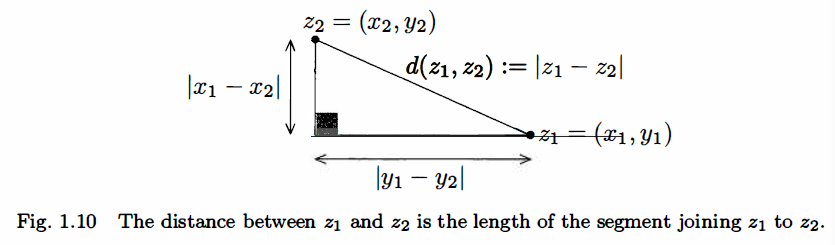
\includegraphics[width=0.9\textwidth]{./SaltChapter/fig-1-10}
\end{center}
\caption{복소수 $z_1$과 $z_2$사이의 거리는 $z_1$과 $z_2$를 잇는 선분의 길이다.}
\label{fig-1-10}
\end{figure}

복소수 덧셈의 기하학적 의미와 
삼각형의 두변의 길이의 합은 가장 큰 변의 길이보다 크다는 
유클리드 기하학의 유명한 결과를 이용하면
다음과 같이 복소수 절대값의 삼각 부등식을 얻는다.
$$
|z_1+z_2| \le |z_1|  + |z_2|, \quad z_1, z_2\in\mathbb C.
$$

그림 \ref{fig-1-11}을 보자.
이 삼각 부등식은 실수 $x_1, x_2, y_1, y_2$에 대한 코시-슈바르츠 부등식
$(x_1^2+y_1^2) (x_2^2+y_2^2) \ge (x_1x_2 + y_1y_2)^2$을 사용하여
확인할 수도 있다.


\begin{figure}[!h]
\begin{center}
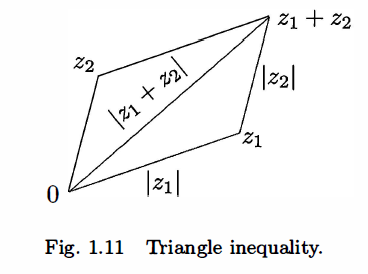
\includegraphics[width=0.5\textwidth]{./SaltChapter/fig-1-11}
\end{center}
\caption{삼각 부등식}
\label{fig-1-11}
\end{figure}

\begin{salt_exercise} \label{ex-1-22}
모든 복소수 $z_1, z_2\in \mathbb C$에 대하여
$|z_1-z_2| \ge \left| |z_1| - |z_2| \right|$을 증명하라.
\end{salt_exercise}

\begin{salt_exercise} \label{ex-1-23}
다음 집합을 복소평면에 나타내라.
\begin{itemize}
\item[(1)] $\left\{z\in\mathbb C\,:\, |z-(1-i)| = 2 \right\}$.
\item[(2)] $\left\{z\in\mathbb C\,:\, |z-(1-i)| < 2 \right\}$.
\item[(3)] $\left\{z\in\mathbb C\,:\, 1< |z-(1-i)| < 2 \right\}$.
\item[(4)] $\left\{z\in\mathbb C\,:\, \Re(z-(1-i)) = 3 \right\}$.
\item[(5)] $\left\{z\in\mathbb C\,:\, |\Im(z-(1-i))| < 2 \right\}$.
\item[(6)] $\left\{z\in\mathbb C\,:\, |z-(1-i)| = |z-(1+i)| \right\}$.
\item[(7)] $\left\{z\in\mathbb C\,:\, |z-(1-i)| + |z-(1+i)| = 2 \right\}$.
\item[(8)] $\left\{z\in\mathbb C\,:\, |z-(1-i)| + |z-(1+i)| < 3 \right\}$.
\end{itemize}
\end{salt_exercise}

\subsection{열린 원판, 열린 집합, 닫힌 집합, 콤팩트 집합}

주어진 점의 근방에 대한 집합을 다루기 위해 다음 정의들을 도입하는 것이 편리하다.
중심이 $z_0$이고 반지름이 $r>0$인 {\bf 열린 공/원판} $D(z_0,r)$은 
$D(z_0,r) :=\{ z\in\mathbb C \,:\, |z-z_0| <r \}$로 정의한다.

\begin{figure*}[!h]
\begin{center}
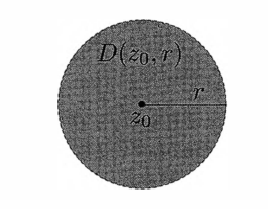
\includegraphics[width=0.3\textwidth]{./SaltChapter/fig-1-0-1}
\end{center}
\end{figure*}

$\mathbb C$의 부분집합 $U$에 속하는
모든 $z$에 대하여 $r_z>0$가 존재하여 $D(z,r_z)\subset U$를 만족하면
$U$를 {\bf 열린 집합}이라 한다.
다시 말하면, $U$의 어떤 점을 잡더라도 
주변의 모든 점이 $U$에 속할 수 있는 ``공간''이 존재한다.
예를 들면, 열린 원판 $D(z_0,r)$은 열린 집합이다.
따라서  $D(z_0,r)$를 열린 원판이라 부를 때 사용한 형용사 ``열린''은 적절해 보인다.
열린 집합의 예를 조금 더 만들어보자.
원환(annulus) $\mathbb A_r := \{ z\in\mathbb C\,:\, r<|z|<1\}$,
우측 반평면 $\mathbb H:= \{z\in\mathbb C\,:\, \Re(z)>0\}$는 모두 열린 집합이다.

열린 집합의 여집합에 특별한 이름을 붙여 ``닫힌 집합''이라 부르면 편리하다.
닫힌 집합은 수열의 수렴성의 관점에서 규정할 수도 있다.
집합 $F\subset \mathbb C$가 닫힌 집합이라는 것은
$F$에 속하는 복소수열 $(z_n)_{n\in\mathbb N}$이  $\mathbb C$에서 $L$로 수렴한다면
극한 $L$이 $F$에 속한다는 것과 동치이다.

$\mathbb C$의 부분집합 $S$의 모든 원소 $z$에 대하여
$|z|\le M$을 만족하는 $M>0$이 존재하면 $S$를 {\bf 유계}(bounded)라 한다.
그러면 $S$는 복소평면에서 충분히 큰 원판 내부에 속한다.

$\mathbb C$의 부분집합 $K$가 유계인 닫힌 집합이면 {\bf 콤팩트 집합}이라 한다.
콤팩트 집합에서 정의된 실변수 연속함수는 최대값과 최소값을 갖는다는
실해석학의 잘 알려진 결과를
앞으로 종종 사용할 것이다.

\subsection{수렴성과 연속성}












%===[salt] 2장
% !TEX root = ../notes_template.tex

\chapter{복소미분}

이 장에서는 다음 3가지 주제를 중점적으로 다룬다.

\begin{itemize}
\item[(1)] 복소미분의 정의:
즉, $\mathbb C$의 열린 부분집합 $U$에 정의된 함수 $f:U\to\mathbb C$와
$z_0\in U$가 주어졌을 때, ``$f$가 $z_0$에서 복소미분가능하고 복소미분값은 $f'(z_0)$이다''
라는 의미에 대하여 학습한다.
\item[(2)] 코시-리만 방정식: 
$\dfrac{\partial u}{\partial x} = \dfrac{\partial v}{\partial y}$와
$\dfrac{\partial u}{\partial y} = - \dfrac{\partial v}{\partial x}$.

이 방정식은 
복소미분가능함수 $f:U\to\mathbb C$의 실수부와 허수부 $u$, $v$가
만족하는 편미분방정식이다.

\begin{figure}[!h]
\begin{center}
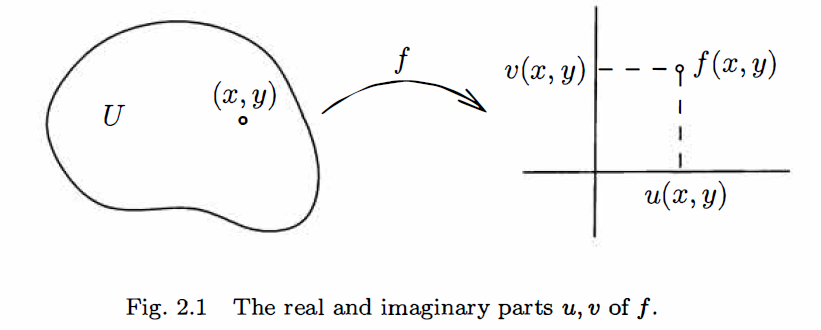
\includegraphics[width=0.6\textwidth]{./SaltChapter/fig-2-1}
\end{center}
\caption{$f$의 실수부와 허수부 $u$, $v$}
\label{fig-2-1}
\end{figure}

역으로, 어떤 열린집합 $U$의 모든 점에서 $C^1$-함수 $u, v$가 
코시-리만 방정식을 만족한다면 $f=u+iv$는 $U$에서 복소미분가능하다.

\item[(3)] 복소미분 $f'(z_0)$의 기하학적 의미:
국소적으로 보면, 함수 $f$는 $|f'(z_0)|$만큼 확대하면서
반시계방향으로 $\Arg(f'(z_0))$만큼 회전시키는 변환이다.
\end{itemize}

이 장에서는
열린집합에 정의된 복소미분가능함수가 
코시-리만 방정식을 만족할 필요충분조건(다소 덜 엄밀한 방식으로)에 대하여
중점적으로 다룬다.

\section{복소 미분가능성}

\begin{salt_definition}\label{def-2-1}
\
\begin{itemize}
\item[(1)] $U$가 $\mathbb C$의 열린 부분집합, $f: U\to \mathbb C$, $z_0\in U$라 하자.
다음 식을 만족하는 복소수 $L$이 존재하면, $f$가 $z_0$에서 {\bf 복소미분가능}이라 한다.
\[
\lim_{z\to z_0} \dfrac{f(z) - f(z_0)}{z - z_0} = L.
\]
즉, 임의의 $\epsilon>0$에 대하여 $\delta>0$가 존재하여,
$z\in U$, $0<|z-z_0|<\delta$이면 
\[
\left| \dfrac{f(z) - f(z_0)}{z - z_0} - L\right| < \epsilon
\]
을 만족한다.

극한값  $L$은 유일하게 결정되며 다음과 같이 나타낸다.
\[
f'(z_0) \quad\text{또는}\quad \dfrac{df}{dz}(z_0).
\]

\item[(2)] 열린집합 $U$에 정의된 함수 $f:U\to\mathbb C$가 $U$의 모든 점에서
복소미분가능하면 복소해석적(holomorphic\footnote{
``holomorphic''이라는 용어는 전체(entire)를 뜻하는 그리스어 ``holo''와
``모양(form)'' 또는 ``형세(apprearance)''을 나타내는 ``morphe''에서 파생되었다.
})이라 부른다.
\item[(3)] 복소수 $\mathbb C$ 전체에서 복소해석적이면 
전해석(entire) 함수라 부른다. 즉, $f$의 정의역이 복소수 $\mathbb C$ 전체이고
$\mathbb C$에서 복소해석적임을 의미한다.
\end{itemize}
\end{salt_definition}

전해석 함수의 간단한 예를 살펴보자.

\begin{salt_example} \label{example-2-1}
함수 $f:\mathbb C \to \mathbb C$를 $f(z) = z^2$ ($z\in\mathbb C$)라 정의하자.
그러면 $f$가 전해석 함수임을 보일 수 있다.
$z$가 $z_0$의 근방에 있을 때,
\[
\dfrac{f(z) - f(z_0)}{z - z_0} = \dfrac{z^2 - z_0^2}{z-z_0} = z + z_0 
\approx 2z_0
\]
이므로, $f'(z_0) = 2z_0$라고 추측할 수 있다.
이를 증명해 보자.
$z\ne z_0$에 대하여
\[
\left| \dfrac{f(z) - f(z_0)}{z - z_0} - 2z_0 \right|
= \left| \dfrac{z^2 - z_0^2}{z-z_0} - 2z_0 \right| 
= |z+z_0-2z_0| = |z-z_0|.
\]
따라서 $z$가 $z_0$에 충분히 가까우면
좌변을 원하는 만큼 작은 값으로 만들 수 있다.
$\epsilon>0$이라 하자.
$\delta:=\epsilon>0$으로 잡으면,
$z\in\mathbb C$가 $0<|z-z_0| <\delta$를 만족할 때마다
\[
\left| \dfrac{f(z) - f(z_0)}{z - z_0} - 2z_0 \right|
= |z-z_0| <\delta = \epsilon.
\]
결론적으로 $f'(z_0) = 2z_0$가 성립한다.
$z_0\in\mathbb C$를 임의로 선택할 수 있으므로,
$f$는 $\mathbb C$ 전체에서 복소해석적이고,
전해석 함수가 된다. 이상에서 다음 결론을 얻는다.
\[
\dfrac{d}{dz} z^2 = 2z, \quad z\in \mathbb C.
\]
\end{salt_example}

다른 방향으로, 이제 복소미분가능하지 않은 함수의 예를 보자.

\begin{salt_example} \label{example-2-2}
함수 $g:\mathbb C \to \mathbb C$를 $g(z) = \bar z$ ($z\in\mathbb C$)라 정의하자.
그러면 $g$는 어떤 점에서도 복소미분이 불가능함을 보일 수 있다.
$g$가 $z_0\in\mathbb C$에서 복소미분가능하다고 하자.
$\epsilon:=\frac12 >0$라 하면, $\delta>0$이 존재하여
$z$가 $0<|z-z_0|<\delta$를 만족할 때마다 
\[
\left| \dfrac{g(z)-g(z_0)}{z-z_0} - g'(z_0) \right| 
= \left| \dfrac{\bar z - \overline{z_0}}{z-z_0} - g'(z_0) \right| 
<\epsilon
\]
이 성립한다.

그림 \ref{fig-2-2}의 왼쪽을 보자.
위의 식에 따르면,
중심이 $z_0$이고 반지름이 $\delta$인 뚫린 원판(punctured disk)에 $z$가 속할 때마다
부등식이 성립함을 보장한다.
이제 그림의 뚫린 원판 내부에 $z_0$의 위쪽과 오른쪽에 한점씩을 선택하자.
이 점들을 부등식에 넣어보면, $g'(z_0)$는 각각 $-1$과 $1$을 중심으로 하고 반지름 $1/2$인
원판 내부에 속해야 한다.
그림 \ref{fig-2-2}의 오른쪽을 참고하면, 두 원판은 겹치치 않으므로 모순이 되어 증명이 끝난다.
아래에서 좀 더 자세히 살펴보자.

\begin{figure}[!h]
\begin{center}
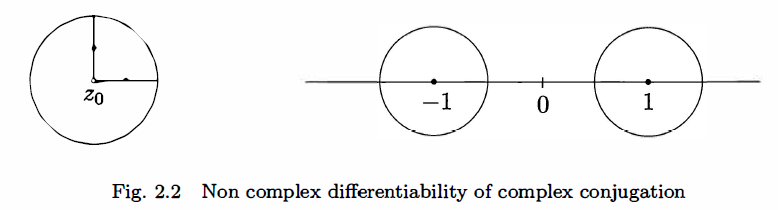
\includegraphics[width=0.8\textwidth]{./SaltChapter/fig-2-2}
\end{center}
\caption{켤레복소수 함수의 미분 불가능성}
\label{fig-2-2}
\end{figure}

$z=z_0+ \dfrac\delta2$로 잡으면, $0<|z-z_0|<\delta$이므로
\begin{equation} \label{eq-2-1}
\left| \dfrac{\bar z - \overline{z_0}}{z-z_0} - g'(z_0) \right| 
= \left| \dfrac{\delta/2}{\delta/2} - g'(z_0) \right| 
= | 1 - g'(z_0)| < \epsilon.
\end{equation}
한편, $z=z_0+ i\dfrac\delta2$로 잡으면, $0<|z-z_0|<\delta$이므로
\begin{equation} \label{eq-2-2}
\left| \dfrac{\bar z - \overline{z_0}}{z-z_0} - g'(z_0) \right| 
= \left| \dfrac{-\delta/2}{\delta/2} - g'(z_0) \right| 
= | 1 + g'(z_0)| < \epsilon.
\end{equation}
식 \eqref{eq-2-1}과 \eqref{eq-2-2}로부터
\[
2 = | 1- g'(z_0) + 1+ g'(z_0)|
\le |1-g'(z_0)| + |1+g'(z_0)| < \epsilon + \epsilon 
= 2\epsilon = 2\cdot\dfrac12 = 1
\]
이 되어 모순이다.
따라서 $g$는 $z_0$에서 복소미분가능하지 않다.
\end{salt_example}

\begin{salt_exercise} \label{ex-2-1}
모든 $z\in\mathbb C$에 대하여 $f(z) = |z|^2$로 정의된
함수 $f:\mathbb C \to \mathbb C$는 $0$에서 복소미분가능하며
$f'(0)=0$임을 보여라.
나중에 (연습문제 \ref{ex-2-9}에서) $f$는 $0$이 아닌 모든 점에서 복소미분 불가능함을 보일 것이다.
\end{salt_exercise}

\begin{salt_exercise} \label{ex-2-2}
영역 $D$에 정의된 함수 $f:D\to \mathbb C$가 복소해석적이라 하자.
$D^* := \{ z\in \mathbb C \,:\, \bar z \in D\}$에 
함수 $f^*:D^* \to \mathbb C$를 $f^*(z) = \overline{f(\bar  z)}$ ($z\in D^*$)로
정의하면 $f^*$가  $D^*$에서 복소해석적임을 증명하라.
\end{salt_exercise}

복소미분 가능성에 대한 다음 변형은 복소미분에 대한 기본 공식을 증명하는 데 유용하게 사용된다.
대략적으로 말하면, 복소미분가능함수 $f$가 $z_0$에서 미분값 $L$을 갖는다면
$f(z)-f(z_0) - L\cdot (z-z_0)$가 $z-z_0$보다 $0$으로 빠르게 수렴함을 뜻한다.

\begin{salt_lemma} \label{lemma-2-1}
$U$가 $\mathbb C$의 열린 집합이고, $z_0\in U$, $f:U\to\mathbb C$라 하면,
다음은 동치이다.
\begin{itemize}
\item[(1)] $f$가 $z_0$에서 복소미분가능하며, $f'(z_0)=L$이다.
\item[(2)] 양수 $r>0$과  $D(z_0,r):=\{z\in\mathbb C\,:\, |z-z_0|<r\}$에 정의된
함수  $h:D(z_0,r)\to \mathbb C$가 존재하여 다음을 만족한다.
\begin{itemize}
\item[(a)] $|z-z_0|<r$에 대하여 $f(z)=f(z_0) + (L+h(z))(z-z_0)$이고,
\item[(b)] $\lim\limits_{z\to z_0} h(z)=0$.
\end{itemize}
\end{itemize}
\end{salt_lemma}

{\bf 증명}

(2)$\Rightarrow$(1):
$z\in D(z_0,r)\setminus \{z_0\}$에 대하여 (a)의 식을 재정리하면,
\[
\dfrac{f(z) - f(z_0)}{z - z_0} - L = h(z) \stackrel{z\to z_0}{\longrightarrow} 0
\]
이므로 $f$는 $z_0$에서 복소미분가능하며 $f'(z_0)=L$이다.

(1)$\Rightarrow$(2):
이제 $f$가 $z_0$에서 복소미분가능하다고 가정하자. 
그러면 $\delta_1>0$이 존재하여 \\
$0<|z-z_0|<\delta_1$, $z\in U$이면 
\[
\left|  \dfrac{f(z) - f(z_0)}{z - z_0}  - f'(z_0) \right| < 1
\]
이다.
$r:=\delta_1$으로 설정하고 함수 $h:D(z_0,r) \to \mathbb C$를 
\[
h(z) = \begin{cases}
\dfrac{f(z) - f(z_0)}{z - z_0} - f'(z_0), & z\ne z_0, \\
0, & z= z_0
\end{cases}
\]
로 정의하자.
그러면 $|z-z_0|<r$일 때
$f(z) = f(z_0) + \left( f'(z_0) + h(z)\right) (z - z_0)$가 성립한다.
이제 (b)를 보이기 위해 $\epsilon>0$이 주어졌다고 하자.
$0<|z-z_0|<\delta$이면
\[
\left|  \dfrac{f(z) - f(z_0)}{z - z_0}  - f'(z_0) \right| \ \left( = |h(z) - 0| \right) < \epsilon
\]
이 되는 $\delta>0$를 잡을 수 있다 ($r$보다 작다는 조건도 만족하도록).
이로써 (a), (b)를 모두 성립함을 알 수 있다. \hfill $\square$

\begin{salt_exercise} \label{ex-2-3}
영역 $D\subset \mathbb C$에 정의된 함수 $f:D\to \mathbb C$가 
$z_0\in D$에서 복소미분가능하다면 $f$는 $z_0$에서 연속임을 보여라.
나중에 우리는 $f$가 $D$에서 복소해석적이면, 
실제로 $D$의 모든 점에서 무한번 미분가능함을 보일 것이다.
\end{salt_exercise}

보조정리 \ref{lemma-2-1}을 이용하여 다음을 쉽게 얻을 수 있다.

\begin{salt_prop}\label{prop-2-1}
$U$가 $\mathbb C$의 열린 부분집합이고,
$f,g: U\to \mathbb C$가 $z_0\in U$에서 복소미분가능함수이면
다음이 성립한다.
\begin{itemize}
\item[(1)] $f+g$는 $z_0$에서 복소미분가능하고
$(f+g)'(z_0) = f'(z_0) = g'(z_0)$이다. \\
(함수 $f+g:U\to\mathbb C$는 $z\in U$에 대하여 $(f+g)(z) = f(z)+g(z)$로 정의한다)
\item[(2)] $\alpha\in\mathbb C$에 대하여 $\alpha\cdot f$는 $z_0$에서 복소미분가능하고
$(\alpha\cdot f)'(z_0) = \alpha f'(z_0)$이다. \\
(함수 $\alpha \cdot f:U\to\mathbb C$는 $z\in U$에 대하여 
$(\alpha \cdot f)(z) = \alpha f(z)$로 정의한다)
\item[(3)] $fg$는 $z_0$에서 복소미분가능하고
$(fg)'(z_0) = f'(z_0)g(z_0) + f(z_0)g'(z_0)$이다.\\
(함수 $fg:U\to\mathbb C$는 $z\in U$에 대하여 
$(fg)(z)= f(z)g(z)$로 정의한다)
\end{itemize}
\end{salt_prop}

\begin{salt_remark}\label{remark-2-1}
$U$가 $\mathbb C$의 열린 부분집합이고,
$\Hol(U)$가 $U$에 정의된 복소해석 함수의 집합이라고 하자.
그러면 위 명제로부터 $\Hol(U)$가 점별 연산에 대하여 복소 벡터공간을 이룸을 알 수 있다.
한편 위 명제의 세번째 내용은 두 복소해석 함수의 점별 곱셈은 다시 복소해석적임을 뜻한다.
따라서 $\Hol(U)$는 점별 덧셈과 곱셈에 대하여
환(ring) 구조를 갖는다.
\end{salt_remark}

\begin{salt_example}\label{example-2-3}
$f(z):=z$ ($z\in \mathbb C$)에 대하여 $f'(z)=1$임을 쉽게 보일 수 있다.
두 복소해석함수의 점별 곱셈에 대한 복소미분 규칙을 이용하면,
수학적 귀납법으로 모든 $n\in \mathbb N$에 $z\mapsto z^n$이 전해석함수이고
\[
\dfrac{d}{dz} z^n = nz^{n-1}
\]
임을 알 수 있다.
특히, 모든 다항식은 전해석함수이다.
\end{salt_example}

\begin{salt_exercise} \label{ex-2-4}
명제 \ref{prop-2-1}을 증명하라.
\end{salt_exercise}


\begin{salt_exercise} \label{ex-2-5}
$\mathbb D = \{ z\in\mathbb C \,:\, |z|<1 \}$이고
$\Hol(\mathbb D)$가 $\mathbb D$에 정의된 복소해석함수의 점별 연산으로 이루어진
복소 벡터공간이라 하자.  $\Hol(\mathbb D)$는 유한차원인가?
\end{salt_exercise}


\begin{salt_exercise} \label{ex-2-6}
$U$가 $\mathbb C$의 열린 부분집합이고,
$U$에 정의된 복소해석함수 $f:U\to \mathbb C$가 
$z\in U$에 대하여 $f(z)\ne 0$라고 하자.
\[
\dfrac 1f : U \to \mathbb C \text{ 를 }
\left( \dfrac 1f \right) (z) = \dfrac 1{f(z)} \text{ 로 정의할 때 }
\]
복소해석함수가 되며 복소미분이 다음과 같음을 보여라.
\[
\left( \dfrac 1f \right)' (z) = - \dfrac{f'(z)}{(f(z))^2} \quad (z\in U).
\]
\end{salt_exercise}

\begin{salt_exercise} \label{ex-2-7}
$\mathbb C\setminus \{0\}$에서 정수 $m\in\mathbb Z$에 대하여
$\dfrac d{dz} z^m = mz^{m-1}$임을 증명하라.
\end{salt_exercise}

실수에서 정의된 합성함수의 미분에 대한 연쇄법식과 같이
복소해석함수의 합성에 대해서도 유사한 연쇄법식이 존재한다.

\begin{salt_prop}[연쇄법칙] \label{prop-2-2} 
\ 
\begin{itemize}
\item[(1)] $D_f$, $D_g$가 복소평면 위의 영역이고,
\item[(2)] $f:D_f \to \mathbb C$가 $D_f$에서 복소해석적이고,
\item[(3)] $g:D_g \to \mathbb C$가 $D_g$에서 복소해석적이고,
\item[(4)] $f(D_f) \subset D_g$일 때,
\end{itemize}
$z\in D_f$에 대하여 $(g\circ f)(z) = g(f(z))$로 정의된
합성함수 $g\circ f : D_f \to \mathbb C$는 $D_f$에서
복소해석함수이고, 
모든 $z\in D_f$에 대하여 $(g\circ f)'(z) = g'(f(z))f'(z)$이다.
\end{salt_prop}

\begin{figure}[!h]
\begin{center}
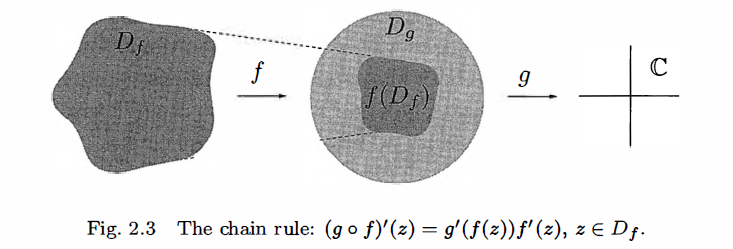
\includegraphics[width=0.7\textwidth]{./SaltChapter/fig-2-3}
\end{center}
\caption{연쇄법칙: $z\in D_f$에 대하여 $(g\circ f)'(z) = g'(f(z))f'(z)$}
\label{fig-2-3}
\end{figure}

{\bf 증명}

$z_0\in D_f$라 하자. 그러면 $f(z_0)\in D_g$이다.
$f$가 $z_0$의 근방에서 복소미분가능하고
$g$가 $f(z_0)$의 근방에서 복소미분가능하므로,
원판 $D(z_0, r_f)\subset D_f$와 $D(f(z_0), r_g) \subset D_g$에 각각 정의된
함수 $h_f$와 $h_g$가 존재하여 다음을 만족한다.
\begin{gather*}
f(z) - f(z_0) = (f'(z_0)+h_f(z))(z-z_0), \\
g(w) - g(f(z_0)) = (g'(f(z_0)) + h_g(w))(w-f(z_0)),
\end{gather*}
또한
\[
\lim_{z\to z_0} h_f(z)=0, \quad
\lim_{w\to f(z_0)} h_g(w)=0.
\]
$f$가 $z_0$에서 연속이므로
$z$가 $z_0$에 가까워질 때 $w:=f(z)$도 $f(z_0)$에 가까워지므로
$z\ne z_0$이고 $z_0$에 가까워지면, 다음 식을 얻는다.
\[
\dfrac{(g\circ f)(z) - (g\circ f)(z_0)}{z-z_0} 
= (g'(f(z_0)) + h_g(f(z)))(f'(z_0) + h_f(z)).
\]
이로써 증명이 끝난다. \hfill $\square$

\begin{salt_example}\label{example-2-4}
연습문제 \ref{ex-2-7}로부터
\[
\dfrac d{dz} \left(\dfrac 1z \right) = - \dfrac 1{z^2}, \quad
z\in \mathbb C \setminus \{0\}
\]
임을 알지만, 복소미분 정의로부터도의 쉽게 유도할 수 있다. 왜냐 하면,
$z_0\in \mathbb C \setminus \{0\}$에 대하여 다음 식이 성립하기 때문이다.
\[
\dfrac{\dfrac 1z - \dfrac1{z_0}}{z-z_0} = \dfrac{z_0 - z}{zz_0(z-z_0)}
= \dfrac{-1}{zz_0} \stackrel{z\to z_0}{\longrightarrow} - \dfrac 1{z_0^2}.
\] 
\begin{figure}[!h]
\begin{center}
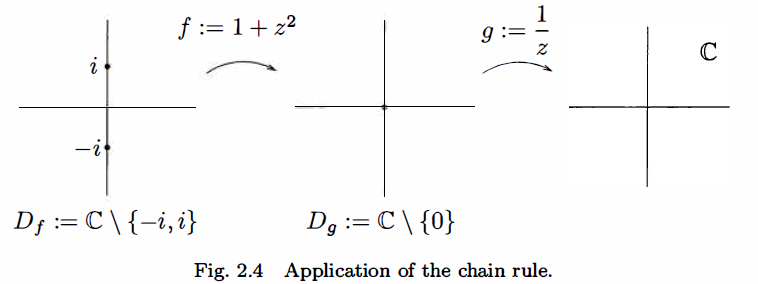
\includegraphics[width=0.7\textwidth]{./SaltChapter/fig-2-4}
\end{center}
\caption{연쇄법칙의 응용}
\label{fig-2-4}
\end{figure}
이제 $D_f:=\mathbb C \setminus \{-i,i\}$에 정의된 함수 $f:= 1+z^2$와
$D_g:=\mathbb C \setminus \{0\}$에 정의된 함수 $g:=1/z$를 생각하자.
$f(D_f) \subset D_g$이 성립함이 명확하므로 연쇄법식에 의해
$\mathbb C \setminus \{-i, i\}$에서
\[
\dfrac d{dz} \left( \dfrac 1{1+z^2} \right) = - \dfrac 1{(1+z^2)^2}\cdot 2z
= - \dfrac{2z}{(1+z^2)^2}.
\]
\end{salt_example}

\begin{salt_exercise} \label{ex-2-8}
$\exp z$가 전해석함수이고 $\exp' z = \exp z$라 가정하고(나중에 증명할 예정이다),
\[
z \mapsto \exp \left( - \dfrac{1+z}{1-z} \right)
\]
가 단위 원판 $\mathbb D := \{ z \in \mathbb C \,:\, |z|<1 \}$에서
복소미분가능함수임을 보이고, 미분을 구하라.
\end{salt_exercise}

\section{코시-리만 방정식}

이제 이 장에서 가장 중요한 결과를 증명해보자.
간략히 말하면, 함수  $f=u+iv$가 복소미분가능하다는 것은
실수부 $u$와 허수부 $v$ ($\mathbb R^2$의 열린 부분집합에 정의된 실함수로 볼 수 있는)가
코시-리만(Cauchy-Riemann) 방정식이라 불리는 편미분 방정식을 만족함과 동치이다. 

\begin{figure*}[!h]
\begin{center}
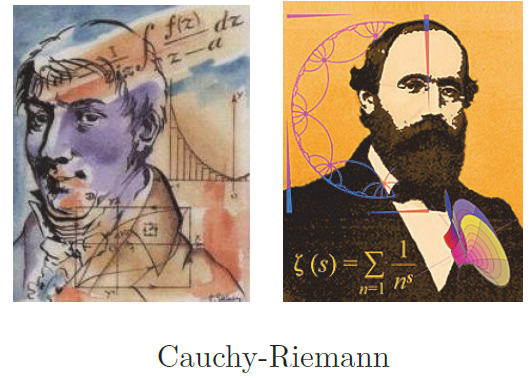
\includegraphics[width=0.4\textwidth]{./SaltChapter/fig-2-0-1} \\
{코시-리만(Cauchy-Riemann)}
\end{center}
%== [salt]?? 캡션을 넣으면 번호가 자동부여?
%\caption{코시-리만(Cauchy-Riemann)}
\end{figure*}


$\mathbb C$의 열린 부분집합 $U$에 정의된
함수 $f:U\to \mathbb C$를 생각하자.
그러면 임의의 점 $(x,y)\in U$에 대하여 $f(x+iy)\in\mathbb C$이고,
$f(x+iy)$의 실수부 $u(x,y)$와 허수부 $v(x,y)$를 그림 \ref{fig-2-5}와 같이 볼 수 있다.

\begin{figure}[!h]
\begin{center}
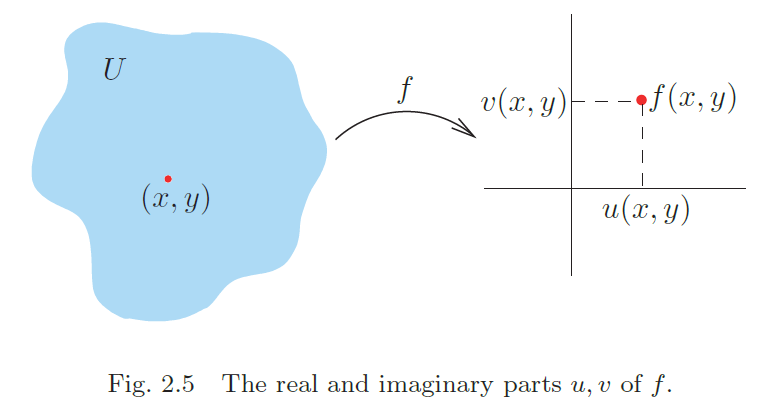
\includegraphics[width=0.6\textwidth]{./SaltChapter/fig-2-5}
\end{center}
\caption{$f$의 실수부 $u$와 허수부 $v$}
\label{fig-2-5}
\end{figure}

점 $(x,y)$가 변하면 $f(x+iy)$도 변하며, $u(x,y)$와 $v(x,y)$도 마찬가지다.
이런 방법으로, $f$와 연관된 실함수를 얻는다.
\begin{align*}
u:U\to \mathbb R, & U \ni (x,y) \mapsto \Re(f(x+iy)) =: u(x,y), \\
v:U\to \mathbb R, & U \ni (x,y) \mapsto \Im(f(x+iy)) =: v(x,y). \\
\end{align*}

이 장의 첫번째 결과는 코시-리만 방정식이 복소미분가능성에 대한 필요조건이라는 것이며
이는 정리 \ref{thm-2-1}에서 증명할 것이다. 
즉, $f$가 $(x_0, y_0) \in U$에서 복소미분가능하다면,

\begin{center}
$(x_0, y_0)$에서
\fbox{
$\dfrac{\partial u}{\partial x} =  \dfrac{\partial v}{\partial y}$ 이고
$\dfrac{\partial u}{\partial y} = - \dfrac{\partial v}{\partial x}$.
}
\end{center}

이를 이 방정식을 코시-리만 방정식이라 부른다.
따라서 복소미분가능함수는 이 방정식을 만족한다.
다시 말하면, 복소함수의 실수부와 허수부가 어떤 점에서 이 방정식을 만족하지 않는다면,
그 점에서 복소미분가능하지 않음을 알 수 있다.
여기서 예제 하나를 보자. 앞에서 우리는 $\epsilon-\delta$를 이용한 복소미분의 정의로부터
직접 계산하여 $z\mapsto \bar z$가 복소평면위의 어느 점에서도 미분가능하지 않음을 보였다.
예제 \ref{example-2-2}를 다시 살펴보자.

\begin{salt_example} \label{example-2-5}
$g(z) = \bar z$ ($z\in \mathbb C$)로 정의된 함수 $g:\mathbb C \to \mathbb C$에 대하여
\begin{align*}
u(x,y) &=\Re(g(x+iy)) = \Re(x-iy) = x, \\
v(x,y) &= \Im(g(x+iy)) = \Im(x-iy) = -y
\end{align*}
이므로
\[
\dfrac{\partial u}{\partial x} = 1 \ne -1 = \dfrac{\partial v}{\partial y}.
\]
이 결과는 코시-리만 방정식이 어떤 점에서도 성립하지 않음을 의미한다.
따라서 $g$가 어떤 점에서도 복소미분가능하지 않다는 이전 결과를 쉽게 얻을 수 있다.
\end{salt_example}


코시-리만 방정식이 복소미분가능성에 대한 필요조건이라는 것을 증명하기에 앞서
이 절에서 증명할 두번째로 중요한 결과로
열린집합에서 복소해석적일 충분조건으로서
코시-리만 방정식에 대하여 언급하고자 한다.
좀 더 정확히 말하면, 
열린집합 $U$에 정의된 함수 $u,v: U\to \mathbb R$가 
$U$에서 연속미분가능하고 (이변수 실함수로서),
$U$의 모든 점에서 코시-리만 방정식을 만족하면,
$u$, $v$로부터 $f(x+iy):=u(x,y) + iv(x,y)$ $(x,y)\in U$로 정의하여 만든
($u$, $v$가 $f$의 실수부와 허수부가 되도록)
새로운 복소함수 $f:U\to\mathbb C$는 복소해석적이다.
이 중요한 결과로부터 우리는
$\epsilon-\delta$ 정의를 이용하는 매우 긴 증명을 통하지 않고
주요 함수의 복소미분가능성을 확인할 수 있다.
예제를 살펴보자.

\begin{salt_example} \label{example-2-6}
뚫린 평면 $\mathbb R^2 \setminus \{(0,0)\}$에서 
\[
u(x,y) := \dfrac{x}{x^2+y^2}, \quad
v(x,y) := \dfrac{-y}{x^2+y^2}, \quad (x,y)\ne(0,0)
\]
로 정의된 함수 
$u$, $v$를 생각하자.
그러면 다음 편미분을 얻는다.
\begin{align*}
\dfrac{\partial u}{\partial x} &= \dfrac{1\cdot(x^2+y^2)-x\cdot 2x}{(x^2+y^2)^2}
= \dfrac{y^2-x^2}{(x^2+y^2)^2}, \\
\dfrac{\partial u}{\partial y} &= \dfrac{-x\cdot 2y}{(x^2+y^2)^2}
= \dfrac{-2xy}{(x^2+y^2)^2}, \\
\dfrac{\partial v}{\partial x} &= \dfrac{2xy}{(x^2+y^2)^2}, \quad
\dfrac{\partial v}{\partial y} = \dfrac{y^2-x^2}{(x^2+y^2)^2}.
\end{align*}
당연히 $\mathbb R^2$에서 $(x,y) \mapsto (x^2+y^2)^2, y^2-x^2, \pm 2xy$는 
연속함수이고, $(x^2+y^2)^2$은 $\mathbb R^2 \setminus \{(0,0)\}$에서 
$0$이 아니다.
따라서 $u$, $v$는 $\mathbb R^2 \setminus \{(0,0)\}$에서 
연속미분가능하다.
또한 코시-리만 방정식이 성립한다. 
결론적으로 $f:=u+iv$는 $\mathbb C\setminus\{0\}$에서 
복소해석적이다.
실제로 위에서 정의한 $f$는 다름 아닌 분수함수 $z\mapsto 1/z$이다.
\[
f=u+iv= \dfrac x{x^2+y^2}+i\left(\dfrac{-y}{x^2+y^2}\right)
= \dfrac{x-iy}{x^2+y^2} = \dfrac{\bar z}{|z|^2} = \dfrac{\bar z}{z \bar z}
= \dfrac  1z, \quad z\ne 0.
\]
\end{salt_example}

\begin{salt_theorem}\label{thm-2-1}
$U$가 $\mathbb C$의 열린 부분집합이고
$f:U\to \mathbb C$가 $z_0=x_0+iy_0\in U$에서 복소미분가능하다고 하자.
그러면 함수
\begin{align*}
(x,y) \mapsto u(x,y) & := \Re(f(x+iy)): U\to \mathbb R,
(x,y) \mapsto v(x,y) & := \Im(f(x+iy)): U\to \mathbb R
\end{align*}
는 $(x_0, y_0)$에서 미분가능하고 다음을 만족한다.
\begin{equation} \label{eq-2-3}
\dfrac{\partial u}{\partial x}(x_0,y_0) = \dfrac{\partial v}{\partial y}(x_0,y_0),
\quad
\dfrac{\partial u}{\partial y}(x_0,y_0) = - \dfrac{\partial u}{\partial x}(x_0,y_0),.
\end{equation}
\end{salt_theorem}

{\bf 증명}
(중명의 아이디어는 쉽다. 단지 $(x,y)$를 $(x_0, y_0)$에 가까이 보낼 때
첫번째로 $y$를 $y_0$로 고정하는 방법으로 하고 그 다음에 
$x$를 $x_0$로 고정하는 방법을 사용한 후 각 결과를 살펴본다.
그림 \ref{fig-2-6}을 참고하라.)

\begin{figure}[!h]
\begin{center}
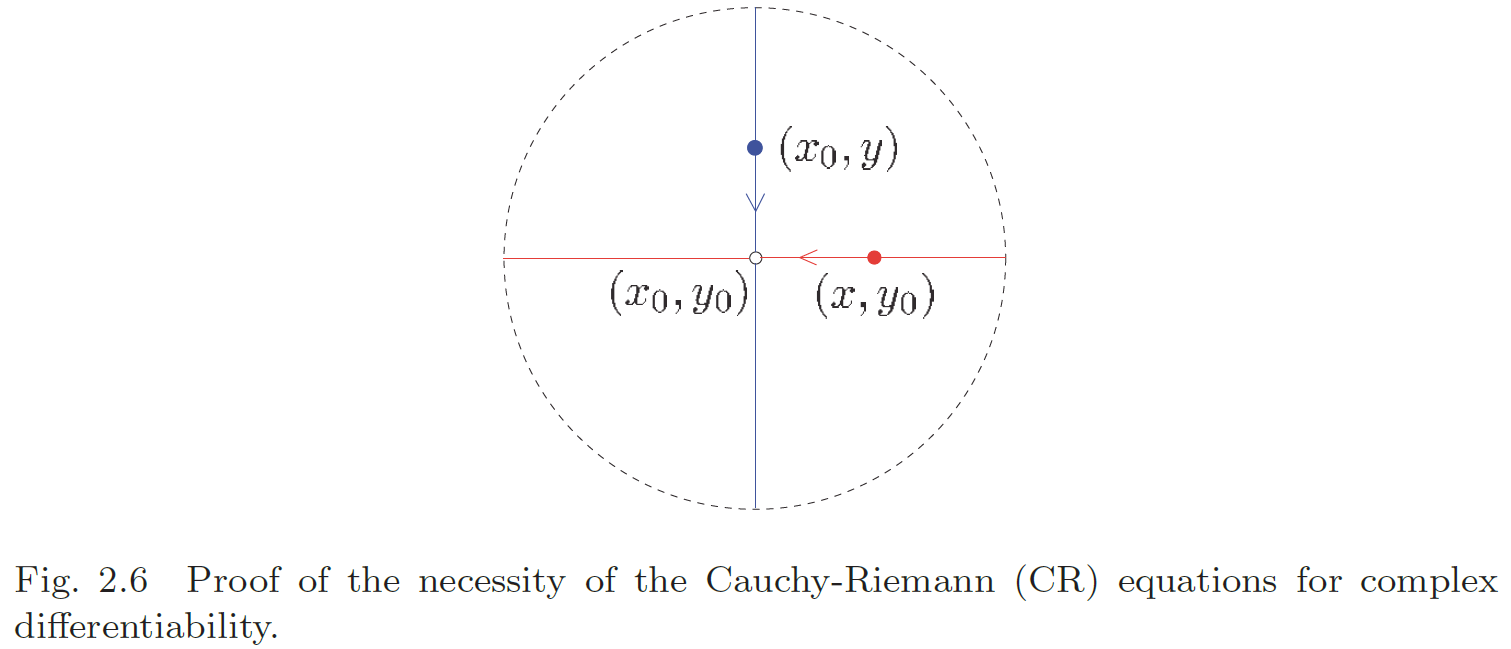
\includegraphics[width=0.9\textwidth]{./SaltChapter/fig-2-6}
\end{center}
\caption{복소미분가능성에 대하여 코시-리만(CR) 방정식이 필요조건임을 증명}
\label{fig-2-6}
\end{figure}

$z_0 = (x_0, y_0)\in U$라 하자.
$\epsilon>0$에 대하여, 
$0<|z-z_0|<\delta$일 때 $z\in U$에 대하여
\begin{equation}\label{eq-2-4}
\left| \dfrac{f(z)-f(z_0)}{z-z_0} - f'(z_0) \right| < \epsilon
\end{equation}
을 만족하는 $\delta >0$가 존재한다.

{\bf 단계 1:}
$\dfrac{\partial u}{\partial x}(x_0,y_0)$가 존재하고 $\Re(f'(z_0))$와 같음을 증명하자.

$0<|x-x_0|<\delta$를 만족하는 $x\in\mathbb R$에 대하여 $z:=x+iy_0$라고 하자.
그러면 $z-z_0 = x-x_0$를 만족하므로
$0<|z-z_0| = |x-x_0| < \delta$가 된다.
이제 다음을 식 \eqref{eq-2-4}로부터 얻을 수 있다. 
\begin{align*}
\left| \dfrac{u(x,y_0) - u(x_0, y_0)}{x-x_0} - \Re(f'(z_0)) \right| 
&= \left| \Re\left(\dfrac{f(x+iy_0)-f(x_0+iy_0)}{x-x_0}\right) - \Re(f'(z_0)) \right| \\
&= \left| \Re\left(\dfrac{f(z)-f(z_0)}{z-z_0}\right) - \Re(f'(z_0)) \right| \\
&\le \left| \dfrac{f(z)-f(z_0)}{z-z_0} - f'(z_0) \right| < \epsilon 
\end{align*}
따라서 편미분 결과는 다음과 같다.
\begin{align*}
\dfrac{\partial u}{\partial x}(x_0, y_0) 
&= \lim_{x\to x_0} \dfrac{u(x,y_0) - u(x_0, y_0)}{x-x_0} \\
&= \Re(f'(z_0)).
\end{align*}

{\bf 단계 2:}
$\dfrac{\partial v}{\partial x}(x_0, y_0)  = \Im(f'(z_0))$를 증명하자.

단계 1에서 사용한 표기법을 적용하여 다음을 보일 수 있다.
\begin{align*}
\left| \dfrac{v(x,y_0) - v(x_0, y_0)}{x-x_0} - \Im(f'(z_0)) \right| 
&= \left| \Im\left(\dfrac{f(x+iy_0)-f(x_0+iy_0)}{x-x_0}\right) - \Im(f'(z_0)) \right| \\
&= \left| \Im\left(\dfrac{f(z)-f(z_0)}{z-z_0}\right) - \Im(f'(z_0)) \right| \\
&\le \left| \dfrac{f(z)-f(z_0)}{z-z_0} - f'(z_0) \right| < \epsilon 
\end{align*}
따라서
$\dfrac{\partial v}{\partial x}(x_0, y_0) 
= \lim\limits_{x\to x_0} \dfrac{v(x,y_0) - v(x_0, y_0)}{x-x_0} 
= \Im(f'(z_0))$. 종합하면,
\begin{equation}\label{eq-2-5}
f'(z_0) = \dfrac{\partial u}{\partial x}(x_0, y_0)
+ i \dfrac{\partial v}{\partial x}(x_0, y_0).
\end{equation}

{\bf  단계 3:}
$\dfrac{\partial u}{\partial y}(x_0, y_0)  = - \Im(f'(z_0))$를 증명하자.

$0<|y-y_0|<\delta$를 만족하는 $y\in\mathbb R$에 대하여 $z:=x_0+iy$라고 하자.
그러면 $z-z_0 = i(y-y_0)$를 만족하므로
$0< |z-z_0| = |y-y_0| <\delta$가 된다.
이제 실수 $a$, $b$에 대하여
$\Re(a+ib) = \Im(i(a+ib))$가 성립함을 이용하면 다음을 얻는다.
\begin{align*}
\left| \dfrac{u(x_0,y) - u(x_0, y_0)}{y-y_0} + \Im(f'(z_0)) \right| 
&= \left| \dfrac{\Im(i(f(z)-f(z_0)))}{y-y_0} + \Im(f'(z_0)) \right| \\
&= \left| \Im\left(-\dfrac{f(z)-f(z_0)}{z-z_0} +f'(z_0) \right) \right| \\
&\le \left| \dfrac{f(z)-f(z_0)}{z-z_0} - f'(z_0) \right| < \epsilon .
\end{align*}
따라서 편미분은
$$
\dfrac{\partial u}{\partial y}(x_0, y_0) 
= \lim\limits_{y\to y_0} \dfrac{u(x_0,y) - u(x_0, y_0)}{y-y_0} 
= -\Im(f'(z_0)).
$$
단계 2에서 다음 식을 얻은 것을 기억하면
$$
\dfrac{\partial v}{\partial x}(x_0, y_0) 
= \Im(f'(z_0)),
$$
이로부터 코시-리만 방정식의 두개 중 하나를 얻는다. 즉,
$$
\dfrac{\partial u}{\partial y}(x_0, y_0) = - \dfrac{\partial v}{\partial x}(x_0, y_0).
$$

{\bf 단계 4:}
$\dfrac{\partial v}{\partial y}(x_0, y_0)  = \Re(f'(z_0))$를 증명하자.

단계 3에서 사용한 표기법을 적용하고,
실수 $a$, $b$에 대하여
$\Im(a+ib) = -\Re(i(a+ib))$가 성립함을 이용하면 다음을 얻는다.
\begin{align*}
\left| \dfrac{v(x_0,y) - v(x_0, y_0)}{y-y_0} - \Re(f'(z_0)) \right| 
&= \left| -\Re\left( i\dfrac{f(z)-f(z_0)}{y-y_0}\right) - \Re(f'(z_0)) \right| \\
&\le \left| -i\dfrac{f(z)-f(z_0)}{y-y_0} - f'(z_0) \right| \\
&= \left| \dfrac{f(z)-f(z_0)}{z-z_0} - f'(z_0) \right| < \epsilon .
\end{align*}
따라서 편미분은
$$
\dfrac{\partial v}{\partial y}(x_0, y_0) 
= \lim\limits_{y\to y_0} \dfrac{v(x_0,y) - v(x_0, y_0)}{y-y_0} 
= \Re(f'(z_0)).
$$
결론적으로
\begin{equation}\label{eq-2-6}
f'(z_0) = \dfrac{\partial v}{\partial y}(x_0, y_0) 
- i \dfrac{\partial u}{\partial y}(x_0, y_0).
\end{equation}
식 \eqref{eq-2-5}와 \eqref{eq-2-6}으로부터 다음을 얻는다.
$$
\dfrac{\partial u}{\partial x}(x_0, y_0) = \dfrac{\partial v}{\partial y}(x_0, y_0),
\quad
\dfrac{\partial v}{\partial x}(x_0, y_0) = - \dfrac{\partial u}{\partial y}(x_0, y_0).
$$
이로써 코시-리만 방정식 전체를 얻었다.

끝으로 $u$, $v$가 $(x_0, y_0)$에서 미분가능함(이변수 실함수로서)을 보이자.
$0<|z-z_0|<\delta$를 만족하는 $z=(x,y)$에 대하여,
\begin{align*}
& \dfrac{\left| u(x,y) - u(x_0,y_0) 
- \left( \dfrac{\partial u}{\partial x}(x_0,y_0)\right)(x - x_0)
- \left( \dfrac{\partial u}{\partial y}(x_0,y_0)\right)(y - y_0) \right|}
{\| (x,y) - (x_0,y_0)\|_2} \\
&= \dfrac{\left| u(x,y) - u(x_0,y_0) 
- \left( \dfrac{\partial u}{\partial x}(x_0,y_0)\right)(x - x_0)
+ \left( \dfrac{\partial v}{\partial x}(x_0,y_0)\right)(y - y_0) \right|}
{\| (x,y) - (x_0,y_0)\|_2} \\
&= \dfrac{|\Re(f(z) - f(z_0) - f'(z_0)(z-z_0))|}{|z-z_0|} < \epsilon.
\end{align*}
따라서 $u$는 $(x_0, y_0)$에서 미분가능하다.
유사한 방법으로 $v$도 $(x_0, y_0)$에서 미분가능하다.
\hfill $\square$

\begin{salt_remark}\label{remark-2-2}
우리는 나중에 복소미분가능함수의 실수부와 허수부는 실제로
무한번 미분가능함을 보일 예정이다.
\end{salt_remark}

\begin{salt_exercise}\label{ex-2-9}
연습문제 \ref{ex-2-1}을 다시생각하자.
$f$가 열린집합 $\mathbb C\setminus \{0\}$의 모든 점에서 미분가능하지 않음을 보여라.
\end{salt_exercise}

다음과 같이 정리 \ref{thm-2-1}의 역을 생각할 수도 있다.
함수의 복소미분가능성을 확인하는데 매우 유용하게 사용된다.

\begin{salt_theorem}\label{thm-2-2}
\
\begin{itemize}
\item[(1)] $U$가 $\mathbb C$의 열린 부분집합이고,
\item[(2)] $u,v: U\to \mathbb R$이 연속미분가능함수이며,
\item[(3)] $u,v$가 $(x,y)\in U$에서 코시-리만 방정식을 만족한다고 하자.
$$
\dfrac{\partial u}{\partial x}(x, y) = \dfrac{\partial v}{\partial y}(x, y),
\quad
\dfrac{\partial u}{\partial y}(x, y) = - \dfrac{\partial v}{\partial x}(x, y).
$$
\end{itemize}
그러면, $f:u+iv: U\to \mathbb C$는 $U$에 정의된 복소미분가능함수이고
$x+iy\in U$에 대하여
$$
f'(x+iy) = \dfrac{\partial u}{\partial x}(x, y) + i \dfrac{\partial v}{\partial x}(x, y).
$$
\end{salt_theorem}

{\bf 증명}

$z_0 = x_0 + iy_0 \in U$라 하자.
$\epsilon>0$에 대하여 
$z=x+iy\in U$가 원판 $D(z_0,\delta) := \{ w \in\mathbb C \,:\, |w-z_0| < \delta \}$에
속하면
\begin{equation}\label{eq-2-7}
\left| \dfrac{\partial u}{\partial x}(x,y) - \dfrac{\partial u}{\partial x}(x_0,y_0) \right| < \epsilon,
\quad
\left| \dfrac{\partial v}{\partial x}(x,y) - \dfrac{\partial v}{\partial x}(x_0,y_0) \right| < \epsilon.
\end{equation}
을 만족하도록 $\delta>0$를 선택하자.
($u$, $v$가 연속미분가능하기 때문에 가능하다)

$z=x+iy$를 뚫린원판 $D(z_0,\delta)\setminus\{ z_0\}$의 고정된 점이라 하고
$z_0$와 $z$를 잇는 직선에서 $D(z_0,\delta)$에 속하는 부분을 생각하자.
직선 위의 점은 다음 식으로 나타낼 수 있다.
\[
p(t) = (1-t)z_0 + tz = \left( (1-t)x_0+tx, (1-t)y_0+ty \right).
\]
특히 $p(0)=z_0$, $p(1)=z$이다. 그림 \ref{fig-2-7}을 참고하라.

\begin{figure}[!h]
\begin{center}
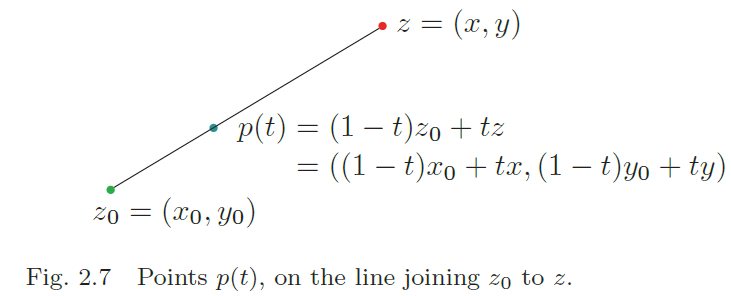
\includegraphics[width=0.6\textwidth]{./SaltChapter/fig-2-7}
\end{center}
\caption{$z_0$와 $z$를 잇는 직선 위의 점 $p(t)$}
\label{fig-2-7}
\end{figure}











%===[salt] 3장
% !TEX root = ../notes_template.tex

\chapter{코시 적분 정리와 응용}

복소미분은 어느정도 익숙해졌으니 이제 적분으로 관심을 돌려보자.
이 장에서는 복소해석학에서 매우 중요한 다음 정리를 배울 예정이다.
\begin{center}
\fbox{
코시 적분 정리
}
\end{center}
``경로적분''을 정의하는 것으로 시작하여 나중에 코시 적분 정리를 증명할 예정이다.
왜 경로적분과 코시 적분 정리가 왜 그렇게 중요한지 의문을 가질 수 있다.
복소평면에서 적분의 중요성은 복소해석함수의 더 큰 이해로 이어지기 때문이다.
예를 들면, 복소해석함수는 무한번 미분가능하다는 본질적인 성질이 있다.
이 장에서 다음 주제들을 중심으로 공부해보기로 하자.
\begin{enumerate}
\item[(1)] 경로적분의 정의와 성질
\item[(2)] 경로적분의 기본정리
\item[(3)] 코시 적분 정리
\item[(4)] 코시 적분 정리의 응용
\begin{enumerate}
\item 부정적분의 존재성
\item 복소해석함수의 무한번 미분가능성
\item 리우비우 정리와 대수학의 기본정리
\item 모레라 정리
\end{enumerate}
\end{enumerate}

\section{경로적분의 정의}

일반적인 미적분에서 연속함수 $f: [a,b] \to \mathbb R$가 주어질 때
\begin{equation}\label{eq-3-1}
\int_a^b f(x)dx
\end{equation}
의 의미는 명확하다. 이제 이를  일반화하여 복소수까지 확장하고
주어진 복소수 $z$, $w$에 대하여
\[
\int_z^w f(\zeta)d\zeta
\]
에 의미를 부여하길 원한다고 하자.
$z$에서 $w$까지를 어떻게 해석해야 할까?

$\mathbb R$에서 $a<b$이면, 실수 $a$부터  실수 $b$까지
가는 경로는 한가지 뿐이다.  
따라서 실수의 경우는 단지
\begin{itemize}
\item[(1)] $a<b$이고,
\item[(2)] 연속함수 $f:[a,b] \to \mathbb R$
\end{itemize}
의 경우만 생각하면 충분하다.

하지만, $z$와 $w$가 복소평면 위의 점이면
그림 \ref{fig-3-1}과 같이 많은 경로에 대하여 적분을 생각할 수 있다.

\begin{figure}[!h]
\begin{center}
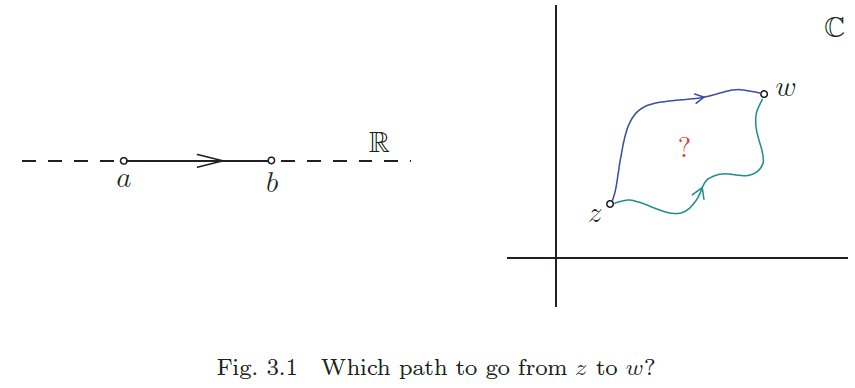
\includegraphics[width=0.8\textwidth]{./SaltChapter/fig-3-1}
\end{center}
\caption{$z$에서 $w$까지 어떤 경로로 가야할까?}
\label{fig-3-1}
\end{figure}

그러므로 복소수의 경우는 끝점 $z$와 $w$ 외에
$z$에서 $w$까지의 경로 $\gamma$도 지정하고,
실수의 경우를 나타낸 식 \eqref{eq-3-1}를
다음과 같이 복소수에 대한 표현으로 바꾸도록 한다.
\[
\int_\gamma f(z)dz.
\]

이 표현을 ``경로''적분이라 부르며
계산을 위해 다음을 정할 필요가 있다.
\begin{itemize}
\item[(1)] 정의역  $D(\subset \mathbb C)$와 $z, w\in D$
\item[(2)] 연속함수 $f:D\to \mathbb C$
\item[(3)] $z$와 $w$를 잇는 매끄러운 경로 $\gamma: [a,b] \to D$
\end{itemize}



%===[salt] 4장
% !TEX root = ../notes_template.tex

\chapter{테일러 급수와 로랑 급수}

이 장에서는 영역 $D$에 정의된 복소해석함수 $f$는 
$D$의 임의의 점에서 급수 전개가 가능하다는 근본적인 성질을 먼저 공부할 것이다.
다음 그림에서 왼쪽을 참고하라.
\begin{figure*}[h!]
\begin{center}
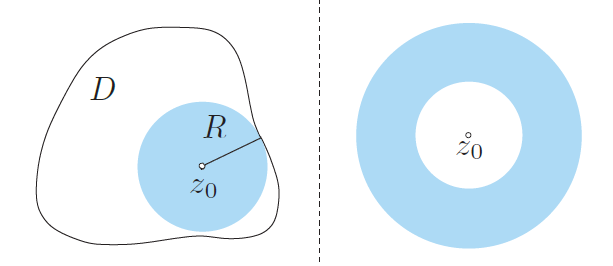
\includegraphics[width=0.5\textwidth]{./SaltChapter/fig-4-0-1}
\end{center}
\end{figure*}
\[
\text{테일러 급수: } \sum_{n=0}^\infty c_n(z-z_0)^n 
\quad
\text{로랑 급수: } \sum_{n\in \mathbb Z} c_n(z-z_0)^n 
\]

즉, 각각의 $z_0 \in D$에 대하여 다음을 만족하는 $R>0$이 존재한다.
\[
f(z) = \sum_{n=0}^\infty c_n(z-z_0)^n, \quad |z-z_0| <R.
\]
역으로,  적당한 $R$에 대하여 $|z-z_0|<R$을 만족하는 두 개 이상의 점에서 급수
\[
\sum_{n=0}^\infty c_n(z-z_0)^n
\]
가 수렴하면 $|z-z_0|<R$에서 복소해석함수이다.
이를 보이는 과정에서 복소해석함수에 대한 근본적인 성질들을 증명할 것이다.
\begin{itemize}
\item[(1)] (일반화된) 코시 적분공식과 코시 부등식
\item[(2)] 해의 분류와 항등정리
\item[(3)] 최대절대값정리
\end{itemize}

이 장의 후반부에서는
급수와 유사하지만 $z-z_0$ 항의 지수를 음의 정수까지 확장한
로랑 급수를 공부할 것이다.
이는 원환(특히 뚫린 원판)에 정의된 복소해석함수를 연구하는데 특히 유용하다,
앞의 그림에서 오른쪽을 참고하라.
끝으로 로랑 급수는 ``특이점''의 분류와 실함수 적분의 계산에도 유용함을 살펴볼 것이다.

\section{급수}

실수열의 경우와 유사하게 주어진
복소수열 $(a_n)_{n\in\mathbb N}$에 대하여
부분합 수열 $(s_n)_{n\in\mathbb N}$을 만들 수 있다.
\begin{align*}
s_1 &:= a_1, \\
s_2 &:= a_1 + a_2, \\
s_3 &:= a_1 + a_2 + a_3, \\
& \vdots
\end{align*}

\begin{salt_definition} \label{def-4-1}
\
\begin{itemize}
\item[(1)] 복소수열 $(s_n)_{n\in\mathbb N}$이 수렴하면
$\sum\limits_{n=1}^\infty a_n := \lim\limits_{n\to\infty} s_n$라 쓰고
급수 $\sum\limits_{n=1}^\infty a_n$이 {\bf 수렴한다}고 정의한다.
\item[(2)] 복소수열 $(s_n)_{n\in\mathbb N}$이 발산하면,
급수 $\sum\limits_{n=1}^\infty a_n$는 {\bf 발산한다}고 정의한다.
\item[(3)] 실급수 $\sum\limits_{n=1}^\infty |a_n|$이 수렴하면,
급수 $\sum\limits_{n=1}^\infty a_n$은 {\bf 절대수렴한다}고 정의한다.
\end{itemize}
\end{salt_definition}

복소수열이 수렴할 필요충분조건은
실수부와 허수부로 만든 수열이 각각 수렴하는 것이라는 
연습문제 \ref{ex-1-25}의 결과로부터,
\[
\sum\limits_{n=1}^\infty a_n\,\text{이 수렴한다. }
\Longleftrightarrow \text{\textcolor{red}{ 실수열} }
\sum\limits_{n=1}^\infty \Re(a_n)\, \text{과 }
\sum\limits_{n=1}^\infty \Im(a_n)\,\text{가 수렴한다.}
\]
따라서  실해석학의 결과를 아용하여 복소수열의 수렴성을 판정할 수 있다.
예를 들면, 다음 결과들을 쉽게 얻을 수 있는데 이는 연습문제로 남긴다.

\begin{salt_exercise}\label{ex-4-1}
$\Sum_{n=1}^\infty a_n$이 수렴하면, $\Lim_{n\to\infty}a_n = 0$임을 보여라.
\end{salt_exercise}

\begin{salt_exercise}\label{ex-4-2}
$\Sum_{n=1}^\infty a_n$이 절대수렴하면, $\Sum_{n=1}^\infty a_n$이 수렴함을 증명하라.
\end{salt_exercise}

\begin{salt_exercise}\label{ex-4-3}
$|z|<1$이면 $\Sum_{n=0}^\infty z^n$이 수렴하고 
$\Sum_{n=0}^\infty z^n = \dfrac1{1-z}$임을 보여라.
\end{salt_exercise}

\begin{salt_exercise}\label{ex-4-4}
$|z|<1$이면 $\Sum_{n=0}^\infty nz^{(n-1)^2}$임을 보여라.
\end{salt_exercise}

\begin{salt_exercise}\label{ex-4-5}
$\Re(s)>0$인 모든 복소수 $s\in \mathbb C$에 대하여
$1^{-s} +  2^{-s} + 3^{-s} + \cdots$가 수렴함을 보여라.
그러면
\[
s \mapsto \zeta(s) := \sum_{n=1}^\infty \dfrac1{n^s}
\]
\end{salt_exercise}
는 반평면 $\Re(s)>1$에서 잘 정의된 함수가 되며, 이를 
{\bf 리만 제타함수}라고 한다.
리만 제타함수와 정수론의 소수이론을 연결한 {\bf 오일러 곱셈공식}에 따르면,
소수를 증가하는 순서대로 나열한
$p_1:=2 < p_2:=3 < p_3:=5 < \cdots$를 무한 소수열로 정의할 때 다음이 성립한다.
\[
\zeta(s) = \lim_{K\to \infty} \prod_{k=1}^K \dfrac1{1-p_k^{-s}},
\quad \Re(s)>1.
\]
버나드 리만(1826-1866)은 제타함수 $\zeta$를 확장하여 $\mathbb C\setminus \{1\}$의 
복소해석함수로 정의할 수 있음을 보였다. 
$\zeta$는 $-2, -4, -6, \ldots$에서 ``자명해(trivial zero)''를 갖지면
다른 해도 존재한다. 리만이 계산한 모든 비자명해(nontrivial zero)는 모두 직선 $\Re(s) = 1/2$위에
있다. 이로부터 리만은 다음과 같이 예측(conjecture)하였는데 이는 여전히 수학계의 유명한 미해결 문제이다.

\begin{salt_conjecture}[리만가설] \label{conj-4-1}
리만 제타함수의 모든 비자명해는 직선 $\Re(s) = 1/2$ 위에 있다.
\end{salt_conjecture}

\section{급수}

\subsection{제곱급수와 수렴영역}

$(c_n)_{n\in\mathbb N}$을 복소수열이라고 하자.
다음과 같은 표현을
\[
\sum_{n=0}^\infty c_nz^n
\]
복소수 변수 $z$의 제곱급수라고 한다 ($(c_n)_{n\in\mathbb N}$을 계수들의 수열로 생각해도 된다).
이제 특정한 값을 급수의  $z$에 대입하는 경우를 생각해볼 수 있다.
그러면 어떤 $z\in\mathbb C$에 대하여 제곱급수가 수렴할 수 있고, 
다른 값에서는 발산할 수도 있다.

\begin{salt_example}\label{example-4-1}
모든 다항식은 유한개의 항에서만 계수가 $0$이 아닌 제곱급수 꼴로 쓸 수 있다.
따라서 다항식은 모든 $z\in\mathbb C$에 대하여 수렴한다.

제곱급수  
\[
\sum_{n=0}^\infty z^n
\]
는 $|z|<1$에서 수렴한다. 
$|z|\ge1$에서 급수는 발산한다 (왜냐하면 $\Lim_{n\to\infty} z^n = 0$이 성립하지 않으므로).
\hfill$\diamondsuit$
\end{salt_example}

근본적인 질문으로 
\begin{center}
어떤 $z\in\mathbb C$에 대하여  급수 $\sum_{n=0}^\infty c_nz^n$가 수렴하는가?
\end{center}

이 문제에 대한 답은 다음 정리에서 얻을 수 있다.

\begin{salt_theorem} \label{thm-4-1}
제곱급수 $\Sum_{n=0}^\infty c_nz^n$에 대하여
다음 두 가지 중 정확히 하나만 성립한다.
\begin{itemize}
\item[(1)] 모든 $z\in\mathbb C$에 대하여 절대수렴하거나
\item[(2)] 음이 아닌 실수 $R$이 유일하게 존재하여 다음을 만족한다.
\begin{itemize}
\item[(a)] $|z|<R$인 모든 $z\in\mathbb C$에 대하여 $\Sum_{n=0}^\infty c_nz^n$이 절대수렴하고,
\item[(b)] $|z|>R$인 모든 $z\in\mathbb C$에 대하여 $\Sum_{n=0}^\infty c_nz^n$는 발산한다.
\end{itemize}
\end{itemize}
\end{salt_theorem}

위 정리에서 유일한 $R>0$을 급수의 수렴반경이라 부른다.
급수가 모든 $z\in\mathbb C$에 대하여 수렴하면
무한대의 수렴반경을 가지며 ``$R=\infty$''라 쓴다.

\begin{figure}[h!]
\begin{center}
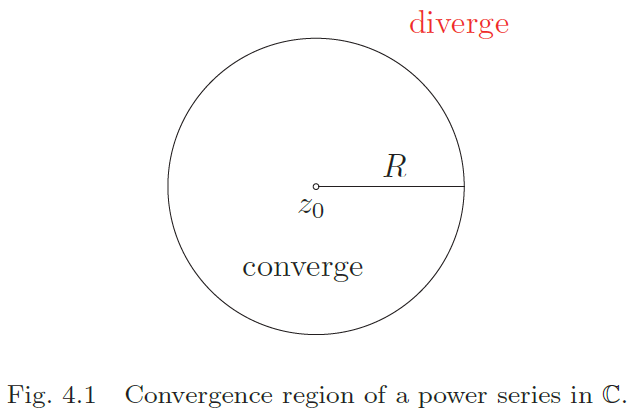
\includegraphics[width=0.5\textwidth]{./SaltChapter/fig-4-1}
\end{center}
\caption{$\mathbb C$에 정의된 제곱급수의 수렴영역}
\label{fig-4-1}
\end{figure}

원 $|z|=R$에서는 어떻게 될까?
복소 제곱급수는 $|z|=R$로 주어진 경계의 모든 점에서 발산하거나,
어떤 점에서는 발산하고 어떤 점에서는 수렴하거나,
아니면 경계의 모든 점에서 수렴할 수도 있다.
경계위의 각 점에 대하여 어떻게 되는지 답을 구하는 일반적인 방법은 없다.
특정한 제곱급수가 주어지면 그 특성에 따라 찾아 직접 확인해야 한다,

{\bf 증명} (정리 \ref{thm-4-1})

\[
S:= \left\{ y\in [0,\infty) \,:\,
\exists z\in \mathbb C, y=|z| \text{ 이고 } \Sum_{n=0}^\infty c_nz^n \text{이 수렴한다.}
\right\}
\]
라 정의하자.
$0\in S$은 분명하기에 $S$는 공집합이 아니며
다음 두 가지 경우가 가능하다.

$\underline{1}^\circ$ $S$가 위로 유계가 아닌 경우:
이 경우는 수렴반경은 무한대가 됨을 보일 것이다.
$z\in \mathbb C$가 주어졌다고 하면,
$|z|<y$인 $y\in S$가 존재한다.
 그런데 $y\in S$이므로 $y=|z_0|$이고
\[
\sum_{n=0}^\infty c_n z_0^n
\]
이 수렴하는 $z_0\in S$가 존재한다.
이로부터 $n\to\infty$일 때 각 항이 $0$으로 수렴한다.
특히, 각 항은  $|c_nz_0^n| \le M$으로 유계이다.
이제 $r:=|z|/|z_0| (<1)$로 잡으면
\[
|c_nz^n| = |c_nz_0^n| \left( \dfrac{|z|}{|z_0|}\right)^n
\le Mr^n \quad (n\in \mathbb N).
\]
한편 $\sum\limits_{n=0}^\infty Mr^n$이 수렴한다 ($r<1$).
비교판정법을 쓰면 
\[
\sum_{n=0}^\infty c_n z^n
\]
은 절대수렴한다. $z$는 우리가 임의로 선택할 수 있기 때문에
정리의 (1)이 성립한다,


$\underline{2}^\circ$ $S$가 위로 유계인 경우:
이 경우 수렴반경이 $\sup S$가 됨을 보일 것이다.
즉,
\begin{itemize}
\item[(a)] $|z|<\sup S$이면
$\Sum_{n=0}^\infty c_nz^n$이 절대수렴하고,
\item[(b)] $|z|>\sup S$이면  $\Sum_{n=0}^\infty c_nz^n$는 발산한다.
\end{itemize}
$z\in S$가 $|z|<\sup S$를 만족하면
상계(supremum)의 %= ##[SALT] 용어확인
정의에 따라,
$|z|<y$인 $y\in S$가 존재한다. 
그러면 $\underline{1}^\circ$ $S$의 증명과정을 아래와 같이 반복할 수 있다.
$y\in S$이므로
$y=|z_0|$이고
\[
\sum_{n=0}^\infty c_n z_0^n
\]
이 수렴하는 $z_0\in S$가 존재한다.
이로부터 $n\to\infty$일 때 각 항이 $0$으로 수렴한다.
특히, 각 항은 $|c_nz_0^n| \le M$으로 유계이다.
이제 $r:=|z|/|z_0| (<1)$로 잡으면
\[
|c_nz^n| = |c_nz_0^n| \left( \dfrac{|z|}{|z_0|}\right)^n
\le Mr^n \quad (n\in \mathbb N).
\]
한편 $\sum\limits_{n=0}^\infty Mr^n$이 수렴한다 ($r<1$).
비교판정법을 쓰면 
\[
\sum_{n=0}^\infty c_n z^n
\]
은 절대수렴한다.
끝으로, $z\in \mathbb C$가 $|z|>\sup S$를 만족하면,
$y:=|z|$라 할 때
$y \in S$이고 $S$의 정의로부터 
\[
\sum_{n=0}^\infty c_n z^n
\]
이 발산한다 (그렇지 않다면 $y\in S$를 만족해야 한다).

\begin{figure*}[h!]
\begin{center}
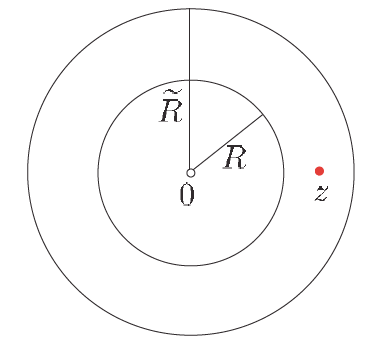
\includegraphics[width=0.3\textwidth]{./SaltChapter/fig-4-0-2}
\end{center}
%\caption{$\mathbb C$에 정의된 제곱급수의 수렴영역}
%\label{fig-4-1}
\end{figure*}

$R$의 유일성은 다음과 같이 증명된다.
$R$과 $\tilde R$이 정리의 조건을 만족하고 $R<\tilde R$이라 하자.
그러면
\[
R < r:= \dfrac{R+\tilde R}{2} < \tilde R.
\]
$r<\tilde R$로부터
$\Sum_{n=0}^\infty c_n r^n$이 수렴하고,
$R<r$로부터 $\Sum_{n=0}^\infty c_n r^n$은 발산하며
모순이 된다.
\hfill $\square$

다음 결과를 이용하면
몇가지 경우의 수렴반경를 계산할 수 있다,

 \begin{salt_theorem} \label{thm-4-2}
제곱급수 
\[
\Sum_{n=0}^\infty c_nz^n
\]에 대하여 극한
$L:= \Lim_{n\to\infty} \left| \dfrac{c_{n+1}}{c_n}\right|$가
존재한다고 하자. 
\begin{itemize}
\item[(1)] $L\ne0$이면, 수렴반경은 $1/L$이고,
\item[(2)] $L=0$이면, 수렴반경은 무한대이다.
\end{itemize}
\end{salt_theorem}

{\bf 증명}

$L\ne0$이라 하자.
그러면 $|z|<1/L$인 모든 $z\ne0$에 대하여
$q<1$와 충분히 큰 $N$이 존재하여
\[
\dfrac{|c_{n+1}z^{n+1}|}{|c_nz^n|}
= \left| \dfrac{c_{n+1}}{c_n}\right| |z| \le q <1
\quad (n>N)
\]
을 만족한다
(왜냐하면,
\[
\left|\dfrac{c_{n+1}}{c_n}z\right|
\stackrel{n\to\infty}{\longrightarrow}
L|z|<1
\]
이므로 $q=(L|z|+1)/2 <1$로 잡으면 된다).
비율판정법을 적용하면 급수는 절대수렴한다.

$L=0$이면 $0$이 아닌 모든 $z\in \mathbb C$에 대하여
$q<1$가 존재하여
\[
\dfrac{|c_{n+1}z^{n+1}|}{|c_nz^n|}
= \left| \dfrac{c_{n+1}}{c_n}\right| |z| \le q <1
\quad (n>N)
\]
을 만족한다 (왜냐하면
\[
\left|\dfrac{c_{n+1}}{c_n}z\right|
\stackrel{n\to\infty}{\longrightarrow}
0|z|=0<1
\]
이므로 $q=1/2<1$도 두면된다).
따라서 비율판정법을 다시 쓰면 급수는 절대수렴한다.

한편, $L\ne0$이고 $|z|>1/L$이면,
$\left|\dfrac{c_{n+1}z}{c_n}\right|
\stackrel{n\to\infty}{\longrightarrow}
L|z|>1$이므로
충분히 큰 $N$이 존재하여
\[
\dfrac{|c_{n+1}z^{n+1}|}{|c_nz^n|}
= \left| \dfrac{c_{n+1}}{c_n}\right| |z|>1
\quad (n>N)
\]
을 만족한다.
이 경우 비율판정법에 따라 급수는 발산한다.
\hfill $\square$

\begin{salt_example}\label{example-4-2}
\[
\lim_{n\to\infty} \dfrac{\dfrac1{(n+1)^2}}{\dfrac1{n^2}} = 1
\]
이므로 
급수 $\Sum_{n=1}^\infty \dfrac{z^n}{n^2}$는
$|z|<1$에서 수렴하고
$|z|>1$에서 발산한다.
$|z|=1$이면
\[
\left| \dfrac{z^n}{n^2} \right| = \dfrac1{n^2}
\]
이므로 급수 $\Sum_{n=1}^\infty \dfrac{1}{n^2}$는
절대수렴한다. 즉, 원 $|z|=1$ 위의 모든 점에서 급수가 수렴한다.
한편 기하급수 
\[
\sum_{n=0}^\infty z^n
\]
은 원 $|z|=1$ 위의 어떤 점에서도 수렴하지 않는다.
\hfill$\diamondsuit$
\end{salt_example}

\begin{salt_exercise}\label{ex-4-6}
급수 $\Sum_{n=0}^\infty c_nz^n$에 대하여
극한 $L:=\Lim_{n\to\infty} sqrt[n]{|c_n|}$이 존재할 때
다음을 보여라.
\begin{itemize}
\item[(1)] $L\ne 0$이면 수렴반경은 $1/L$이다.
\item[(2)] $L\ne0$이면 수렴반경은 무한대이다.
\end{itemize}
\end{salt_exercise}

\begin{salt_exercise}\label{ex-4-7}
급수 $\Sum_{n=1}^\infty n^nz^n$은
$z=0$에서만 수렴함을 보여라.
\end{salt_exercise}

\begin{salt_exercise}\label{ex-4-8}
급수 $\Sum_{n=1}^\infty \dfrac{z^n}{n^n}$은
모든 $z\in\mathbb C$에 대하여 수렴함을 보여라.
\end{salt_exercise}

\begin{salt_exercise}\label{ex-4-9}
다음 복소제곱급수의 수렴반경을 구하라.
\[
\sum_{n=1}^\infty \dfrac{(-1)^n}{n}z^n,\quad
\sum_{n=0}^\infty n^{2012}z^n, \quad
\sum_{n=0}^\infty \dfrac1{n!}z^n.
\]
\end{salt_exercise}

\subsection{복소해석함수의 제곱급수}

다항식은 수렴반경이 무한대인 제곱급수로 간주할 수 있다.
즉, 모든 $\mathbb C$에서 수렴한다.
이 성질은 복소해석함수에서도 성립하는데
이는 우연이 아니다.
일반적으로 제곱급수 
\[
f(z):= \sum_{n=0}^\infty c_nz^n
\]
가 $|z|<R$에 대하여 수렴하면
$|z|<R$에서 복소해석함수가 되며 
다음 등식이 성립한다.
\[
f'(z) = \dfrac d{dz} (c_0+ c_1z + c_2z^2 + \cdots)
= c_1 + 2c_2z + 3c_3z^3 + \cdots 
= \sum_{n=1}^\infty c_n n z^{n-1}.
\]
(항의 개수가 유한한 경우, 즉, 다항식처럼 
항별 미분이 가능할 것으로 예상한 결과와 같다)

\begin{salt_theorem}\label{thm-4-3}
$R>0$이고 $f(z):= \Sum_{n=0}^\infty c_nz^n$가
$|z|<R$에서 수렴한다고 하면
$f'(z) = \Sum_{n=1}^\infty c_n n z^{n-1}$.
\end{salt_theorem}

{\bf 증명}

{\bf 단계 1.}
우선 다음 제곱급수가 $|z|<R$에서 절대수렴함을 보이자.
\[
g(z):= \Sum_{n=1}^\infty c_n n z^{n-1}
=  c_1 + 2c_2z + 3c_3z^3 + \cdots
\]
$z$는 고정하자.
$|z|<r<R$을 만족하는 $r$을 잡으면, 가정으로부터
\[
\Sum_{n=0}^\infty c_nr^n
\]
이 수렴한다. 따라서 모든 $n$에 대하여
$|c_nr^n|<M$을 만족하는 양수 $M$이 존재한다.
$\rho:=|z|/r$이라 하면, $0\le \rho <1$이고,
\[
|nc_nz^{n-1}| = |c_nr^n| \cdot 
\dfrac1r \cdot n \left| \dfrac zr\right|^{n-1}
\le \dfrac{Mn\rho{n-1}}r.
\]
$\Sum_{n=1}^\infty n\rho^{n-1}$은 
($1/(1-\rho)^2$으로) 수렴한다 (연습문제 \ref{ex-4-4} 참고).
따라서 비교판정법에 의해
$\Sum_{n=1}^\infty nc_nz^{n-1}$은 절대수렴한다.

{\bf 단계 2.}
이제 $|z_0|<R$에 대하여 $f'(z_0) = g(z_0)$임을 보이자. 즉,
\[
\lim_{z\to z_0} \left(
\dfrac{f(z)-f(z_0)}{z-z_0} - g(z_0) \right) = 0.
\]
단계 1에서 했던 것처럼 $|z_0|<r<R$을 만족하는 $r$을 잡으면, 
$z\to z_0$로부터 $|z|<r$도 성립한다.

\begin{figure*}[h!]
\begin{center}
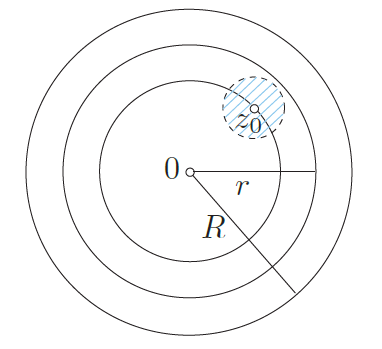
\includegraphics[width=0.3\textwidth]{./SaltChapter/fig-4-0-3}
\end{center}
%\caption{$\mathbb C$에 정의된 제곱급수의 수렴영역}
%\label{fig-4-0-3}
\end{figure*}

$\epsilon>0$이라 하자.
$\Sum_{n=1}^\infty nc_nr^{n-1}$이 절대수렴하므로
다음을 만족하는 $N$이 존재한다.
\[
\Sum_{n=N}^\infty \left| nc_nr^{n-1}\right| < \dfrac \epsilon4.
\]
이제부터 $N$을 고정하자.
$f(z) - f(z_0) = \Sum_{n=1}^\infty c_n(z^n - z_0^n)$이므로,
$z\ne z_0$에 대하여
\[
\dfrac{f(z)-f(z_0)}{z-z_0}  
= \sum_{n=1}^\infty c_n \dfrac{z^n-z_0^n}{z-z_0}
= \sum_{n=1}^\infty c_n \left(
z^{n-1} + z^{n-2}z_0 + \cdots + z_0^{n-1} \right).
\]
따라서,
\[
\dfrac{f(z)-f(z_0)}{z-z_0}   - g(z_0)
= \sum_{n=1}^\infty c_n \dfrac{z^n-z_0^n}{z-z_0}
= \sum_{n=1}^\infty c_n \left(
z^{n-1} + z^{n-2}z_0 + \cdots + z_0^{n-1} - nz_0^{n-1}\right).
\]
이 급수에서 처음 $N-1$개 항의 합을 $S_1$이라 하고
(즉, $n=1$에서 $n=N-1$까지),
$S_2$를 나머지 항의 합이라고 하자.
그러면, $|z|, |z_0| < r$로부터
\[
|S_2| \le \sum_{n=N}^\infty |c_n| 
\left( \underbrace{r^{n-1}+r^{n-1} + \cdots + r^{n-1}}_{n\text{개 항}}
+ nr^{n-1}\right)
= \sum_{n=N}^\infty 2n|c_n|r^{n-1} < \dfrac\epsilon2.
\]
한편,
\[
S_1= \sum_{n=1}^N c_n \left(
z^{n-1} + z^{n-2}z_0 + \cdots + zz_0^{n-2} + z_0^{n-1} - nz_0^{n-1}
\right)
\]
는 $z$의 다항식이며 극한은 다음과 같다.
\begin{align*}
\lim_{z\to z_0} S_1
&= \sum_{n=1}^N c_n \left(
z^{n-1} + z^{n-2}z_0 + \cdots + zz_0^{n-2} + z_0^{n-1} - nz_0^{n-1}
\right) \\
&= \sum_{n=1}^N c_n \left(
nz_0^{n-1}  - nz_0^{n-1} \right) = 0.
\end{align*}
따라서
$|z-z_0|<\delta$이면, $|S_1|< \epsilon/2$가 되는 
양수 $\delta$가 존재한다.
이제 $|z|<r$이고 $0<|z-z_0|< \delta$에 대하여
\[
\left| \dfrac{f(z)-f(z_0)}{z-z_0}   - g(z_0) \right|
\le |S_1| + |S_2| <  \dfrac\epsilon2 + \dfrac\epsilon2 = \epsilon.
\]
이로써 $f'(z_0) = g(z_0)$가 증명된다.
\hfill $\square$

\begin{salt_remark} \label{rem-4-1}
$(c_n)_{n\in\mathbb N}$이 실수열일 때,
실제곱급수
\[
\sum_{n=0}^\infty c_nx^n
\]
\end{salt_remark}
를 생각해보자. 실해석의 결과로부터 어떤 $R>0$이 존재하여
이 제곱급수는 구간 $(-R, R)$에서 수렴하고
$\mathbb R \setminus [-R,R]$에서 발산한다.
정리 \ref{thm-4-1}과 \ref{thm-4-3}로부터
실변수 $x$를 복소변수 $z$로 바꾸면 실제곱급수의 결과가 
복소평면의 원판 $|z|<R$에 정의된 복소해석함수로 확장됨을 알 수 있다.
따라서
실해석함수(즉, 국소적으로 제곱급수 전개를 갖는 실변수함수)는
복소해석함수를 실수축에 제한한 것으로 볼 수 있다.
이 결과로 실해석학과 복소해석학의 세계를 연결하는
상호작용을 엿볼 수 있다
(우리는 코시-리만 방정식을 공부하면서 이미 이러한 사례를 살펴 본 바 있다).

앞의 결과를 반복하면 다음을 쉽게 얻는다.

\begin{salt_corollary}\label{coro-4-1}
$R>0$이고, $f(z):= \Sum_{n=0}^\infty c_n z^n$이 $|z|<R$에서 수렴한다고 하자.
그러면, $k\ge1$에 대하여
\begin{equation}\label{eq-4-1}
f^{(k)}(z) = \sum_{n=k}^\infty n(n-1)(n-2)\cdots (n-k+1)c_nz^{n-k}.
\quad (|z|<R)
\end{equation}
특히, $n\ge0$에 대하여, $c_n = \dfrac1{n!} f^{(n)}(0)$.
\end{salt_corollary}

{\bf 증명}

직접 계산하여 바로 얻을 수 있는 결과이며, 두번째 결과를 얻기 위해
식 \eqref{eq-4-1}에 $z=0$을 대입하면
\[
f^{(k)}(0) = k(k-1)\cdots 1c_k + z \sum{n=k+1}^\infty n(n-1) \cdots (n-k+1)c_n z^{n-k-1}\Big|_{z=0}
= k!c_k
\]
이며, $f(0)=c_0$이다.
\hfill $\square$

이는 $0$을 중심으로 전개한 제곱급수에 한정된 결과가 아니다.
복소수 $z_0$를 택하여 제곱급수
\[
\sum_{n=0}^\infty c_n(z-z_0)^n
\]
를 생각하면, 정리 \ref{thm-4-1}과 \ref{thm-4-3}으로부터
다음 결과를 바로 얻는다.


\begin{salt_corollary} \label{thm-4-2}
제곱급수 $\Sum_{n=0}^\infty c_n(z-z_0)^n$에 대하여
다음 두 가지 중 정확히 하나만 성립한다.
\begin{itemize}
\item[(1)] 모든 $z\in\mathbb C$에 대하여 절대수렴하거나
\item[(2)] 음이 아닌 실수 $R$이 유일하게 존재하여 다음을 만족한다.
\begin{itemize}
\item[(a)] $|z-z_0|<R$인 모든 $z\in\mathbb C$에 대하여 
$\Sum_{n=0}^\infty c_n(z-z_0)^n$이 절대수렴하고,
\item[(b)] $|z-z_0|>R$인 모든 $z\in\mathbb C$에 대하여 
$\Sum_{n=0}^\infty c_n(z-z_0)^n$는 발산한다.
\end{itemize}
\end{itemize}
\end{salt_corollary}

\begin{salt_corollary}\label{coro-4-3}
$z_0\in \mathbb C$, $R>0$이고, 
$f(z):= \Sum_{n=0}^\infty c_n (z-z_0)^n$이 $|z-z_0|<R$에서 수렴한다고 하자.
그러면, $k\ge1$에 대하여
\begin{equation}\label{eq-4-1}
f^{(k)}(z) = \sum_{n=k}^\infty n(n-1)(n-2)\cdots (n-k+1)c_n(z-z_0)^{n-k}.
\quad (|z-z_0|<R)
\end{equation}
특히, $n\ge0$에 대하여, $c_n = \dfrac1{n!} f^{(n)}(z_0)$.
\end{salt_corollary}

\begin{salt_remark} [계수의 유일성] \label{rem-4-2}
중심이 $z_0$, 반지름 $R>0$인 열린원판에서
두 제곱급수
\[
\Sum_{n=0}^\infty c_n(z-z_0)^n \quad\text{와}\quad
\Sum_{n=0}^\infty \tilde c_n(z-z_0)^n
\]
가 모두 같은 함수 $f$로 수렴한다고 하자.
그러면 위의 따름정리로부터 모든 $n\ge0$에 대하여
\[
c_n = \dfrac{f^{(n)}(z_0)}{n!} = \tilde c_n.
\]
\end{salt_remark}

\begin{salt_exercise} \label{ex-4-10}
$|z|<1$일 때,
$1^2 + 2^2z + 3^2z^2 + 4^2z^3 + \cdots$의 값은?
\end{salt_exercise}

\begin{salt_exercise} \label{ex-4-11}
제곱급수 $\Sum_{n=0}^\infty c_nz^n$에 대하여 다음 문장의 참, 거짓을 판정하라.
\begin{itemize}
\item[(1)] 급수가 수렴하는  복소수 $z$의 집합은 $\{0\}$이거나, 유한한 반지름을 갖는 열린원판,
또는 복소평면 전체가 되며 다른 경우는 생길 수 없다.
\item[(2)] 제곱급수가 $z=1$에서 수렴하면 $|z|<1$에서 수렴한다.
\item[(3)] 제곱급수가 $z=1$에서 수렴하면 원 $|z|=1$의 모든 점에서 수렴한다.
\item[(4)] 제곱급수가 $z=1$에서 수렴하면 $z=-1$에서 수렴한다.
\item[(5)] 제곱급수가 원점이 중심이고 반지름이 유한한 열린원판에서 수렴하면
원판의 경계(즉, 원판을 둘러싸는 원)의 전체 또는 일부에서도 수렴할 수 있으나
그 이외의 점에서는 수렴할 수 없다.
\item[(6)] 수렴하는 범위가 닫힌원판 $|z|\le 1$ 전체인 제곱급수가 존재한다.
\item[(7)] 제곱급수가 $z=i$에서 발산하면, $z=1+i$에서도 발산한다.
\end{itemize}
\end{salt_exercise}

\section{테일러 급수} \label{section-4-3}

앞 절에서 수렴반경이 $R$인 복수제곱급수
\[
\sum_{n=0}^\infty c_n(z-z_0)^n
\]
은 영역 $|z-z_0|<R$에서 복소해석함수가 됨을 살펴보았다.
이 절에서는 역으로 $f$가 원판 $|z-z_0|<R$에서 복소해석함수이면
\[
f(z) = \sum_{n=0}^\infty c_n (z-z_0)^n \quad (|z-z_0|<R)
\]
임을 보일 것이다. 여기서 계수 $c_n$은 $f$로부터 결정된다.
따라서 영역 $D$에 정의된 복소해석함수 $f$는 임의의 점 $z_0\in D$의 근방에서
제곱급수 전개를 갖는다.

\begin{salt_theorem}\label{thm-4-4}
$f$가 $D(z_0,R) := \{ z\in \mathbb C \,:\, |z-z_0| <R \}$에서 복소해석함수이면,
$z\in D(z_0,R)$에 대하여
$f(z) = c_0 + c_1(z-z_0) + c_2(z-z_0)^2 + c_3(z-z_0)^3+ \cdots$이다.
여기서, $n\ge0$에 대하여
\[
c_n = \dfrac1{2\pi i} \int_C \dfrac{f(\zeta)}{(\zeta-z_0)^{n+1}} d\zeta
\]
이고, $C$는 중심이 $z_0$이고 반지름 $r$ ($0<r<R$)인 원을 반시계방향으로 도는 원이다.
\end{salt_theorem}

\begin{figure*}[h!]
\begin{center}
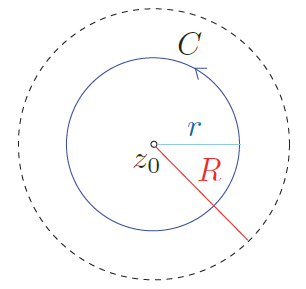
\includegraphics[width=0.3\textwidth]{./SaltChapter/fig-4-0-4}
\end{center}
%\caption{$\mathbb C$에 정의된 제곱급수의 수렴영역}
%\label{fig-4-0-3}
\end{figure*}

{\bf 증명}

$z\in D(z_0, R)$이라 하자.
우선 $|z-z_0|<r<R$인 $r$을 잡고
코시 적분공식을 적용하면
\begin{align*}
f(z) &= \dfrac1{2\pi i}\int_C \dfrac{f(\zeta)}{\zeta-z} d\zeta
= \dfrac1{2\pi i}\int_C \dfrac{f(\zeta)}{\zeta-z_0+z_0-z} d\zeta \\
&= \dfrac1{2\pi i}\int_C \dfrac{f(\zeta)}{(\zeta-z_0)\left(1- \dfrac{z-z_0}{\zeta-z_0}\right)} d\zeta.
\end{align*}
$w:=\dfrac{z-z_0}{\zeta-z_0}$라 하면,
$|w| = \dfrac{|z-z_0|}r <1$이므로
\begin{align*}
\dfrac1{1-\dfrac{z-z_0}{\zeta-z_0}} = \dfrac1{1-w}
& = 1+ w + w^2 + w^3 + \cdots + w^{n-1} + \dfrac{w^n}{1-w} \\
&= 1 + \dfrac{z-z_0}{\zeta-z_0} + \cdots + \dfrac{(z-z_0)^{n-1}}{(\zeta-z_0)^{n-1}}
+ \dfrac{(z-z_0)^n}{(\zeta-z_0)^{n-1}(\zeta-z)}.
\end{align*}
이 결과를 종합하면
\begin{align*}
f(z) &= \dfrac1{2\pi i}\int_C f(\zeta) \left(
\dfrac1{\zeta-z_0} + \cdots + \dfrac{(z-z_0)^{n-1}}{(\zeta-z_0)^{n}}
+ \dfrac{(z-z_0)^n}{(\zeta-z_0)^{n}(\zeta-z)} \right) d\zeta \\
&= c_0 + c_1(z-z_0) + \cdots + c_{n-1}(z-z_0)^{n-1} + R_n(z),
\end{align*}
여기서 
\[
R_n(z) := \dfrac1{2\pi i} \int_C \dfrac{f(\zeta)(z-z_0)^n}{(\zeta-z_0)^n(\zeta-z)}d\zeta.
\]
이제 $n\to\infty$일 때, $R_n(z)$가 $0$으로 수렴하는 것을 보이면 증명이 끝난다.
콤팩트 집합의 연속 실함수이므로 $|f|$는 원 위에서 유계이다.
즉, 원 위의 모든 $\zeta\in C$에 대하여 $|f(\zeta)|<M$을 만족하는 상수 $M>0$이 존재한다
(약간 왜곡하면 경로 $C$를 생각할 때, 점 $C(t)$의 집합 ($t\in [0,2\pi]$)으로 간주할 수 있다).
또한 $\zeta\in C$에 대하여
\[
\left| \dfrac{(z-z_0)^n}{(\zeta-z_0)^n}\right| 
= \left( \dfrac{|z-z_0|}r \right)^n
\stackrel{n\to\infty}{\longrightarrow} 0.
\]
한편 $\zeta\in C$에 대하여 $1/|\zeta-z|$는 어떻게 되는가?
어떤 수로 유계임을 보일 수 있는가?
아래 그림을 보면 실제로 원 $C$와  $z$의 거리의 역수로 유계이다.

\begin{figure*}[h!]
\begin{center}
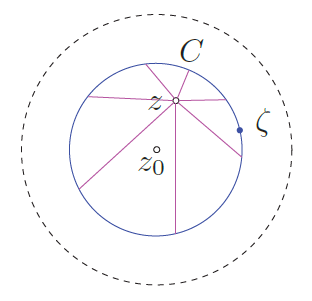
\includegraphics[width=0.3\textwidth]{./SaltChapter/fig-4-0-5}
\end{center}
%\caption{$\mathbb C$에 정의된 제곱급수의 수렴영역}
%\label{fig-4-0-3}
\end{figure*}

$|\zeta-z| = |\zeta-z_0-(z-z_0)| \ge
|\zeta-z_0| - |z-z_0| = r - |z-z_0|$이므로
\[
|R_n(z)| \le \left( \dfrac{|z-z_0|}r \right)^n \dfrac M{r-|z-z_0|} 
\stackrel{n\to\infty}{\longrightarrow} 0.
\]
따라서 제곱급수 $c_0 + c_1(z-z_0) + c_2(z-z_0)^2 + c_3(z-z_0)^3+ \cdots$는
$f(z)$로 수렴한다.
지금까지 결과로
\[
c_n = \dfrac1{2\pi i} \int_C \dfrac{f(\zeta)}{(\zeta-z_0)^{n+1}} d\zeta
\]
이 $|z-z_0|<r<R$인 $r$에서 성립한다는 것만을 보였다.
하지만 코시 적분정리를 사용하면 적분이 $r$에 무관함을 알 수 있고
$r\in (0,R)$이 다음을 만족하도록 선택할 수 있다.
\begin{itemize}
\item[(1)] $\dfrac{f(\cdot)}{(\cdot - z_0)^{n+1}}$이 
$0<|z-z_0|<R$인 뚫린 원판 $D_*(z_0,R)$에서 복소해석함수이다.
\item[(2)] $C$이외의 다른 경로로 중심이 $z_0$, 반지름 $\tilde r\in (0,R)$인 원 $\tilde C$를 잡으면
$C$와 $\tilde C$는 $D_*(z_0,R)$에서 호모토픽하다. 
\end{itemize}
이로써 증명이 완성된다. \hfill $\square$

한편 정리 \ref{thm-4-3}으로부터
\[
f(z) = \sum_{n=0}^\infty c_n(z-z_0)^n
\quad (|z-z_0| <R)
\]
로 정의하면 $n\ge0$에 대하여 $c_n = \dfrac{f^{(n)}(z_0)}{n!}$이다.
이상에서 적분으로 주어진 계수 $c_n$에 대한  다른 표현식을 얻었다.
하지만 임의의 원판에서 제곱급수를 전개할 때 계수는 유일하게 결정된다.
따라서 두 표현식은 같은 결과가 된다는 것을 기억하면 다음 결과를 얻는다.

\begin{salt_corollary}(테일러 급수) \label{coro-4-4}
\begin{itemize}
\item[(1)] $D$가 영역이고,
\item[(2)] $f:D\to \mathbb C$가 복소해석함수 이고,
\item[(3)] $z_0\in D$ 이면,
\end{itemize}
\[
f(z) = f(z_0) + \dfrac{f'(z_0)}{1!}(z-z_0) + \dfrac{f''(z_0)}{2!}(z-z_0)^ 2 
+ \cdots, \quad |z-z_0|<R.
\]
여기서 $R$은 $z_0$를 중심으로 하는 원판 중 영역 $D$에 속하는 가장 큰 열린집합의
반지름이다. 또한,
\begin{equation} \label{eq-4-2}
f^{(n)}(z_0) = \dfrac{n!}{2\pi i}\int_C {f(z)}{(z-z_0)^{n+1}}dz.
\end{equation}
\end{salt_corollary}
단, $C$는 $z_0$를 중심으로 하는 반지름 $r$ ($0<r<R$)인 원을 반시계방향으로 회전하는 경로이다.



%===[salt] 5장
% !TEX root = ../notes_template.tex

\chapter{조화함수}

마지막 장에서는 다음 내용을 다룬다.

\begin{itemize}
\item[(1)] 라플라스 방정식이라 불리는 편미분방정식의 해가 되는 실함수로서 조화함수를 공부한다.
\item[(2)] 복소해석함수의 실수부와 허수부는 조화함수가 되며
국소적으로 역도 성립한다. 단순연결 영역에서는 전체적으로 역이 성립한다.
\item[(3)] 조화함수와 복소해석함수의 상호관계로부터 도출되는 결과들, 특히
디리클레 방정식이라 불리는 경계값문제에 대한 결과를 살펴본다.
\end{itemize}

\section{조화함수란?}

\begin{salt_definition} \label{def-5-1}
$U$를 $\mathbb R^2$의 열린 부분집합이라고 하자.
함수 $u:U \to \mathbb R$가
$2$차까지의 도함수가 존재하고 연속이면서(줄여서 $u\in C^2$라 한다)
라플라스 방정식
\[
(\Delta u)(x,y) := \dfrac{\partial^2 u}{\partial x^2} (x,y) 
+ \dfrac{\partial^2 u}{\partial y^2} (x,y) = 0,
\quad
(x,y) \in U
\]
을 만족하면, {\bf 조화함수}(harmonic function)라고 한다.
\end{salt_definition}

\begin{salt_example}\label{example-5-1}
$U=\mathbb R^2$라 하자.
함수 $u: U\to \mathbb R$가 모든 $(x,y)\in \mathbb R^2$에서
$u(x,y) = x^2-y^2$로 주어지면,
\begin{align*}
 &\dfrac{\partial u}{\partial x} = 2x, \hphantom{-} \quad  \dfrac{\partial^2 u}{\partial x^2} = 2, \\
 &\dfrac{\partial u}{\partial y} = -2y, \quad   \dfrac{\partial^2 u}{\partial y^2} = -2
\end{align*}
이므로 $\dfrac{\partial^2 u}{\partial x^2} (x,y) 
+ \dfrac{\partial^2 u}{\partial y^2} (x,y) = 2-2=0$이다.
$\mathbb R^2$에서 $u\in C^2$이고 $\Delta u=0$이므로 $u$는 조화함수이다.
\hfill $\diamondsuit$
\end{salt_example}

물론 모든 함수가 조화함수는 아니다.

\begin{salt_example}\label{example-5-2}
$(x,y)\in \mathbb R^2$에서 $\tilde u(x,y) = x^2+y^2$으로 정의된 함수  $\tilde u$를 생각하면,
\[
\dfrac{\partial^2 \tilde u}{\partial x^2} (x,y) 
+ \dfrac{\partial^2 \tilde u}{\partial y^2} (x,y) = 2+2=4\ne 0.
\]
따라서 $\Delta \tilde u$는 $\mathbb R^2$의 모든 점에서 $0$이 되지 않기에
$\tilde u$는 $\mathbb R^2$의 어떤 열린 부분집합에서도 조화함수가 될 수 없다.
\hfill $\diamondsuit$
\end{salt_example}

\begin{salt_exercise}\label{ex-5-1}
다음 함수 $u$가 주어진 열린집합 $U$에서 조화함수임을 보여라.
\begin{itemize}
\item[(1)] $u(x,y) = \log (x^2+y^2)$, $U = \mathbb R^2\setminus \{(0,0)\}$
\item[(2)] $u(x,y) = e^x\sin y$, $U=\mathbb R^2$.
\end{itemize}
\end{salt_exercise}

\begin{salt_exercise}\label{ex-5-2}
열린집합 $U$에 정의된 모든 조화함수의 집합 $\Har(U)$는
점별 연산에 대하여 실벡터공간을 이룸을 보여라.
\end{salt_exercise}

\begin{salt_exercise}\label{ex-5-3}식
조화함수의 점별 곱으로 만든 함수도 조화함수가 되는가?
\end{salt_exercise}

{\bf 왜 조화함수에 신경써야 하는가?}

조화함수는 라플라스 방정식을 만족하기 때문에 중요한데,
라플라스 방정식은 여러가지 이유 중 다음 두 가지 때문에 특히 중요하다.
\begin{itemize}
\item[(1)] 라플라스 방정식은 편미분방정식(PDE)의 3가지 유형 중에서 
타원형 방정식이라는 중요한 유형에 속한다.
\begin{center}
\begin{tabular}{ |c|c| } 
 \hline
PDE 유형 & 예 \\ \hline \hline
타원형 & 라플라스 방정식 
$\dfrac{\partial^2 u}{\partial x^2} 
+ \dfrac{\partial^2 u}{\partial y^2} =0$ \\[1ex] \hline
포물형 & 확산 방정식 $\dfrac{\partial u}{\partial t} 
+ \dfrac{\partial^2 u}{\partial x^2} =0$ \\[1ex] \hline
쌍곡형 & 파동 방정식 $\dfrac{\partial^2 u}{\partial t^2} 
- \dfrac{\partial^2 u}{\partial x^2} =0$ \\[0.5ex]
\hline
\end{tabular}
\end{center}
\item[(2)] 라플라스 방정식은 많은 응용분야에서 사용된다.
다음과 같이 물리학에서 사용되는 예를 살펴보자.
유체역학에서 유체흐름의 ``속도 포텐셜(velocity potential)''은
라플라스 방정식을 만족한다. 한편, 정전기학에서는
정전기 전위(electronic potential)가 라플라스 방정식을 만족한다.
라플라스 방정식은 확률과정(stochastic process)과도 중요한 연결고리를 갖는다.
아래에서 이를 간단히 알아보자.
열린 단위원판 $\mathbb D:= \{z\in \mathbb C\,:\, |z|<1\}$을 생각하자.
입자가 한점 $z\in\mathbb D$에서 브라운 운동을 따른다고 하자.
(예를 들면, 무작위 운동을 만드는 물분자에 의해 충격받는 물 속의
꽃가루를 생각하자.)
직관적으로 무작위 운동으로 언젠가는 입자가 $\mathbb D$의 경계 
$\mathbb T:= \{ z\in \mathbb C \,:\, |z|=1 \}$를 벗어난다.
$z$에서 출발한 입자가 처음으로 단위원 $\mathbb T$를 벗어나는 
점을 $\zeta_z$라고 하자. 그러면 확률변수 $\zeta_z$는 단위원 위에 표시된다.
그림 \ref{fig-5-1}을 참고하라.
\begin{figure}[h!]
\begin{center}
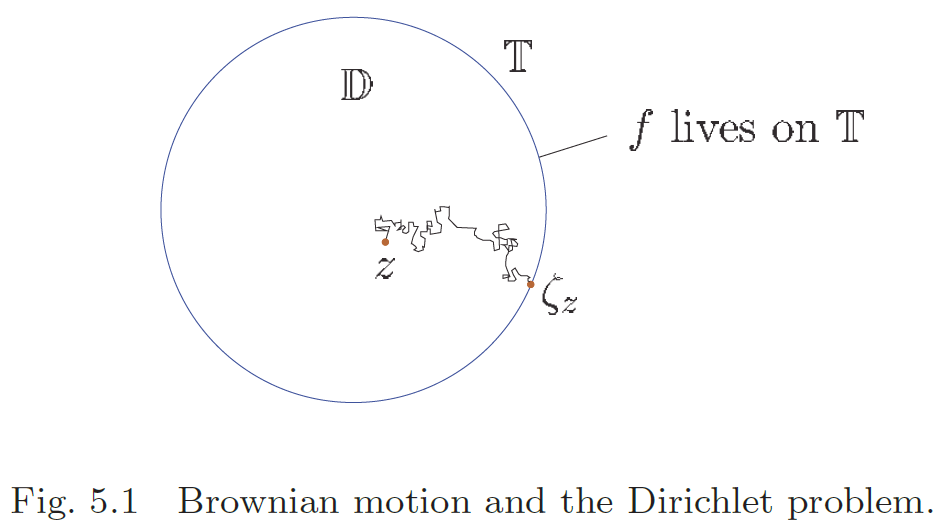
\includegraphics[width=0.6\textwidth]{./SaltChapter/fig-5-1}
\end{center}
\caption{브라운 운동과 디리클레 문제}
\label{fig-5-1}
\end{figure}
이제 연속함수 $f:\mathbb T \to \mathbb R$이 주어졌다고 하자.
그러면 $f(\zeta_z)$를 $\mathbb T$에 정의된 실수 값을 갖는 확률변수로 생각할 수 있다.
그 기댓값을 $\mathbb E(f(\zeta_z))$으로 표기하자.
이 값은 어디에서 출발하는지에 따라 달라진다. 즉, $z$에 의존하는 값이다.
$u:\mathbb D \to \mathbb R$을 $u(z) =\mathbb E(f(\zeta_z))$ ($z\in \mathbb D$)로 
정의하자. 이 때, $u$는 조화함수이고 실제로 디리클레 문제의 해가 됨이 알려져 있다.
이는 경계값 문제로 경계 $\mathbb T$에서 함수 $f:\mathbb T \to \mathbb R$가 
주어져 있을 때, $\mathbb T$의 내부 $\mathbb D$에서는 라플라스 방정식을 만족하고
경계 $\mathbb T$까지 연속함수로 확장되어 $f$와 일치하는 함수 $u$를 찾는 문제이다.
\[
\begin{cases}
\Delta u = 0, & \mathbb D\text{\,에서},\\
u\big|_{\mathbb T}= f.
\end{cases}
\]
\end{itemize}

\section{조화함수와 복소해석함수의 연결고리는 무엇인가?}

조화함수는 단지 실해석의 영역에 속해야 하는 것처럼 보일 수 있다.
이 절에서는 복소해석학에 대한 연구를 충분히 정당화할 수 있는 두가지 결과를 알아볼 것이다.
개략적으로 말하면, 열린집합에 정의된 조화함수는 국소적으로 복소해석함수의 실수부라는 
조건과 동치이다.








%====[풀 이]====================
\begin{appendices}
%===[salt] 0장, 1장
% !TEX root = ./CA_solution.tex

\chapter*{연습문제 풀이}

\section*{머리말 - 연습문제 풀이}

\subsection*{연습문제 \ref{ex-0-1}}

$0$에서 $f'$의 미분이 존재하고 그 값이 $L$이라고 가정하자.
$\epsilon:=1>0$으로 잡으면, $0<|x-0|<\delta$이면
\[
\left| \dfrac{f'(x) - f'(0)}{x-0} - L\right| <\epsilon
\]
을 만족하는 $\delta>0$가 존재한다.
특히 $x:=\delta/2$로 잡으면
$0<|x-0| = \delta/2 < \delta$이므로
\begin{equation} \label{eq-5-5}
\left| \dfrac{f'(x) - f'(0)}{x-0} - L\right|
= \left| \dfrac{2(\delta/2) - 0}{(\delta/2)-0} - L\right| 
= |2-L| < \epsilon.
\end{equation}
한편 $x:=-\delta/2$로 잡아도
$0<|x-0| = \delta/2 < \delta$이므로
\begin{equation} \label{eq-5-6}
\left| \dfrac{f'(x) - f'(0)}{x-0} - L\right|
= \left| \dfrac{-2(-\delta/2) - 0}{(-\delta/2)-0} - L\right| 
= |2+L| < \epsilon.
\end{equation}
식 \eqref{eq-5-5}와 \eqref{eq-5-6}으로부터
실수 절대값에 대한 삼각부등식을  이용하면
\[
4 = |2+L+2-L| \le |2+L| + |2-L|
<\epsilon + \epsilon = 2\epsilon = 2
\]
가 되어 모순이다.
따라서 $f'$은 $0$에서 미분이 불가능하다.

\section*{1장 - 연습문제 풀이}

\subsection*{연습문제 \ref{ex-1-1}}

$(x,y) \ne 0$이므로, 
$x$, $y$ 중 적어도 하나는 $0$이 아니다.
따라서 $x^2+y^2\ne 0$이고,
\[
\left( \dfrac x{x^2+y^2}, \dfrac{-y}{x^2+y^2} \right) \in \mathbb R^2.
\]
또한,
\begin{align*}
(x,y) \cdot & \left( \dfrac x{x^2+y^2}, \dfrac{-y}{x^2+y^2} \right) \\
&=\left( x\cdot \dfrac x{x^2+y^2} - y\cdot \left( \dfrac{-y}{x^2+y^2} \right),
x\cdot \left(\dfrac{-y}{x^2+y^2}\right) + y\cdot  \dfrac{x}{x^2+y^2} \right) \\
&= \left( \dfrac{x^2+y^2}{x^2+y^2}, \dfrac{-xy + xy}{x^2+y^2} \right) = (1,0).
\end{align*}
따라서 $(x,y) \ne(0,0)$에 대하여
$
(x,y)^{-1} = \left(\dfrac x{x^2+y^2}, \dfrac{-y}{x^2+y^2} \right)
$이다.

\subsection*{연습문제 \ref{ex-1-2}}

$\theta \in \left(-\dfrac{\pi}2, \dfrac\pi2 \right)$이므로,
$\tan \theta \in \mathbb R$이고,

\begin{align*}
\dfrac1{1-i\tan\theta}
&= \dfrac1{1^2+(\tan\theta)^2} 
+ i\left( \dfrac{\tan\theta}{1^2 + (\tan\theta)^2} \right) \\
&= \dfrac{(\cos\theta)^2}{(\cos\theta)^2 + (\sin\theta)^2}
+ i\left( \dfrac{\dfrac{\sin\theta}{\cos\theta}\cdot(\cos\theta)^2}
{(\cos\theta)^2 + (\sin\theta)^2} \right) \\
&= \dfrac{(\cos\theta)^2}1 + i \dfrac{(\sin\theta)(\cos\theta)}1
= (\cos\theta)^2 + i(\sin\theta)(\cos\theta).
\end{align*}
따라서
\begin{align*}
\dfrac{1+i\tan\theta}{1-i\tan\theta}
&= (1+i\tan\theta)( (\cos\theta)^2 + i(\sin\theta)(\cos\theta) ) \\
&= (\cos\theta)^2 - \dfrac{\sin\theta}{\cos\theta} \cdot
(\sin\theta)(\cos\theta) \\
&\quad\quad + \left(
(\sin\theta)(\cos\theta) + \dfrac{\sin\theta}{\cos\theta} \cdot (\cos\theta)^2
\right) \\
&= (\cos\theta)^2 - (\sin\theta)^2 + i2(\sin\theta)(\cos\theta)
= \cos(2\theta) + i\sin(2\theta).
\end{align*}

\subsection*{연습문제 \ref{ex-1-3}}

$P\subset \mathbb C$가 $\mathbb C$의 양의 부분집합이라고 하자.
그러면, $i\ne0$이므로 조건 (P3)에 의해
$i\in P$이거나 ($i\ne P$이고 $-i\in P$)이다.
조건 (P2)에서
\begin{equation}\label{eq-5-7}
-1 = i\cdot i = (-i)\cdot (-i) \in P
\end{equation}
이고, 다시 (P2)에서
\begin{equation}\label{eq-5-8}
1 = (-1)\cdot(-1) \in P
\end{equation}
가 된다. 
그런데 $1\ne0$이고
$x=1$이라고 하면 (P3)에서
\eqref{eq-5-7}, \eqref{eq-5-8}\은 동시에 만족될 수 없기에 모순이다.

\subsection*{연습문제 \ref{ex-1-4}}

아래 그림 \ref{fig-5-2}\와 같다.

\begin{figure}[h!]
\begin{center}
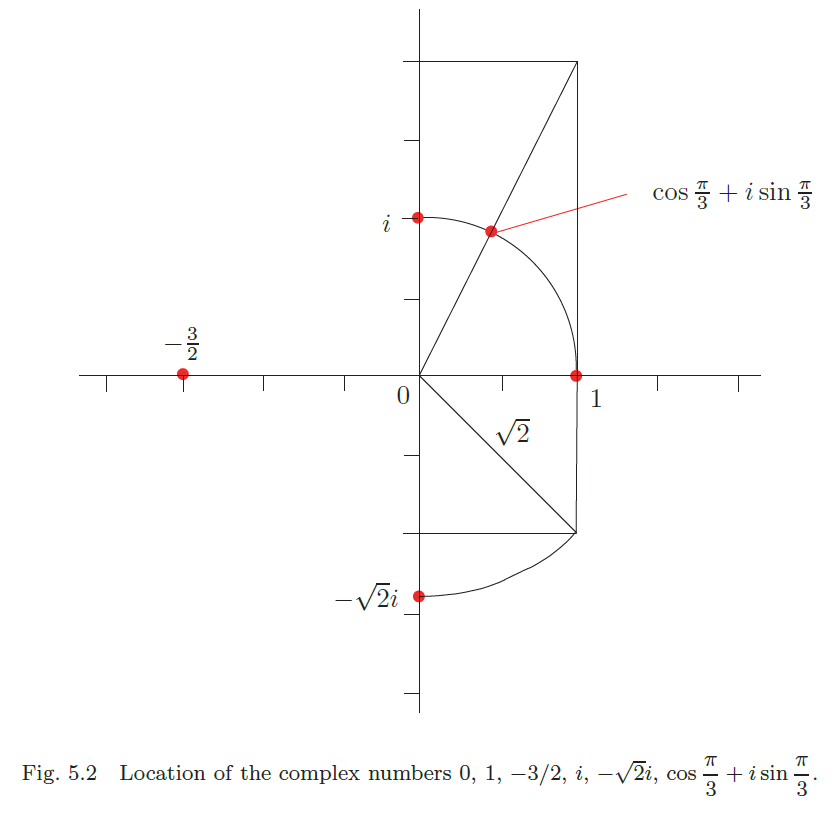
\includegraphics[width=0.7\textwidth]{./figs/fig-5-2}
\end{center}
\caption{복소수 $0$, $1$, $-3/2$, $i$, $-\sqrt{2}i$,
$\cos\dfrac\pi3 + i\sin\dfrac\pi3$의 위치}
\label{fig-5-2}
\end{figure}

\subsection*{연습문제 \ref{ex-1-5}}

$\theta\in\mathbb R$에 대하여
$(\cos\theta + i\sin\theta)^3 = \cos(3\theta) + i\sin(3\theta)$이다.
\begin{align*}
(\cos\theta + i\sin\theta)^3 
&= (\cos\theta + i\sin\theta)\left(
(\cos\theta)^2 - (\sin\theta)^2 + i2(\cos\theta)(\sin\theta) \right) \\
&= (\cos\theta)\left( (\cos\theta)^2 - (\sin\theta)^2 \right)
- (\sin\theta)2(\cos\theta)(\sin\theta)  \\
&\quad\quad + i(\ \cdots\ ).
\end{align*}
따라서 양변의 실수부가 같다는 것을 이용하면,
\begin{align*}
\cos(3\theta) &= \Re((\cos\theta + i\sin\theta)) \\
&=(\cos\theta)\left( (\cos\theta)^2 - (\sin\theta)^2 \right)
- 2(\cos\theta)(\sin\theta)^2 \\
&= (\cos\theta)\left( (\cos\theta)^2 - 1 + (\cos\theta)^2 \right)
- 2(\cos\theta)(1-\cos\theta)^2 \\
&= (\cos\theta)^3 - \cos\theta  + (\cos\theta)^3 - 2\cos\theta + 2(\cos\theta)^3 \\
&= 4(\cos\theta)^3 - 3\cos\theta
\end{align*}
다른 방법으로, 이항정리 공식
$(a+b)^n = \Sum_{k=0}^n \disp{n \choose k} a^kb^{n-k}$이
복소수 $a,b \in \mathbb C$와 자연수 $n\in \mathbb N$에 대하여
성립한다는 것을 이용하면,
\begin{align*}
\cos(3\theta) &= \Re((\cos\theta + i\sin\theta)) \\
&= \Re ( (\cos\theta)^3 + 3(\cos\theta)^2(i\sin\theta) 
+ 3(\cos\theta)(i\sin\theta)^2 + (i\sin\theta)^3) \\
&= (\cos\theta)^3 - 3(\cos\theta)(\sin\theta)^2 \\
&= 4(\cos\theta)^3 - 3\cos\theta.
\end{align*}

\subsection*{연습문제 \ref{ex-1-6}}

$1+i = \sqrt{2}\left(\dfrac1{\sqrt{2}} + i\dfrac1{\sqrt{2}}\right)
= \sqrt{2}\left( \cos\dfrac\pi4 + i\sin \dfrac\pi4 \right)$로 쓸 수 있다.
따라서,
\begin{align*}
(1+i)^{10}
&= (\sqrt{2})^{10} \left( \cos\dfrac\pi4 + i\sin \dfrac\pi4 \right)^{10}
= 2^5 \left( \cos\left(10\cdot \dfrac\pi4\right) 
+ i\sin \left(10\cdot \dfrac\pi4\right) \right) \\
&= 32 \left( \cos\left(2\pi+\dfrac\pi2\right) 
+ i\sin \left(2\pi+\dfrac\pi2\right) \right) \\
&=32 \left( \cos\left(\dfrac\pi2\right) + i\sin \left(\dfrac\pi2\right) \right) 
= 32(0+i\cdot 1) = 32i.
\end{align*}

\subsection*{연습문제 \ref{ex-1-7}}

$2+i$가 실수축의 양의 방향과 이루는 각도는 $\tan^{-1}(1/2)$이고
$3+i$가 실수축의 양의 방향과 이루는 각도는 $\tan^{-1}(1/3)$이다.
따라서, $(2+i)(3+i)$가 실수축의 양의 방향과 이루는 각도는 
$\tan^{-1}(1/2) + \tan^{-1}(1/3)$이다.
한편,
\[
(2+i)(3+i) = 6 - 1 + i(2+3) = 5 + 5i
\]
이므로 $(2+i)(3+i)$가  실수축의 양의 방향과 이루는 각도는
\[
\tan^{-1} (5/5) = \tan^{-1} 1 = \pi/4
\]
이다. 결론적으로, 
$\dfrac\pi4 = \tan^{-1}\dfrac12 + \tan^{-1}\dfrac13$이다.

\subsection*{연습문제 \ref{ex-1-8}}

정삼각형의 꼭지점  $A$, $B$, $C$의 위치가 
반시계방향의 순서로 복소수 $z_A$, $z_B$, $z_C$에 있다고 하자.
$\ell(AC) = \ell(AB)$이고 $\angle CAB=\pi/3$이므로,
\begin{equation}\label{eq-5-9}
z_C - z_A = \left( \cos\dfrac\pi3 + i\sin\dfrac\pi3 \right)(z_B - z_A).
\end{equation}
귀류법을 쓰기위해 $p,q,m,n\in\mathbb Z$가 
\[
z_C - z_A = p+iq, \quad
z_B - z_A = m+in
\]
을 만족한다고  하자.
그러면, 식 \eqref{eq-5-9}에서
$p+iq = \left(\dfrac12 + \dfrac{\sqrt{3}}2i\right)(m+in)$을 다시 쓰면,
\begin{align}
p &= \dfrac m2 - \dfrac{\sqrt{3}}2n, \label{eq-5-10} \\
q &= \dfrac{m\sqrt{3}}2 + \dfrac n2. \label{eq-5-11}
\end{align}
식 \eqref{eq-5-10}에 $-n$을 곱하고,
식 \eqref{eq-5-11}에 $m$을 곱하여 더하면,
\[
qm - pn = \dfrac{\sqrt{3}}2 (m^2 + n^2)
\]
을 얻는다.
그런데 $m^2+n^2 \ne0$이므로 ($z_B \ne z_A$이므로),
\[
\sqrt{3} = \dfrac{2(qm-pn)}{m^2+n^2} \in \mathbb Q
\]
를 얻어 모순이 생긴다.

\subsection*{연습문제 \ref{ex-1-9}}

$-1 = 1 \cdot (\cos \pi + i \sin \pi)$로 쓸 수 있다.
$w = \rho(\cos\alpha + i\sin\alpha)$가 
\[
w^4 = \rho^4(\cos(4\alpha) + i\sin(4\alpha)) = 1 \cdot (\cos \pi + i \sin \pi)
\]
를 만족해야 하므로,
$\rho^4 = 1$에서 $\rho=1$이다.
또한, $4\alpha \in \{ \pi, \pi\pm2\pi, \pi\pm4\pi, \ldots\}$에서
\[
\alpha \in \left\{ \dfrac\pi4, \dfrac\pi4\pm\dfrac\pi2, \dfrac\pi4\pm\pi,\ldots
\right\}.
\]
따라서 $ w = \rho(\cos\alpha + i\sin\alpha) = 1\cdot((\cos\alpha + i\sin\alpha) $는
다음 집합에 속한다.
\begin{align*}
&\left\{ \cos\dfrac\pi4+i\sin\dfrac\pi4, \cos\dfrac{3\pi}4+i\sin\dfrac{3\pi}4, 
\cos\dfrac{5\pi}4+i\sin\dfrac{5\pi}4, \cos\dfrac{7\pi}4+i\sin\dfrac{7\pi}4
\right\} \\
&\qquad\quad\quad = \left\{ \dfrac{1+i}{\sqrt{2}},  \dfrac{-1+i}{\sqrt{2}},
 \dfrac{-1-i}{\sqrt{2}},  \dfrac{1-i}{\sqrt{2}} \right\}.
\end{align*}

네 개의 해를 복소평면에 그려보면 그림 \ref{fig-5-3}\과 같다.

\begin{figure}[h!]
\begin{center}
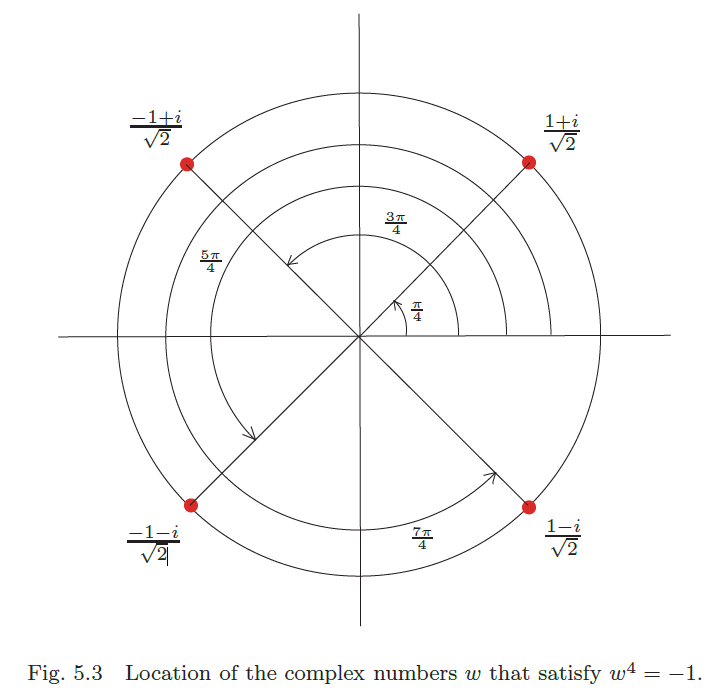
\includegraphics[width=0.6\textwidth]{./figs/fig-5-3}
\end{center}
\caption{$w^4=-1$을 만족하는 복소수 $w$의 위치}
\label{fig-5-3}
\end{figure}

\subsection*{연습문제 \ref{ex-1-10}}

방정식으로부터
\[
0=z^6 -z^3-2 = (z^3)^2 -2z^3 +z^3 -2 = (z^3-2)(z^3+1)
\]
이므로
$z^3=2$ 또는 $z^3=-1$이다.
$z^3=2$를 만족하는 해를 구하면
\[
z\in \left\{ \sqrt[3]{2} \left( \cos\dfrac{2\pi}3 + i\sin\dfrac{2\pi}3\right),
\sqrt[3]{2} \left( \cos\dfrac{4\pi}3 + i\sin\dfrac{4\pi}3\right), 
\sqrt[3]{2} \right\}
\]
로부터 
\[
z\in \left\{ \sqrt[3]{2} \left( - \dfrac12+ i\dfrac{\sqrt{3}}2\right),
\sqrt[3]{2} \left( -\dfrac12 - i\dfrac{\sqrt{3}}2\right), 
\sqrt[3]{2} \right\}
\]
이다. 한편, $z^3=-1$의 해는
\[
z\in\left\{ \cos\dfrac\pi3 + i\sin\dfrac\pi3, \cos\pi + i\sin\pi,
\cos\dfrac{5\pi}3 + i\sin\dfrac{5\pi}3 \right\}
\]
로부터 
\[
z\in \left\{ \dfrac12+ i\dfrac{\sqrt{3}}2, -1,
\dfrac12 - i\dfrac{\sqrt{3}}2 \right\}
\]
이다. 결론적으로
$z^6 - z^3-2=0$일 필요충분조건은 [$z^3=2$ 또는 $z^3=-1$]이다.
즉,
\begin{align*}
z\in & \left\{ \sqrt[3]{2} \left( - \dfrac12+ i\dfrac{\sqrt{3}}2\right),
\sqrt[3]{2} \left( -\dfrac12 - i\dfrac{\sqrt{3}}2\right), 
\sqrt[3]{2} \right\}\\
&\bigcup \left\{ \dfrac12+ i\dfrac{\sqrt{3}}2, -1,
\dfrac12 - i\dfrac{\sqrt{3}}2 \right\}.
\end{align*}
따라서 구하는 해는
\[
z\in \left\{ \sqrt[3]{2} \left( - \dfrac12+ i\dfrac{\sqrt{3}}2\right),
\sqrt[3]{2} \left( -\dfrac12 - i\dfrac{\sqrt{3}}2\right), 
\sqrt[3]{2},
\dfrac12+ i\dfrac{\sqrt{3}}2, -1,
\dfrac12 - i\dfrac{\sqrt{3}}2 \right\}.
\]

\subsection*{연습문제 \ref{ex-1-11}}

$\omega^3=1$을 만족하는 $\omega\in\mathbb C \setminus \mathbb R$을 생각하자.
그러면, $(\omega-1)(\omega^2+\omega+1)=0$이고,
$\omega\ne1$이므로 $\omega^2+\omega+1=0$이다.
따라서,
\begin{align*}
((b-a)\omega &+(b-c))((b-a)\omega^2+b-c) \\
&= (b-a)^2\omega^3 + (b-a)(b-c)(-1) + (b-c)^2 \\
&= (b-a)^2\cdot 1 + (b-a)(b-c)(-1)  + (b-c)^2 \\
&= (b-a)(b-a-b+c) + (b-c)^2 \\
&=(bc-ca-ab+a^2+b^2-2bc+c^2 \\
&= a^2+b^2+c^2 -ab - bc - ca = 0.
\end{align*}
따라서 $(b-a)\omega = c-b$이거나 $(b-a)\omega^2 = c-a$이다.
두번째 식은 $(b-a)\omega^3 = (c-a)\omega$와 동치이므로
$(c-b)\omega = b-a$이다.
이로부터 $|b-a|=|c-b|$를 얻고
$a$와 $b$, $a$와 $c$를 잇는 두 선분의 사잇각은 $\pi/3$이다.
그림 \ref{fig-5-4}\를 참고하라.

\begin{figure}[h!]
\begin{center}
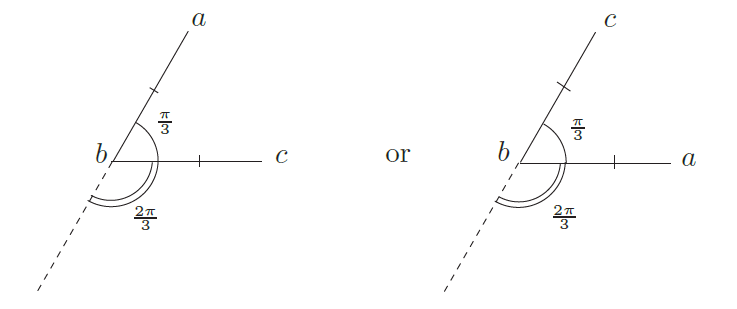
\includegraphics[width=0.6\textwidth]{./figs/fig-5-4}
\end{center}
\caption{정삼각형을 이루는 세 점 $a$, $b$, $c$}
\label{fig-5-4}
\end{figure}

두 가지 그림 모두 세 점 $a$, $b$, $c$는 정삼각형을 이룬다.
 $a$, $b$, $c$가 실수인 경우는 한점 $r\in\mathbb R$로 모이게 되어
 $a=b=c=(=r)$이 되어 실수의 경우도 원하는 결과를 얻는다.

\subsection*{연습문제 \ref{ex-1-12}}

$\omega\in\mathbb C\setminus \mathbb R$이 $\omega^3=1$을 만족한다고 하자.
$(\omega-1)(\omega^2+\omega+1)=0$이고,
$\omega\ne1$이므로 $\omega^2+\omega+1=0$이다.
또한, $1+\omega^2+\omega^4 = 1+ \omega^2 + \omega\cdot\omega^3 =
1+ \omega^2 + \omega = 0$이므로,
\[
(1+1)^{3n} + (1+\omega)^{3n} + (1+\omega^2)^{3n}
= \Sum_{k=0}^{3n} {3n \choose k} (1+\omega^k + \omega^{2k}).
\]
그런데,
\begin{align*}
(1+\omega^k + \omega^{2k})
&= \begin{cases}
1+1+1, & k\equiv 0 \mod 3, \\
1+\omega + \omega^2, & k\equiv 1 \mod 3, \\
1+\omega^2 + \omega^4,& k\equiv 2 \mod 3
\end{cases} \\
&=\begin{cases}
3, & k\equiv 0 \mod 3, \\
0, & k\equiv 1 \mod 3, \\
0, & k\equiv 2 \mod 3.
\end{cases}
\end{align*}
에서
\[
(1+1)^{3n} + (1+\omega)^{3n} + (1+\omega^2)^{3n}
= 3\cdot \left(
{3n \choose 0} + {3n \choose 3} + \cdots + {3n \choose 3n} \right).
\]
다른 방법으로 보면,
\begin{align*}
(1+1)^{3n} + (1+\omega)^{3n} + (1+\omega^2)^{3n}
&= 2^{3n} + (-\omega^2)^{3n} +  (-\omega)^{3n} \\
&= 2^{3n} + (-1)^n + (-1)^n \\
&= 2^{3n} + 2\cdot(-1)^n
\end{align*}
이므로 원하는 결과를 얻는다.

\subsection*{연습문제 \ref{ex-1-13}}

\begin{figure}[h!]
\begin{center}
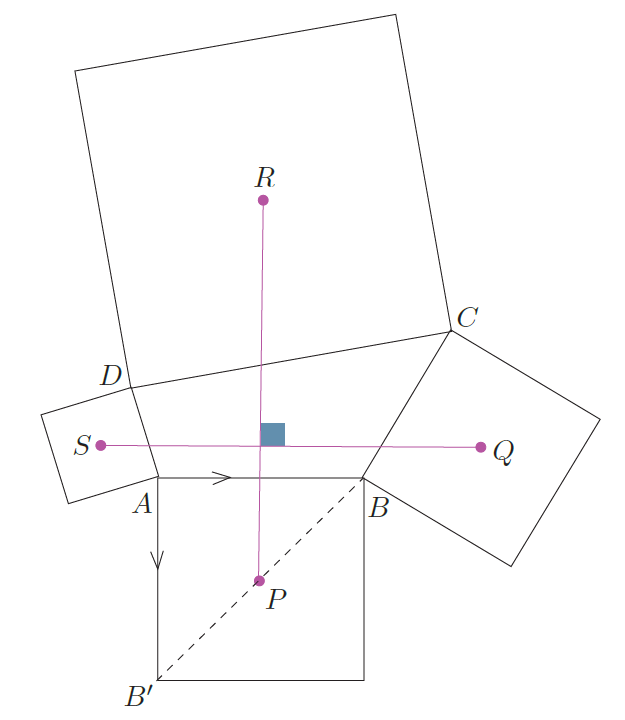
\includegraphics[width=0.6\textwidth]{./figs/fig-5-5}
\end{center}
\caption{$RP$와 $SQ$는 길이가 같고 수직으로 만난다}
\label{fig-5-5}
\end{figure}

그림 \ref{fig-5-5}\와 같이
평면위의 네 점 $A$, $B$, $C$, $D$를 복소수 $a$, $b$, $c$, $d$에 각각 대응시키자.
$AB'$은  $A$를 중심으로 하여 $AB$를 반시계방향으로 $90^\circ$회전한 것이므로
$B'$은 복소수 $a-i(b-a)$에 대응된다.
$P$는 $BB'$의 중점이므로 다음 복소수에 대응된다.
\[
\dfrac{a+b-i(b-a)}2.
\]
같은 방법으로 $Q$, $R$, $S$는 각각 다음 복소수에 대응된다.
\[
\dfrac{b+c-i(c-b)}2, \quad
\dfrac{c+d-i(d-c)}2, \quad
\dfrac{d+a-i(a-d)}2.
\]
점 $P$, $Q$, $R$, $S$에 대응되는 복소수를 각각
$p$, $q$, $r$, $s$라 하면,
\begin{align*}
i(q-s) &= i \left(
\dfrac{b+c-i(c-b)}2 - \dfrac{d+a-i(a-d)}2 \right) \\
&= \dfrac{-b+c-a+d+i(b+c-d-a)}2 \\
&= \dfrac{-a-b+i(b-a)}2 + \dfrac{c+d-i(d-c)}2 = -p+r
\end{align*}
이므로, $|q-s| = |p-r|$이 되어 $\ell(QS) = \ell(PR)$이다.
또한, $i$를 곱하는 것은 원점을 중심으로 $90^\circ$ 회전을 의미하기 때문에
$PR\perp QS$이다.

\subsection*{연습문제 \ref{ex-1-14}}

실수 $x_1, x_2, y_1, y_2$에 대하여
$z_1 = x_1 + iy_1$, $z_2 = x_2 + iy_2$라 하자.
그러면 $z_1z_2 = x_1x_2 - y_1y_2 = i(x_1y_2+y_1x_2)$이고,
\begin{align*}
|z_1z_2|^2 &=  (x_1x_2 - y_1y_2)^2 + (x_1y_2 + y_1x_2)^2 \\
&= x_1^2x_2^2 - \cancel{2x_1x_2y_1y_2} + y_1^2y_2^2
+ x_1^2y_2^2 + \cancel{2x_1y_2y_1x_2} + y_1^2x_2^2 \\
&=x_1^2(x_2^2+y_2^2) + y_1^2(y_2^2+x_2^2)
= (x_1^2+y_1^2)(x_2^2+y_2^2) \\
&= |z_1|^2|z_2|^2.
\end{align*}
$|z_1|$, $|z_2|$, $|z_1z_2|$는 모두 음이 아닌 실수 이므로
$|z_1||z_2| = |z_1||z_2|$가 성립한다.

\subsection*{연습문제 \ref{ex-1-15}}

$z=x+iy$ ($x,y\in\mathbb R$)이라 하자. 그러면,
\[
\overline{(\bar z)} = \overline{x-iy}
= x - i(-y) = x+iy = z.
\]
또한, 
\[
z\bar z = (x+iy)(x-iy) = x^2+y^2 + i(- xy + xy)
= x^2+y^2 = |z|^2.
\]
끝으로,
\begin{align*}
\dfrac{z + \bar z}2 &= \dfrac{x+\cancel{iy}+ x -\cancel{iy}}2
= \dfrac{2x}2 = x =\Re(z), \\
\dfrac{z - \bar z}{2i} &= \dfrac{\cancel{x}+iy - \cancel{x} +iy}{2i}
= \dfrac{2iy}{2i} = y = \Im(z).
\end{align*}

\subsection*{연습문제 \ref{ex-1-16}}

$z = x+iy$ ($x,y\in\mathbb R$)이라 하면,
\begin{align*}
|z| &= |x+iy| = \sqrt{x^2+y^2} = \sqrt{x^2+(-y)^2} = |x-iy| = |\bar z|, \\
|\Re(z)| & =  |x| = \sqrt{x^2} \le  \sqrt{x^2+y^2} = |x+iy| = |z|, \\
|\Im(z)| &= |y| = \sqrt{y^2} \le  \sqrt{x^2+y^2} = |x+iy| = |z|.
\end{align*}

$\bar z$는 $z$를 실수축에 대칭시켜 얻어지며,
$0\in\mathbb R$이므로 원점과 $z$와의 거리는 $\bar z$와의 거리와 같다.
즉, $ |z| = |\bar z|$.
부등식 $|\Re(z)| \le|z|$와 $|\Im(z)|\le |z|$는 
아래 그림에서 직각삼각형에서 빗변의 길이가 가장 길다는 것을 의미한다.

\begin{figure*}[h!]
\begin{center}
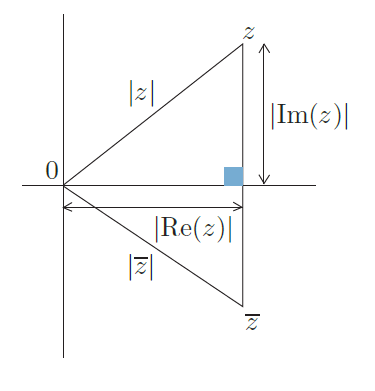
\includegraphics[width=0.3\textwidth]{./figs/fig-s-0-1}
\end{center}
%\caption{$RP$와 $SQ$는 길이가 같고 수직으로 만난다}
%\label{fig-5-5}
\end{figure*}

\subsection*{연습문제 \ref{ex-1-17}}

우선 $|\bar az| = |\bar a||z| = |a||z| <1\cdot 1 =1$이므로, $\bar az \ne 1$이고,
\begin{align*}
\dfrac{z-a}{1-\bar az}\cdot \overline{\left(\dfrac{z-a}{1-\bar az}\right)}
&= \dfrac{z-a}{1-\bar az}\cdot \dfrac{\bar z-\bar a}{1-a\bar z}
= \dfrac{z\bar z - a\bar z - \bar a z+a\bar a}{1-a\bar z - \bar a z + a\bar a z \bar z} \\
&= \dfrac{|z|^2 - a\bar z - \bar a z + |a|^2}{1-a\bar z - \bar a z + |a|^2|z|^2} \\
&= \dfrac{1 - a\bar z - \bar a z + |a|^2|z|^2+|z|^2+|a|^2-1-|a|^2|z|^2}
{1-a\bar z - \bar a z + |a|^2|z|^2} \\
&= 1 + \dfrac{|z|^2+|a|^2-1-|a|^2|z|^2}{1-a\bar z - \bar a z + |a|^2|z|^2} \\
&= 1 + \dfrac{|z|^2+|a|^2-1-|a|^2|z|^2}{|1- \bar a z|^2} \\
&= 1 -  \dfrac{(1-|z|^2)(1-|a|^2)}{|1- \bar a z|^2}.
\end{align*}
따라서
$\left| \dfrac{z-a}{1-\bar az} \right|^2 = 1 -
\underbrace{\dfrac{(1-|z|^2)(1-|a|^2)}{|1- \bar a z|^2}}_{\ge0\ (|z|<1, |a|<1\text{ 이므로})}
\le 1-0 = 1$.

\subsection*{연습문제 \ref{ex-1-18}}

$w\in\mathbb C$가 $p(w)=0$, 즉,
$c_0 + c_1w + \cdots + c_dw^d=0$을 만족한다고 하자. 
그러면,
\[
\overline{c_0 + c_1w + \cdots + c_dw^d} = \bar 0 = 0
\]
이고, 모든 $c_k$ ($0\le k\le d$)가 실수이므로
\begin{align*}
0 & = \overline{c_0 + c_1w + \cdots + c_dw^d} 
= \overline{c_0} + \overline{c_1w} + \cdots + \overline{c_dw^d} \\
&= \overline{c_0} + \overline{c_1}\overline{w} + \cdots + \overline{c_d}\overline{w^d}
= c_0 + c_1\overline{w} + \cdots + c_d(\bar w)^d.
\end{align*}
마지막 등식에서 
\[
\overline{w^k} = \underbrace{\overline{w\cdots w}}_{k\text{번}}
= \underbrace{\bar w \cdots \bar w}_{k\text{번}}
= (\bar w)^k,
\quad 1\le k \le d
\]
를 사용하였다.
따라서, $0=c_0 + c_1\overline{w} + \cdots + c_d(\bar w)^d = p(\bar w)$.

\subsection*{연습문제 \ref{ex-1-19}}

$a = |a|(\cos\alpha + i\sin\alpha)$, 
$b = |b|(\cos\beta + i\sin \beta)$라고 하자.
단, $\alpha, \beta \in [0,2\pi)$. 그러면,
\begin{align*}
a\bar b &= |a|(\cos\alpha + i\sin\alpha)\cdot
|b|(\cos\beta - i\sin \beta) \\
&=|a||b|(\cos\alpha + i\sin\alpha)(\cos\beta - i\sin \beta)
\end{align*}
이고 $\Im(a\bar b) = |a||b|(-(\cos\alpha)(\sin\beta) + (\sin\alpha)(\cos\beta))
= |a||b|\sin(\alpha-\beta)$.
$0$, $a$, $b$를 꼭지점으로 하는 $\Delta OAB$의 면적은
($O\equiv 0$, $A\equiv a$, $B\equiv b$)
\[
\dfrac12 \ell(OA)\ell(OB) \cdot \sin \angle AOB
= \dfrac12 |a|\cdot |b| \cdot |\sin(\alpha-\beta)|
= \dfrac12 |\Im(a\bar b)| = \left| \dfrac{\Im(a\bar b)}2\right|.
\]

\begin{figure}[h!]
\begin{center}
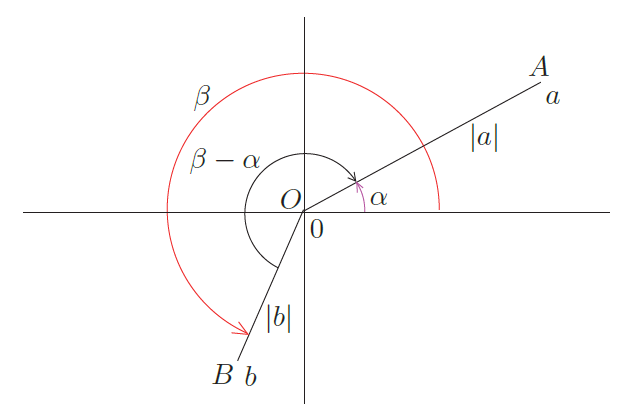
\includegraphics[width=0.7\textwidth]{./figs/fig-5-6}
\end{center}
\caption{$0$, $a$, $b$를 꼭지점으로 하는 $\Delta OAB$의 면적}
\label{fig-5-6}
\end{figure}

\subsection*{연습문제 \ref{ex-1-20}}

$z_1, z_2, z_3 \in\mathbb C$에 대하여,
\[
w:= \overline{i\cdot \det \begin{bmatrix}
1 & z_1 & \overline{z_1} \\
1 & z_2 & \overline{z_2} \\
1 & z_3 & \overline{z_3}
\end{bmatrix}}
= -i\cdot \overline{\det \begin{bmatrix}
1 & z_1 & \overline{z_1} \\
1 & z_2 & \overline{z_2} \\
1 & z_3 & \overline{z_3}
\end{bmatrix}}.
\]
한편, 정사각행렬 $M=[m_{ij}]$에 대하여,
\[
\det M = \sum_{\sigma\in S_n} (\sgn \sigma) \cdot m_{i\sigma(i)},
\]
여기서, $S_n$은 $\{1,\ldots, n\}$에 대한 모든 치환(permutation)의 집합이다.
\[
\overline{\det M} = \sum_{\sigma\in S_n} (\sgn \sigma) \cdot
\overline{m_{i\sigma(i)}} = \det \overline{M},
\]
여기서, $\overline{M}$은 $M$의 모든 원소에 대하여 켤레복소수를 취한 것이다.
따라서,
\[
\overline{\det \begin{bmatrix}
1 & z_1 & \overline{z_1} \\
1 & z_2 & \overline{z_2} \\
1 & z_3 & \overline{z_3}
\end{bmatrix}}
= \det \begin{bmatrix}
1 & \overline{z_1} & z_1 \\
1 & \overline{z_2} & z_2 \\
1 & \overline{z_3} & z_3
\end{bmatrix}
= -  \det \begin{bmatrix}
1 & z_1 & \overline{z_1} \\
1 & z_2 & \overline{z_2} \\
1 & z_3 & \overline{z_3}
\end{bmatrix},
\]
마지막 등식은 두번째 열과 세번째 열을 바꾼 것이다.
종합하면,
\begin{align*}
\overline{i\cdot \det \begin{bmatrix}
1 & z_1 & \overline{z_1} \\
1 & z_2 & \overline{z_2} \\
1 & z_3 & \overline{z_3}
\end{bmatrix}}
= -i\cdot \overline{\det \begin{bmatrix}
1 & z_1 & \overline{z_1} \\
1 & z_2 & \overline{z_2} \\
1 & z_3 & \overline{z_3}
\end{bmatrix}}
& = -i \cdot \left(
-  \det \begin{bmatrix}
1 & z_1 & \overline{z_1} \\
1 & z_2 & \overline{z_2} \\
1 & z_3 & \overline{z_3}
\end{bmatrix}
\right) \\
& = i \cdot  \det \begin{bmatrix}
1 & z_1 & \overline{z_1} \\
1 & z_2 & \overline{z_2} \\
1 & z_3 & \overline{z_3}
\end{bmatrix}.
\end{align*}
따라서, $w$는 켤레복소수와 동일하므로 실수이다.

\subsection*{연습문제 \ref{ex-1-21}}

\begin{align*}
|z_1+z_2|^2 + & |z_1 - z_2|^2 \\
&= (z_1 + z_2)(\overline{z_1} + \overline{z_2}) + (z_1 - z_2)(\overline{z_1} - \overline{z_2}) \\
&= z_1\cdot \overline{z_1} + z_1 \cdot \overline{z_2} + z_2 \cdot \overline{z_1}
+ z_2\cdot \overline{z_2} \\
&\qquad + z_1\overline{z_1} + z_1\cdot(-\overline{z_2}) + (-z_2)\cdot\overline{z_1}
+ (-z_2)(-\overline{z_2}) \\
& = |z_1|^2 + \cancel{z_1 \cdot \overline{z_2}} + \cancel{z_2 \cdot \overline{z_1}}
+ |z_2|^2 + |z_1|^2 - \cancel{z_1 \cdot \overline{z_2}}  
- \cancel{z_2 \cdot \overline{z_1}} + |z_2|^2 \\
&= 2(|z_1|^2 + |z_2|^2).
\end{align*}

복소평면에서 $0$, $z_1$, $z_2$, $z_1+z_2$를 꼭지점으로 하는 평행사변형 $P$를 생각하자.
그러면, $|z_1+z_2|$는 $P$의 한쪽 대각선의 길이가 되고,
$|z_1-z_2|$는 다른쪽 대각선의 길이가 된다. 또한, $|z_1|$, $|z_2|$는
$P$의 두변의 길이다. 따라서 위의 식이 의미하는 것은
``평행사변형에서 대각선 길이의 제곱의 합은 변의 길이의 제곱의 합의 두배와 같다'' 이다.

\subsection*{연습문제 \ref{ex-1-22}}

$z_1, z_2\in\mathbb C$에 대하여,
$|z_1| = |z_1 - z_2 + z_2| \le |z_1 - z_2| + |z_2|$이므로
\begin{equation} \label{eq-5-12}
|z_1| - |z_2| \le |z_1 - z_2|.
\end{equation}
모든 $z_1, z_2\in\mathbb C$에 대하여,
식 \eqref{eq-5-12}에서 $z_1$과 $z_2$의 역할을 바꾸어도 성립하므로
\begin{equation}\label{eq-5-13}
|z_2| - |z_1| \le |z_2 - z_1| = |-(z_1-z_2)|
= |-1| |z_1-z_2| =|z_1-z_2|.
\end{equation}
식 \ref{eq-5-12}\와 \ref{eq-5-13}\로부터 
$\left| |z_1| -|z_2| \right| \le |z_1 - z_2|$이다.

\subsection*{연습문제 \ref{ex-1-23}}

\begin{itemize}
\item[(1),(2),(3):] \
\begin{figure}[h!]
\begin{center}
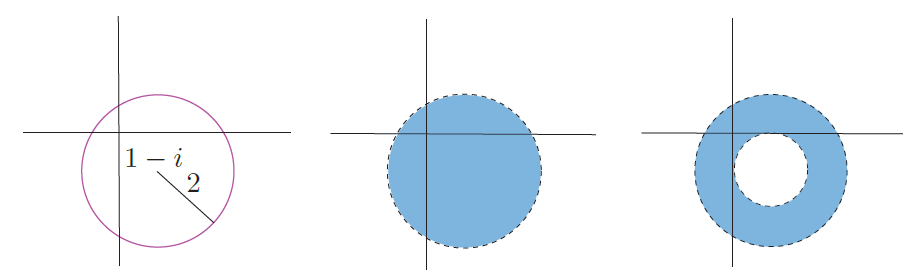
\includegraphics[width=0.8\textwidth]{./figs/fig-5-7}
\end{center}
\caption{왼쪽부터 $|z-(1-i)|=2$, $|z-(1-i)|<2$,
$1<|z-(1-i)|<2$}
\label{fig-5-7}
\end{figure}
\item[(4):] $z=x+iy$ ($x,y\in\mathbb R$)이라 하면,
$\Re(z-(1-i))=3$은 $x-1=3$과 동치이므로, $x=4$이다.
\begin{figure*}[h!]
\begin{center}
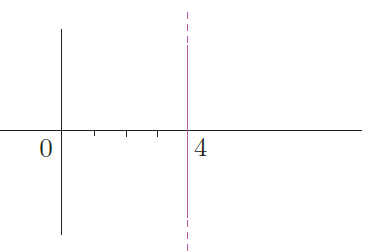
\includegraphics[width=0.3\textwidth]{./figs/fig-s-0-2}
\end{center}
%\caption{$RP$와 $SQ$는 길이가 같고 수직으로 만난다}
%\label{fig-5-5}
\end{figure*}
\item[(5):] $z=x+iy$ ($x,y\in\mathbb R$)이라 하면,
$|\Im(z-(1-i))|<3$은 $|y+1|<3$, 즉, $-4<y<2$와 같다.
\begin{figure*}[h!]
\begin{center}
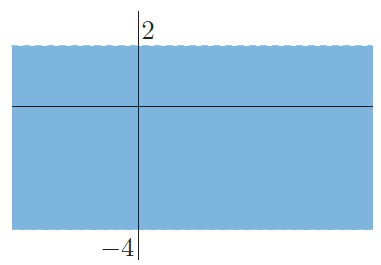
\includegraphics[width=0.3\textwidth]{./figs/fig-s-0-3}
\end{center}
%\caption{$RP$와 $SQ$는 길이가 같고 수직으로 만난다}
%\label{fig-5-5}
\end{figure*}
\item[(6):] $\{ z\in\mathbb C\,:\, |z-(1-i)| = |z-(1+i)|\}$는
$1-i$와 $1+i$에서 같은 거리에 있는 복소수 $z$의 집합이다.
따라서, $1-i$와 $1+i$을 잇는 선분의 수직이등분선이 된다.
즉, 실수축이다.
\begin{figure}[h!]
\begin{center}
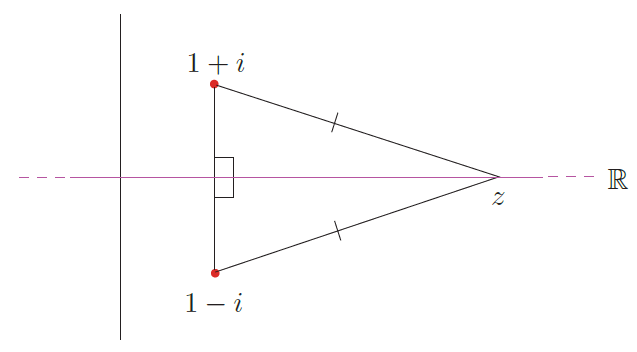
\includegraphics[width=0.6\textwidth]{./figs/fig-5-8}
\end{center}
\caption{$|z-(1-i)| = |z-(1+i)|$를 만족하는 집합은 $\mathbb R$}
\label{fig-5-8}
\end{figure}
\item[(7):] 방정식 $|z-(1-i)| + |z-(1+i)| =2$는 
$z$에서 $1+i$까지의  거리와  $1-i$까지의 거리의 합이 $2$가 됨을 의미한다.
그런데 $1-i$와 $1+i$의 거리가 $2$이므로
$z$는 $1-i$와 $1+i$를 잇는 선분에 있다.

직접 계산하는 방식으로도 같은 결과를 얻을 수 있다.
$z=x+iy$ ($x,y\in\mathbb R$)이면
\begin{align*}
2 &= \sqrt{(x-1)^2 + (y+1)^2} + \sqrt{(x-1)^2 + (y-1)^2} \\
&\ge |y+1| + |y-1| \ge 1 + \cancel{y} + 1 - \cancel{y} =2
\end{align*}
이므로 $|y+1| + |y-1|=2$이고, $x=1$이다.
\begin{figure}[h!]
\begin{center}
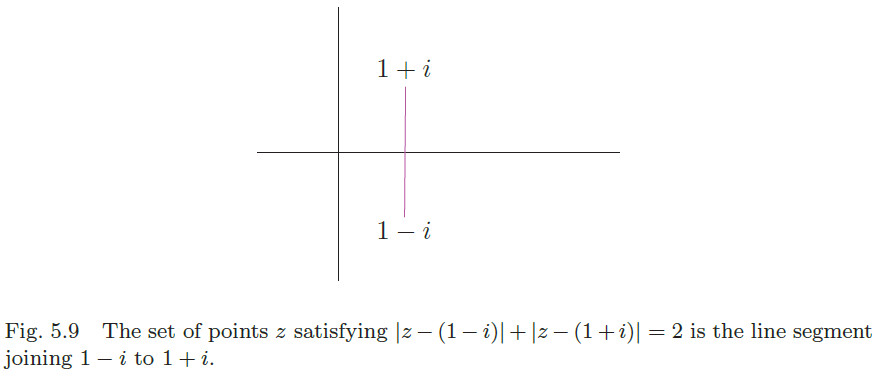
\includegraphics[width=0.6\textwidth]{./figs/fig-5-9}
\end{center}
\caption{$|z-(1-i)| + |z-(1+i)|=2$를 만족하는 집합은 $1-i$와 $1+i$를 잇는 선분이다.}
\label{fig-5-9}
\end{figure}
\item[(8):] 방정식 $|z-(1-i)| + |z-(1+i)| =3$을 만족하는 집합은
초점이 $1+i$와 $1-i$인 타원 $E$이 된다.
따라서, $\{z\in\mathbb C\,:\, |z-(1-i)| + |z-(1+i)| < 3\}$은
타원 $E$의 내부가 된다.
\begin{figure}[h!]
\begin{center}
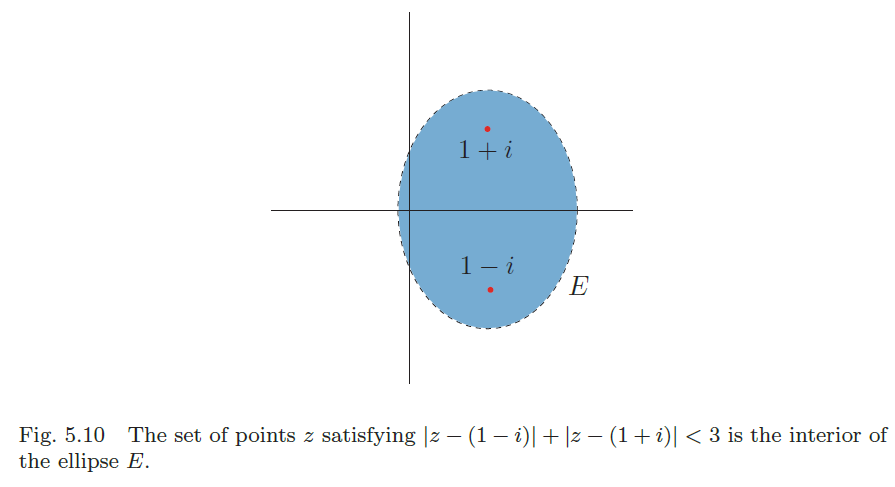
\includegraphics[width=0.6\textwidth]{./figs/fig-5-10}
\end{center}
\caption{$|z-(1-i)| + |z-(1+i)| < 3$을 만족하는 집합은 타원  $E$의 내부이다.}
\label{fig-5-10}
\end{figure}
\end{itemize}

\subsection*{연습문제 \ref{ex-1-24}}

$z\ne0$에 대하여
$p(z) = z^d \left( c_d + \dfrac{c_{d-1}}z + \cdots + \dfrac{c_1}{z^{d-1}}
+ \dfrac{c_0}{z^d} \right)$.
\[
\lim_{n\to\infty}  \left( 
 \dfrac{|c_{d-1}|}n + \cdots + \dfrac{|c_1|}{n^{d-1}}
+ \dfrac{|c_0|}{n^d} \right) = 0
\]
이므로, 
다음을  만족하도록 충분히 큰 $N$을 잡을 수 있다.
\[
\dfrac{|c_{d-1}|}N + \cdots + \dfrac{|c_1|}{N^{d-1}}
+ \dfrac{|c_0|}{N^d} < \dfrac{|c_d|}2.
\]
그러면 $|z|>N=:R$에 대하여
\begin{align*}
|p(z)| &= |z^d| \left|
c_d + \dfrac{c_{d-1}}z + \cdots + \dfrac{c_1}{z^{d-1}}
+ \dfrac{c_0}{z^d} \right| \\
&\ge |z|^d \left( |c_d| - \left| \dfrac{c_{d-1}}z + \cdots + \dfrac{c_1}{z^{d-1}}
+ \dfrac{c_0}{z^d} \right| \right) \\
&\ge |z|^d \left(|c_d| - \left( \dfrac{|c_{d-1}|}{|z|} + \cdots + \dfrac{|c_1|}{|z|^{d-1}}
+ \dfrac{|c_0|}{|z|^d} \right) \right) \\
&\ge |z|^d \left(|c_d| - \left( \dfrac{|c_{d-1}|}N + \cdots + \dfrac{|c_1|}{N^{d-1}}
+ \dfrac{|c_0|}{N^d} \right) \right) \\
&\ge |z|^d \left(|c_d| - \dfrac{|c_d|}2 \right) = \underbrace{\dfrac{|c_d|}2}_{=:M} |z|^d.
\end{align*}

\subsection*{연습문제 \ref{ex-1-25}}

$(\Leftarrow):$ 

실수열 $(\Re(z_n))_{n\in\mathbb N}$과 
$(\Im(z_n))_{n\in\mathbb N}$가 각각 $\Re(L)$과 $\Im(L)$로 수렴한다고 하자.
그러면, 주어진 $\epsilon>0$에 대하여,
충분히 큰 $N$이 존재하여 $n>N$이면
\[
|\Re(z_n) - \Re(L)| < \dfrac\epsilon{\sqrt{2}},\quad
|\Im(z_n) - \Im(L)| < \dfrac\epsilon{\sqrt{2}}
\]
을 만족하게 할 수 있고,
\begin{align*}
|z_n-L| &= \sqrt{ (\Re(z_n) - \Re(L))^2 + (\Im(z_n) - \Im(L))^2} \\
&< \sqrt{\left(\dfrac\epsilon{\sqrt{2}}\right)^2  + \left(\dfrac\epsilon{\sqrt{2}}\right)^2}
= \epsilon.
\end{align*}
따라서 $(z_n)_{n\in\mathbb N}$은 $L$로 수렴한다.

\noindent $(\Rightarrow):$

$(z_n)_{n\in\mathbb N}$이 $L$로 수렴한다고 가정하자.
$n>N$이면  $|z-L|<\epsilon$이 되도록 하는 $N$을 잡을 수 있다.
그러면 모든 $n>N$에 대하여,
\begin{align*}
|\Re(z_n) - \Re(L)| &= |\Re(z_n -L)| \le |z_n -L| <\epsilon, \\
|\Im(z_n) - \Re(L)| &= |\Im(z_n -L)| \le |z_n -L| <\epsilon
\end{align*}
이 되어
$(\Re(z_n))_{n\in\mathbb N}$과 
$(\Im(z_n))_{n\in\mathbb N}$이 각각 
$\Re(L)$과 $\Im(L)$로 수렴한다.

\subsection*{연습문제 \ref{ex-1-26}}

$(\Rightarrow):$

$(z_n)_{n\in\mathbb N}$이 $L$로 수렴한다고 가정하자.
그러면 $(\Re(z_n))_{n\in\mathbb N}$과 
$(\Im(z_n))_{n\in\mathbb N}$이 각각 
$\Re(L)$과 $\Im(L)$로 수렴한다.
따라서 $(\Re(z_n))_{n\in\mathbb N}$과 
$(-\Im(z_n))_{n\in\mathbb N}$은 각각 
$\Re(L)$과 $-\Im(L)$로 수렴한다.
즉, $(\Re(\overline{z_n}))_{n\in\mathbb N}$과 
$(\Im(\overline{z_n}))_{n\in\mathbb N}$이 각각 
$\Re(\overline{L})$과 $\Im(\overline{L})$로 수렴한다.
결론적으로 $(\overline{z_n})_{n\in\mathbb N}$이 $\overline{L}$로 수렴한다.

\noindent $(\Leftarrow):$ 

$(\overline{z_n})_{n\in\mathbb N}$이 $\overline{L}$로 수렴한다고 하자.
앞의 증명에서 $(\overline{(\overline{z_n})})_{n\in\mathbb N}$이 
$\overline{(\overline{L})}$로 수렴한다.
다시 쓰면, $(z_n)_{n\in\mathbb N}$이 $L$로 수렴한다.

\subsection*{연습문제 \ref{ex-1-27}}



%===[salt] 2장
% !TEX root = ./CA_solution.tex

\section*{2장 - 연습문제 풀이}

\subsection*{연습문제 \ref{ex-2-1}}

$z\ne0$에 대하여
\[
\dfrac{f(z) - f(0)}{z-0} - 0 = \dfrac{|z|^2-0}{z-0} = \dfrac{|z|^2}z.
\]
주어진 $\epsilon>0$에 대하여 $ \delta=\epsilon$으로 잡으면,
$0<|z-0|=|z| <\delta$일 때,
\[
\left| \dfrac{f(z) - f(0)}{z-0} - 0\right|
= \left| \dfrac{|z|^2}z \right|  = \dfrac{|z|^2}{|z|} = |z| < \delta = \epsilon.
\]
따라서 $f$는 $0$에서 복소미분가능하고 $f'(0)=0$이다.

\subsection*{연습문제 \ref{ex-2-2}}

$w_0\in \mathbb D^*$라 하자. 그러면 $\overline{w_0}\in D$이다.
$f$가 $D$에서 복소해석함수이므로, 주어진 $\epsilon>0$에 대응하는 
$\delta>0$가 존재하여,
$0<|z-\overline{w_0}| < \delta$이면 $z\in D$와
\begin{equation}\label{eq-5-17}
\left| \dfrac{f(z) - f(\overline{w_0})}{z-\overline{w_0}} - f'(\overline{w_0}) \right| < \epsilon
\end{equation}
를 만족한다.
이제 $w$를 $0<|w-w_0| <\delta$로 잡으면
\[
0< |w-w_0| = |\overline{w-w_0}| = |\overline{w} - \overline{w_0}| < \delta
\]
이 되어 $w\in D^*$이다.
또한,
\begin{align*}
\left| \dfrac{f^*(w) - f^*(w_0)}{w-w_0} - \overline{f'(\overline{w_0})} \right|
&= \left| \dfrac{\overline{f(\overline{w})} - \overline{f(\overline{w_0})}}{w-w_0} 
- \overline{f'(\overline{w_0})} \right| \\
&= \left| \overline{ \dfrac{f(\overline{w}) - f(\overline{w_0})}{w-w_0} 
- f'(\overline{w_0})} \right| \\
&= \left| \dfrac{f(\overline{w}) - f(\overline{w_0})}{w-w_0} 
- f'(\overline{w_0}) \right| < \epsilon \text{ \ (식 \eqref{eq-5-17}\을 이용하여)}
\end{align*}
이 되므로, $f^*$는 $w_0$에서 복소미분가능하며
$(f^*)'(w_0)= \overline{f'(\overline{w_0})}$이다.
$w_0\in D^*$를 임의로 선택할 수 있으므로
$f^*$는 $D^*$에서 복소미분가능함수이다.

\subsection*{연습문제 \ref{ex-2-3}}

$f$가 $z_0$에서 복소미분가능하므로,
상수 $r>0$과 함수 $h:D(z_0,r)\to \mathbb C$가 존재하여
$|z-z_0|<r$에 대하여
\[
f(z) = f(z_0) + (f'(z_0) + h(z))(z-z_0)
\]
로 쓸 수 있고
\[
\lim_{z\to z_0} h(z) = 0
\]
이다.
여기서, $D(z_0,r):= \{ z\in \mathbb C \,:\, |z-z_0| < r\} \subset D$이다.

$D(z_0,r'):= \{ z\in \mathbb C \,:\, |z-z_0| < r'\} \subset D(z_0,r) \subset D$과
$|h(z)|<1$이 되도록 $r'<r$을 잡자.
이제 주어진 $\epsilon>0$에 대하여
\[
\delta = \min\left\{ \dfrac\epsilon{|f'(z_0)|+1}, r' \right\}
\]
로 선택하면, $0<|z-z_0|<\delta$일 때, 
$z\in D(z_0, r')$이고,
\begin{align*}
|f(z) - f(z_0)| = |f'(z_0) + h(z)||z-z_0|
&\le ( |f'(z_0)|+|h(z)|)\dfrac{\epsilon}{ |f'(z_0)|+1} \\
&< ( |f'(z_0)|+1)  \dfrac{\epsilon}{|f'(z_0)|+1} = \epsilon.
\end{align*}
따라서 $f$는 $z_0$에서 연속이다.

\subsection*{연습문제 \ref{ex-2-4}}

$f,g:U\to \mathbb C$가 $z_0\in U$에서 복소미분가능함을 이용하면,
보조정리 \ref{lem-2-1}\로부터
$r>0$과 $h_f, h_g: D(z_0,r) \to \mathbb C$가 존재하여
(단, $D(z_0,r):= \{ z\in \mathbb C \,:\, |z-z_0| < r\}$)

$|z-z_0|<r$이면,
\begin{align}
f(z) & = f(z_0) + (f'(z_0) +h_f(z))(z-z_0), \label{eq-5-18} \\
g(z) & = g(z_0) + (g'(z_0) +h_g(z))(z-z_0), \label{eq-5-19}
\end{align}
와 $\Lim_{z\to z_0} h_f(z)  = 0 = \Lim_{z\to z_0} h_g(z)$를 만족한다.
\begin{itemize}
\item[(1)] 식 \eqref{eq-5-18}\과 \eqref{eq-5-19}\를 더하면,
$|z-z_0|<r$에 대하여
\[
(f+g)(z) = (f+g)(z_0) + \left( f'(z_0) + g'(z_0) + h_{f+g}(z) \right)(z-z_0)
\]
를 만족한다. 단, $D(z_0,r)$에서 $h_{f+g} (z) := h_f(z) + h_g(z)$로 정의한다.
또한,
\[
\lim_{z\to z_0} h_{f+g}(z) = \lim_{z\to z_0} ( h_f(z) + h_g(z) )
= \lim_{z\to z_0} h_f(z) + \lim_{z\to z_0} h_g(z) = 0+0 = 0.
\]
보조정리 \ref{lem-2-1}에 의하여
$f+g$는 복소미분가능하며 $(f+g)'(z_0) = f'(z_0) + g'(z_0)$이다.
\item[(2)] 식 \eqref{eq-5-18}에 $\alpha$를 곱하면,
$|z-z_0|<r$에 대하여
\[
(\alpha \cdot f)(z) = (\alpha \cdot f)(z_0) + \left(
\alpha\cdot f'(z_0) + h_{\alpha\cdot f}(z) \right) (z-z_0),
\]
단, $D(z_0,r)$에서 $h_{\alpha\cdot f}(z) := \alpha \cdot f(z)$이다.
또한,
\[
\lim_{z\to z_0} h_{\alpha\cdot f}(z) = \lim_{z\to z_0} (\alpha\cdot h_f(z))
= \alpha \cdot \lim_{z\to z_0} h_f(z) = \alpha\cdot 0 = 0.
\]
보조정리 \ref{lem-2-1}에 의하여
$\alpha \cdot f$는 복소미분가능하며 $(\alpha\cdot f)'(z_0) =\alpha\cdot f'(z_0)$이다.

\item[(3)] 식 \eqref{eq-5-18}\과 \eqref{eq-5-19}\를 곱하면,
$|z-z_0|<r$에 대하여
\[
(fg)(z) = (fg)(z_0) + \left( f'(z_0)g(z_0) + f(z_0)g'(z_0) + h_{fg}(z) \right) (z-z_0),
\]
단, $D(z_0,r)$에서
\[
h_{fg}(z):= f(z_0)h_g(z) + g(z_0)h_f(z) + (z-z_0)(f'(z_0)+h_f(z))(g'(z_0)+h_g(z))
\]
또한,
\[
\lim_{z\to z_0} h_{fg}(z) = f(z_0)\cdot0 + g(z_0)\cdot 0 
+ 0\cdot (f'(z_0)+0)\cdot(g'(z_0)+0)=0
\]
이므로 $fg$는 $z_0$에서 복소미분가능하며
\[
(fg)'(z) = f'(z_0)g(z_0) + f(z_0)g'(z_0).
\]
\end{itemize}

\subsection*{연습문제 \ref{ex-2-5}}

$\Hol(\mathbb D)$가 $d$차의 유한차원이라고 하자.
그러면 $d+1$개의 벡터 $1,z, z^2, \ldots, z^d\in \Hol(\mathbb  D)$는
일차종속이다. 따라서 모두 $0$은 아닌 $\alpha_0, \ldots, \alpha_d$가 존재하여
\[
\alpha_0\cdot 1 + \alpha_1\cdot z + \cdots + \alpha_d \cdot z^d = 0
\quad(z\in \mathbb D)
\]
을 만족한다.
$k\in \{0, 1, \ldots, d\}$를 $\alpha_k \ne 0$인 가장 작은 값이라 하자.
그러면, $k$번 미분한 값을 $0\in \mathbb D$에서 계산하면
\[
0 + \alpha_k \cdot k! + 0 = 0
\]
이므로 $\alpha_k=0$이 되어 모순이다.

\subsection*{연습문제 \ref{ex-2-6}}

$z_0\in U$라 하자. $f$는 $z_0$에서 복소미분가능하므로
$r>0$과 $D(z_0,r) := \{ z\in \mathbb C\,:\, |z-z_0|<r\} \subset U$에 정의된
복소함수 $h$가 존재하여
\[
f(z) = f(z_0) + (f'(z_0) +h(z))(z-z_0),
\quad z\in D(z_0,r)
\]
과
\begin{equation}\label{eq-5-20}
\lim_{z\to z_0} h(z)=0
\end{equation}
을 만족한다.
$g:=1/f$라 하면,
\[
\dfrac1{g(z)} = \dfrac1{g(z_0)} + (f'(z_0) +h(z))(z-z_0)
\]
이므로 $g(z_0) = g(z) + (f'(z_0)+h(z))g(z_0)g(z)\cdot(z-z_0)$.
정리하면
\begin{align*}
g(z) &= g(z_0) + (-f'(z_0)g(z_0)g(z) - h(z)g(z_0)g(z)))\cdot(z-z_0) \\
&= g(z_0) + \left( - \dfrac{f'(z_0)}{(f(z_0))^2} + \dfrac{f'(z_0)}{(f(z_0))^2}
- \dfrac{f'(z_0)}{f(z_0)f(z)} - \dfrac{h(z)}{f(z_0)f(z)} \right) (z-z_0) \\
&= g(z_0) + \left( - \dfrac{f'(z_0)}{(f(z_0))^2} + \varphi(z) \right)\cdot(z-z_0),
\end{align*}
$z\in D(z_0,r)$에서
\[
\varphi(z):= \dfrac{f'(z_0)}{(f(z_0))^2}
- \dfrac{f'(z_0)}{f(z_0)f(z)} - \dfrac{h(z)}{f(z_0)f(z)}.
\]
$z_0$에서 $f$의 연속성과 식 \eqref{eq-5-20}\로부터
\[
\lim_{z\to z_0} \varphi(z) = \cancel{\dfrac{f'(z_0)}{(f(z_0))^2}}
- \cancel{\dfrac{f'(z_0)}{f(z_0)f(z_0)}} - \dfrac{0}{f(z_0)f(z_0)} = 0.
\]
따라서 $g$가 $z_0$에서 복소미분가능하며
\[
g'(z_0) = - \dfrac{f'(z_0)}{(f(z_0))^2}.
\]

\subsection*{연습문제 \ref{ex-2-7}}

$m\ge0$인 경우는 이미 증명했으므로, 
$m= -n$ ($n\in \mathbb N$)인 경우를 생각하자.
$f(z):=z^n$ ($z\in \mathbb C\setminus \{0\}$)에  대하여 함수
\[
z\mapsto z^m = z^{-n} = \dfrac1{z^n} = \dfrac1{f(z)}
\]
는 복소해석함수이고 $\mathbb C\setminus \{0\}$에서 함수값이
$0$은 아니므로
$1/f$도 복소해석함수이고, 미분은
\[
\left(\dfrac1f\right)'(z) = - \dfrac{f'(z)}{(f(z))^2} = - \dfrac{nz^{n-1}}{(z^n)^2}
= -n \dfrac1{z^{n+1}} = m \cdot \dfrac1{z^{-m+1}} = mz^{m-1}
\]
이 되어 증명이 끝난다.

\subsection*{연습문제 \ref{ex-2-8}}

$f: \mathbb D \to \mathbb C$를 
\[
f(z) = -\dfrac{1+z}{1-z},\quad z\in \mathbb D
\]
로 정의하고, $f: \mathbb C \to \mathbb C$를 $g(z)= \exp z$로 정의하자.
그러면, $f(\mathbb D) \subset \mathbb C = D_g$.
따라서 $g\circ f$는 $\mathbb D$에서 복소해석함수이고,
\begin{align*}
(g\circ g)'(z) &= g'(f(z))\cdot f'(z) 
= \exp\left( - \dfrac{1+z}{1-z}\right) \cdot \dfrac d{dz}\left( - \dfrac{1+z}{1-z}\right) \\
&= \exp\left( - \dfrac{1+z}{1-z}\right)\cdot \left(
-(1+z)\dfrac d{dz} \left(\dfrac1{1-z}\right) - \dfrac1{1-z}\dfrac d {dz}(1+z)\right) \\
&= \exp\left( - \dfrac{1+z}{1-z}\right) \cdot \left(
-\dfrac{1+z}{(1-z)^2} - \dfrac1{1-z} \right) \\
&= - \dfrac2{(1-z)^2} \exp\left( - \dfrac{1+z}{1-z}\right).
\end{align*}
따라서, $z\in\mathbb D$에 대하여,
$\dfrac d{dz} \left( \exp\left( - \dfrac{1+z}{1-z}\right) \right)
=  - \dfrac2{(1-z)^2} \exp\left( - \dfrac{1+z}{1-z}\right)$.

\subsection*{연습문제 \ref{ex-2-9}}

$z = x+iy$ ($x,y\in\mathbb R$)라 하면,
$|z|^2 = x^2+y^2$.
따라서, $u, v$를 각각 $|z|^2$의 실수부와 허수부라 하면,
$u=x^2+y^2$, $v=0$이다. 따라서,
\begin{align*}
\dfrac{\partial u}{\partial x} &=2x, \quad \dfrac{\partial v}{\partial y} = 0, \\
\dfrac{\partial u}{\partial y} &=2y, \quad \dfrac{\partial v}{\partial x} = 0.
\end{align*}
$z\ne0$이므로, $x$ 또는 $y$중 하나는 $0$이 아니다.
즉, 코시-리만 방정식 중 적어도 하나는 만족되지 않는다.
\begin{align*}
\left( \dfrac{\partial u}{\partial x} = \right) 2x &\ne 0 
\left( = \dfrac{\partial v}{\partial y} \right) \text{ 또는} \\
\left( \dfrac{\partial u}{\partial y} = \right) 2y &\ne 0 
\left( = - \dfrac{\partial v}{\partial x} \right).
\end{align*}
결론적으로 $|z|^2$은 $0$이 아닌 점에서 미분이 불가능하다.

\subsection*{연습문제 \ref{ex-2-10}}

$z = x+iy$ ($x,y\in\mathbb R$)라 하면,
\begin{align*}
z^3 &= (x+iy)^3 = x^3 + 3x^2(iy) + 3x(iy)^2 + (iy)^3 \\
&= x^3 - 3xy^2 + i(3x^2y-y^3).
\end{align*}

$u$, $v$를 각각 $z^3$의 실수부와 허수부라 하면,
\begin{align*}
u(x,y) &= x^3 -3xy^2, \\
v(x,y) &= 3x^2y - y^3.
\end{align*}

$u$, $v$는 연속미분가능하고 (즉, $u,v\in C^1$)
\begin{align*}
\dfrac{\partial u}{\partial x} &= 3x^2 -2y^2 = \dfrac{\partial v}{\partial y} \text{ 이고}, \\
\dfrac{\partial u}{\partial y} &= -6xy = - \dfrac{\partial v}{\partial x}.
\end{align*}
즉, $\mathbb R^2$의 모든 점에서 코시-리만 방정식을 만족하므로,
$z\mapsto z^3$은 전해석함수이다.

\subsection*{연습문제 \ref{ex-2-11}}

$z = x+iy$ ($x,y\in\mathbb R$)라 하면,
$\Re(z) = \Re(x+iy) = x$.
따라서, $u, v$를 각각 $\Re(z)$의 실수부와 허수부라 하면,
\begin{align*}
u & =x, \\
v &=0.
\end{align*}
따라서, 모든 $(x,y) \in \mathbb R^2$에서
\[
\dfrac{\partial u}{\partial x}  = 1 \ne 0 =  \dfrac{\partial v}{\partial y}.
\]
즉, 코시-리만 방정식은 $\mathbb R^2$의 어떤 점에서도 만족되지 않는다.
결론적으로 $\mathbb C$의 모든 점에서 $\Re(z)$는 복소미분가능하지 않다.

\subsection*{연습문제 \ref{ex-2-12}}

$u$, $v$를 각각 $f$의 실수부와 허수부라 하자. 
그러면, $v=0$이고,
\[
\dfrac{\partial u}{\partial x} = \dfrac{\partial v}{\partial y} = 0
\text{ 이고 }
\dfrac{\partial u}{\partial y} = - \dfrac{\partial v}{\partial x} = 0.
\]
따라서 
\[
u(x,y_0) = u(x_0,y_0) = \int_{x_0}^z \dfrac{\partial u}{\partial y}(\xi, y_0) d\xi = 0
\]







%




%===[salt] 3장
% !TEX root = ./CA_solution.tex

\section*{3장 - 연습문제 풀이}

\subsection*{연습문제 \ref{ex-3-1}}

$\gamma_1 = \cos t + i\sin t$, $\gamma_2 = \cos (2t) + i\sin (2t)$,
$\gamma_3 = \cos t - i\sin t$이므로
$k=1,2,3$ 각각의 경우 모두 $(\Re(\gamma_k(t)))^2 + (\Im(\gamma_k(t)))^2=1$이다.
$\gamma_k$의 상은 중심이 $0$이고 반지름이 $1$인 원 $\mathbb T$에 있다.
$\theta \in [0,2\pi)$에 대하여 $z = \exp(i\theta)$이면,
$z = \gamma_1(\theta) = \gamma_2(\theta/2) = \gamma_3(2\pi - \theta)$이다.
따라서 $\mathbb T$위의 모든 점은 $\gamma_1, \gamma_2, \gamma_3$ 각각에 의한 상에
속한다.
\begin{align*}
\int_{\gamma_1} \dfrac1z dz &= \int_0^{2\pi} \dfrac1{\exp(it)}\cdot i\exp(it)dt = 2\pi i, \\
\int_{\gamma_2} \dfrac1z dz &= \int_0^{2\pi} \dfrac1{\exp(2it)}\cdot 2i\exp(2it)dt = 4\pi i, \\
\int_{\gamma_3} \dfrac1z dz &= \int_0^{2\pi} \dfrac1{\exp(-it)}\cdot (-i)\exp(-it)dt = -2\pi i.
\end{align*}

\subsection*{연습문제 \ref{ex-3-2}}

실함수 $x,y$에 대하여 $\gamma(t) = x(t) +iy(t)$, $t\in[0,1]$라 하자.
또한, $u,v$를 각각 함수 $f$의 실수부와 허수부라 하면,
\begin{align*}
f'(\gamma(t))\cdot\gamma'(t)
&= \left( \dfrac{\partial u}{\partial x}(x(t),y(t)) +
i \dfrac{\partial v}{\partial x}(x(t),y(t)) \right) (x'(t) + iy'(t)) \\
&= \dfrac{\partial u}{\partial x}(x(t),y(t)) \cdot x'(t) - \dfrac{\partial v}{\partial x}y'(t) \\
&\qquad +i\left( \dfrac{\partial u}{\partial x}(x(t),y(t)) \cdot y'(t) + \dfrac{\partial v}{\partial x}x'(t) \right) \\
&= \dfrac{\partial u}{\partial x}(x(t),y(t)) \cdot x'(t) + \dfrac{\partial u}{\partial y}y'(t) \\
&\qquad +i\left( \dfrac{\partial v}{\partial y}(x(t),y(t)) \cdot y'(t) + \dfrac{\partial v}{\partial x}x'(t) \right) \\
&\qquad\qquad \text{(코시-리만 방정식을 적용함)} \\
&= \dfrac d{dt} u(x(t), y(t)) + i \dfrac d{dt} v(x(t),y(t)) \quad\text{(연쇄법칙을 적용함)} \\
&= \dfrac d{dt} (u(x(t), y(t)) + i v(x(t),y(t))) = \dfrac d{dt} f(\gamma(t)).
\end{align*}

\subsection*{연습문제 \ref{ex-3-3}}

원형경로 $\gamma$를 $\gamma(t) = 2\exp(it)$, $t\in[0,2\pi]$라 하자.
\begin{itemize}
\item[(1)] 
\begin{align*}
\int_\gamma (z+\bar z) dz & = \int_0^{2\pi} (2\exp(it) + 2\exp(-it))\cdot 2i \cdot \exp(it) dt \\
&= 4i\int_0^{2\pi} (\exp(2it) +1)dt - 4i\cdot 0 + 4i\cdot 2\pi = 8\pi i.
\end{align*}
\item[(2)] 
\begin{align*}
\int_\gamma (z^2-2z+3) dz & = \int_0^{2\pi} (4\exp(2it) - 4\exp(it)+3)\cdot 2i \cdot \exp(it) dt \\
&= \int_0^{2\pi} i(8\exp(3it) - 8\exp(2it) + 6\exp(it))dt  = 0+0+0 =0.
\end{align*}
\item[(3)] 
\begin{align*}
\int_\gamma xy dz & = \int_0^{2\pi}  2\cos t\cdot 2\sin t \cdot 2i \cdot(\cos t +i\sin t) dt \\
&= 4i\int_0^{2\pi} (\sin (2t))(\cos t + i\sin t)dt \\
&= 4i\int_{-\pi}^\pi \underbrace{(\sin(2t))\cos t}_{\text{기함수}} dt
- 2\int_0^{2\pi} (\cos t - \cos(3t))dt \\
&=0 - 2(0-0) = 0.
\end{align*}
\end{itemize}

\subsection*{연습문제 \ref{ex-3-4}}

\begin{itemize}
\item[(1)] $\gamma(t) =(1+i)t$, $t\in[0,1]$이므로,
$\dint_\gamma \Re(z)dz = \dint_0^1 t(1+i)dt = \dfrac{1+i}2$. 
\item[(2)] $\gamma(t) =1+\exp(it)$, $t\in[-\pi/2,0]$이므로, 
\begin{align*}
\int_\gamma \Re(z) dz &= \int_{-\pi/2}^0 (\cos t)i\exp(it)dt
= \int_{-\pi/2}^0 i(\cos t)^2 -(\cos t)(\sin t)dt \\
&= \int_{-\pi/2}^0 \left( i\dfrac{\cos(2t)+1}2 - \dfrac{\sin(2t)}2 \right) dt \\
&= 0 + i\cdot \dfrac12 \cdot \dfrac \pi2 + \dfrac12 = \dfrac12 + i\dfrac\pi4.
\end{align*}
\item[(3)] $\gamma(t) =t+it^ 2$, $t\in[0,1]$이므로,
\[
\int_\gamma \Re(z) dz  = \int_0^1 t\cdot(1+2it)dt = \dfrac12 + 2i\cdot\dfrac13 
=\dfrac12 + \dfrac23i.
\]
\end{itemize}

\subsection*{연습문제 \ref{ex-3-5}}

이항정리에 의하여
\[
(1+z)^n = \sum_{\ell = 0}^n  {n \choose \ell} z^\ell 1^{n-\ell} 
\sum_{\ell = 0}^n  {n \choose \ell} z^\ell.
\]
$0\le k \le n$에 대하여,
\[
\dfrac{(1+z)^n}{z^{k+1}} =\sum_{\ell = 0}^n  {n \choose \ell} z^{\ell-k-1}
\]
이므로
\begin{align*}
\dfrac1{2\pi i} \int_C \dfrac{(1+z)^n}{z^{k+1}}dz
&= \dfrac1{2\pi i} \int_C \sum_{\ell = 0}^n  {n \choose \ell} z^{\ell-k-1} dz \\
&  \sum_{\ell = 0}^n  {n \choose \ell} \dfrac1{2\pi i} \int_C  z^{\ell-k-1}dz
= {n \choose k}.
\end{align*}

\subsection*{연습문제 \ref{ex-3-6}}
\begin{itemize}
\item[(1)]
$U_f, V_f, U_g, V_g:[a,b] \to \mathbb R$에 대하여
$f(\gamma(t))\gamma'(t) = U_f(t) + iV_f(t)$,
$g(\gamma(t))\gamma'(t) = U_g(t) + iV_g(t)$, $t\in[a,b]$라고 하자.

\begin{align*}
\int_\gamma (f+g)(z)dz
&= \int_a^b (f+g)(\gamma(t))\cdot \gamma'(t)dt \\
&= \int_a^b \left( f(\gamma(t))\cdot \gamma'(t) + g(\gamma(t))\cdot \gamma'(t) \right) dt\\
&= \int_a^b (U_f(t) + U_g(t)) dt + i \int_a^b (V_f(t) + V_g(t)) dt \\
&= \int_a^b U_f(t)dt + \int_a^b V_f(t)dt + i\int_a^b V_f(t)dt + i\int_a^b V_g(t)dt \\
&= \int_\gamma f(z)dz + \int_\gamma g(z)dz.
\end{align*}

\item[(2)] $\alpha = p+iq$ ($p,q\in\mathbb R$)이고
$U,V:  [a,b] \to \mathbb R$에 대하여
$f(\gamma(t))\gamma'(t)  = U(t) + iV(t)$, $t\in[a,b]$라 하자.
그러면,
\begin{align*}
\int_\gamma (\alpha\cdot f)(z) dz
&= \int_a^b (p+iq)(U(t) + iV(t))dt \\
&= \int_a^b(pU(t) - qV(t))dt + i\int_a^b (pV(t) + qU(t))dt \\
&= p \left(\int_a^b U(t)dt + i \int_a^b V(t)dt \right)
+ iq\left(\int_a^b U(t)dt + i \int_a^b V(t)dt \right) \\
&= (p+iq)\left(\int_a^b U(t)dt + i \int_a^b V(t)dt \right)
= \alpha \cdot \int_\gamma f(z)dz.
\end{align*}
\end{itemize}

\subsection*{연습문제 \ref{ex-3-7}}

$-(-\gamma): [a,b] \to \mathbb C$는 다음 식으로 주어진다.
\[
(-(-\gamma))(t)= (-\gamma)(a+b-t) = \gamma(a+b-(a+b-t)) = \gamma(t),
\quad t\in[a,b].
\]
따라서 $-(-\gamma) = \gamma$이며, 그림으로 보면 직관적으로 명백하다.

\subsection*{연습문제 \ref{ex-3-8}}

$\gamma(b) = (-\gamma)(a)$이므로
$\gamma$와 $-\gamma$는 결합가능한 경로이다.
\[
\int_{\gamma+(-\gamma)} f(z) dz = \int_\gamma f(z) dz + \int_{-\gamma} f(z)dz
=  \int_\gamma f(z) dz - \int_\gamma f(z) dz = 0.
\]

\subsection*{연습문제 \ref{ex-3-9}}

$\gamma:[0,1] \to \mathbb C$를 $\gamma(t) = (1+i)t$, $t\in [0,1]$이라 하자.
피타고라스 정리를 쓰면, $\gamma$의 길이는 $\sqrt{1^2+1^2} = \sqrt{2}$.

\begin{figure*}[h!]
\begin{center}
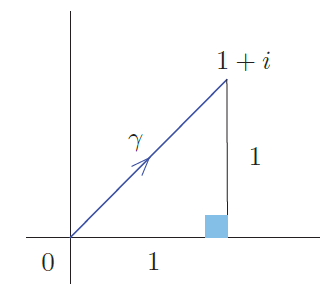
\includegraphics[width=0.3\textwidth]{./figs/fig-s-0-8}
\end{center}
%\caption{$\left\{ z \in\mathbb C \,:\, z\ne0, \dfrac\pi4 < |\Arg(z)| < \dfrac\pi3 \right\}$}
%\label{fig-5-14}
\end{figure*}

또한 $|(\gamma(t))^2| = |t+it|^2 = 2t^2$이고,
$\max\limits_{t\in[0,1]} |(\gamma(t))^2| = 2\cdot 1^2 = 2$.
따라서
\[
\left| \int_\gamma z^2dz \right|
\le \left( \max\limits_{t\in[0,1]} |(\gamma(t))^2|  \right) \cdot
(\text{$\gamma$의 길이})
= 2\sqrt{2}.
\]
직접 계산하면,
\begin{align*}
\int_\gamma z^2 dz = \int_0^1 (t+it)^2\cdot(1+i)dt
= \int_0^1 (1+i)^3t^2dt = \dfrac{(1+i)^3}3
\end{align*}
이므로
$\left| \dint_\gamma z^2 dz \right| = \dfrac{(\sqrt{3})^3}3 = \dfrac{2\sqrt{2}}3$.

\subsection*{연습문제 \ref{ex-3-10}}

\begin{align*}
{2n \choose n} = \left|  {2n \choose n} \right|
&= \left| \dfrac1{2\pi i}\int_C \dfrac{(1+z)^{2n}}{z^{n+1}}dz \right| \\
&\le \dfrac1{2\pi} \left( \max_{|z|=1} \left| \dfrac{(1+z)^{2n}}{z^{n+1}}\right| \right)
\cdot 2\pi\cdot 1 = \max_{|z|=1} \dfrac{|1+z|^{2n}}1 \\
&\le (1+1)^{2n} = 2^{2n} = 4^n.
\end{align*}

\subsection*{연습문제 \ref{ex-3-11}}

$F=U+iV$를 $\bar z \in \mathbb C$의 부정적분이라고 하자.
그러면,
\[
\dfrac{\partial U}{\partial x}  + i \dfrac{\partial V}{\partial x}
= \dfrac{\partial V}{\partial y} - i\dfrac{\partial U}{\partial y}
= F' = \bar z = x-iy.
\]

$x_0\in\mathbb R$을 고정하자. 그러면 $(x,y)\in\mathbb R^2$에 대하여
\[
V(x,y ) - V(x_0, y) = \int_{x_0}^x \dfrac{\partial V}{\partial x}(\xi, y )d\xi
= \int_{x_0}^x -y d\xi = -xy +x_0y.
\]
따라서 $V(x,y) = -xy + \varphi(y)$, $\varphi(y):+V(x_0,y_0) + x_0y$이면,
\[
x  = \dfrac{\partial V}{\partial y} = -x + \varphi'(y).
\]
즉, 모든 $x\in\mathbb R$에 대하여 $\varphi'(y) = 2x$인데
이는 분명 모순이다.
특히, $2\cdot 1 = 2 = \varphi'(y) = 2\cdot  0 = 0$.

\subsection*{연습문제 \ref{ex-3-12}}

$(fg)' = fg' + f'g$이므로
함수 $\zeta \mapsto f(\zeta)g'(\zeta) + f'(\zeta)g(\zeta)$는 
부정적분을 갖는다.
따라서 경로적분의 기본정리에 의하여
\[
\int_\gamma \left( f(\zeta)g'(\zeta) + f'(\zeta)g(\zeta) \right) d\zeta
= f(z)g(z) - f(w)g(w)
\]
이고 이를 정리하면 원하는 결과를 얻는다.

\subsection*{연습문제 \ref{ex-3-13}}

$\mathbb C$에서 $\sin' z = \cos z$이므로 $\cos z$는 부정적분을 갖는다.
따라서 경로적분의 기본정리에 의하여
\begin{align*}
\int_\gamma \cos z \, dz 
&= \sin i - \sin (-i) = 2\sin i = 2\dfrac{\exp(i\cdot i) - \exp(-i\cdot i)}{2i}
= \dfrac{e^{-1} - e^{1}}i \\
&= \left( e - \dfrac1e \right)i.
\end{align*}


\subsection*{연습문제 \ref{ex-3-14}}

$\mathbb C$에서  $\exp' z = \exp z$이므로
$0$과 $a+ib$를 잇는 경로 $\gamma$를 따라 적분하면
\[
\int_\gamma \exp z\, dz = \exp(a+ib) - \exp 0 = e^a(\cos b + i \sin b) -1
= e^a\cos b -1 +ie^a\sin b.
\]
 경로를 $\gamma(x) = (a+ib)x$, $x\in[0,1]$로 잡으면,
\[
\int_\gamma \exp z\, dz = \int_0^1 \exp(a+ib)\cdot (a+ib)dx
= \int_0^1 e^{ax}(\cos(bx) + i\sin(bx))(a+ib)dx.
\]
 따라서,
$(a-ib)\dint_\gamma \exp z\, dz = \dint_0^1 e^{ax}(\cos(bx) + i\sin(bx))(a^2+b^2)dx$이고,
\begin{align*}
(a^2+b^2) \int_0^1 e^{ax} \cos (bx)dx
&= \Re\left( (a-ib)\int_\gamma \exp z\, dz \right) \\
&= \Re((a-ib)(e^a\cos b -1 + ie^a\sin b)) \\
&= a(e^a\cos b -1) + be^a \sin b.
\end{align*}
즉,
$\dint_0^1 e^{ax}\cos(bx)\, dx = \dfrac{a(e^a\cos b - 1) + be^a\sin b}{a^2+b^2}$.

\subsection*{연습문제 \ref{ex-3-15}}

중심이 $0$이고 반지름 $r>0$인 원을 반시계방향으로 도는 닫힌경로 $C$를 생각하자.
$C(\theta) = r\exp(i\theta)$, $\theta\in[0,2\pi]$.
경로적분의 기본정레에 의해
\begin{align*}
0 & = \int_C \exp z \, dz = \int_0^{2\pi} e^{r\cos\theta +ir\sin\theta}
\cdot ri\exp(i\theta)d\theta\\
&= \int_0^{2\pi} e^{r\cos\theta} \cdot r\cdot i \exp(i(r\sin\theta +\theta))d\theta.
\end{align*}
위 식에서 실수부만 취하면
\[
\int_0^{2\pi} e^{r\cos\theta} \cos(r\sin \theta + \theta)d\theta = 0.
\]

\subsection*{연습문제 \ref{ex-3-16}}

$\mathbb C\setminus\{0\}$에서 복소미분가능한 $F$가 $F'=1/z$를 만족한다고 하자.
중심이 $0$이고 반시계방향으로 도는 원형경로 $C$를 생각하자.
$C$가 닫힌경로 이므로, 경로적분의 기본정리에 의해
\[
\int_C F'(z)dz = 0.
\]
한편, 이미 알고있는 계산 결과에 따르면,
\[
\int_C F'(z)dz = \int_C \dfrac1z dz = 2\pi i
\]
이므로 모순이다.

\subsection*{연습문제 \ref{ex-3-17}}

(ER1)
$\gamma: [0,1] \to D$가 닫힌경로라고 하자.
$H:[0,1]\times[0,1] \to D$를 $H(t,s) = \gamma(t)$, $t,s\in[0,1]$로 정의하면,
$H$는 연속이고,
\begin{align*}
H(t,0) &=\gamma(t), \quad t\in[0,1],\\
H(t,1) &=\gamma(t), \quad t\in[0,1],\\
H(0,s) &=\gamma(0) = \gamma(1) = H(1,s), \quad s\in[0,1].
\end{align*}
따라서 $\gamma$는 자기자신과 $D$-호모토픽하다.
즉, 관계는 반사적(reflexive)이다.
(ER2)
$\gamma_0, \gamma_1: [0,1] \to D$가 닫힌경로이고
$\gamma_0$가 $\gamma_1$과 $D$-호모토픽하다고 하자.
그러면, 다음을 만족하는 연속함수 $H:[0,1]\times[0,1] \to D$가 존재한다.
\begin{align*}
H(t,0) &= \gamma_0(t), \quad t\in [0,1], \\
H(t,1) &= \gamma_1(t), \quad t\in [0,1], \\
H(0,s) &= H(1,s), \quad s\in [0,1].
\end{align*}
$\tilde H:[0,1]\times [0,1] \to D$를
$\tilde H(t,s) = H(t,-s)$, $t,s\in[0,1]$로 정의하자.
그러면, $\tilde H$는 연속이고 다음을 만족한다.
\begin{align*}
\tilde H(t,0) & = H(t,1) = \gamma_1(t), \quad t\in[0,1], \\
\tilde H(t,1) & = H(t,0) = \gamma_0(t), \quad t\in[0,1], \\
\tilde H(0,s) & = H(0,1-s) = H(1,1-s) = \tilde H(1,s), \quad s\in[0,1].
\end{align*}
따라서 $\gamma_1$은 $\gamma_0$와 $D$-호모토픽하다.
즉, 관계는 대칭적(symmetric)이다.

(ER3)
$\gamma_0, \gamma_1, \gamma_2$가 닫힌경로이고
$\gamma_0$가 $\gamma_1$과 $D$-호모토픽하고,
$\gamma_1$이 $\gamma_2$와 $D$-호모토픽하다고 하자.
그러면, 다음을 만족하는 연속함수  $H, K:[0,1]\times[0,1]\to D$가 존재한다.
\begin{align*}
H(t,0) = \gamma_0(t), \ t\in[0,1], \quad & K(t,0) = \gamma_1(t), \ t\in[0,1], \\
H(t,1) = \gamma_1(t), \ t\in[0,1], \quad & K(t,1) = \gamma_2(t), \ t\in[0,1], \\
H(0,s) = H(1,s), \ s\in[0,1], \quad & K(0,s) = K(1,s), \ s\in[0,1].
\end{align*}
$L:[0,1]\times[0,1]\to D$를
\[
L(t,s) = \begin{cases}
H(t,2s), & s\in [0, \frac12], \\
K\left(t, 2(s-\frac12)\right), & s\in (\frac12,1]
\end{cases}
\]
로 정의하면,
\begin{align*}
L(t,0) &= H(t,0) = \gamma_0(t), \quad t\in[0,1],\\
L(t,1) &= K(t,1) = \gamma_2(t), \quad t\in[0,1].
\end{align*}
또한, $0\le s\le \frac12$에 대하여 $L(0,s) = H(0,2s) = H(1,2s) = L(1,s)$, 
$\frac12 <s\le1$에 대하여
\[
L(0,s) = K\left( 0, 2(s - \frac12) \right) = K\left( 1, 2(s - \frac12) \right) = L(1,s).
\]
이다.

$[0,1]\times (\frac12,1]$에서 정의된 수열 $((t_n, s_n))_{n\in\mathbb N}$이
$(t_0,\frac12)$에 수렴한다면,
\begin{align*}
\lim_{n\to\infty} L(t_n, s_n)
& = \lim_{n\to\infty} K\left( t_n, 2(s_n - \frac12)\right)
= K(t_0,0) = \gamma_1(t_0) \\
&= H(t_0,1) = L\left( t_0, \frac12\right) = L\left( \lim_{n\to\infty} (t_n, s_n) \right).
\end{align*}
따라서 $L$은 연속함수이다.
결론적으로, $\gamma_0$는 $\gamma_2$와 $D$-호모토픽하다.
즉, 관계는 추이적(transitive)이다.

이상에서 $D$-호모토피 관계는 반사적, 대칭적, 추이적인 성질을 만족하므로
동치(equivalence) 관계이다.

\subsection*{연습문제 \ref{ex-3-18}}

그림에서 경로 $C$는 경로 $S$와 $\mathbb C\setminus \{0\}$-호모토픽함을 알 수 있다.

\begin{figure*}[h!]
\begin{center}
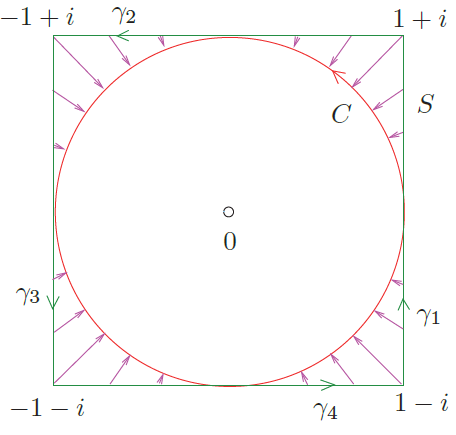
\includegraphics[width=0.4\textwidth]{./figs/fig-s-0-9}
\end{center}
%\caption{$\left\{ z \in\mathbb C \,:\, z\ne0, \dfrac\pi4 < |\Arg(z)| < \dfrac\pi3 \right\}$}
%\label{fig-5-14}
\end{figure*}

직접 계산을 위해 $t\in[0,1]$에 대하여 경로를 다음과 같이 정의하자.
\begin{align*}
\gamma_1(t) &:= (1-t)(1-i) + t(1+i) = 1 + i(2t-1), \\
\gamma_2(t) &:= (1-t)(1+i) + t(-1+i) = (1-2t) + i, \\
\gamma_3(t) &:= (1-t)(-1+i) + t(-1-i) = -1 + i(1-2t), \\
\gamma_4(t) &:= (1-t)(-1-i) + t(1-i) = 2t-1 -i.
\end{align*}
그러면,
\[
\int_S \dfrac1z dz = \int_{\gamma_1} \dfrac1z dz
+ \int_{\gamma_2} \dfrac1z dz + \int_{\gamma_3} \dfrac1z dz + \int_{\gamma_4} \dfrac1z dz
\]
이므로,
\begin{align*}
\int_{\gamma_1} \dfrac1z dz
&= \int_0^1 \dfrac{2i}{1+i(2t-1)}dt = \int_0^1 \dfrac{2i(1-i(2t-1))}{1+(2t-1)^2}dt \\
&= 2i\int_0^1\dfrac1{1+(2t-1)^2}dt + 2\int_0^1 \dfrac{2t-1}{1+(2t-1)^2}dt \\
&\stackrel{(u=2t-1)}{=} i \int_{-1}^1 \dfrac1{1+u^2}du  + \int_{-1}^1 \dfrac u{1+u^2}du \\
&= i(\tan^{-1}1 - \tan^{-1}(-1)) + 0 
= i\left(\dfrac\pi4 - \left(-\dfrac\pi4\right)\right) = i \dfrac\pi2.
\end{align*}
같은 방법으로, 
\[
\int_0^1 \dfrac2{1+(2t-1)^2}dt = \dfrac\pi2, \quad
\int_0^1 \dfrac{2t-1}{1+(2t-1)^2}dt = 0,
\]
을 이용하면,
\begin{align*}
\int_{\gamma_2} \dfrac1z dz
&= \int_0^1 \dfrac{-2}{1-2t+i}dt = \int_0^1 \dfrac{-2\cdot(-(2t-1)-i)}{1+(2t-1)^2}dt \\
&= 0 + (-1)(-i)\dfrac\pi2 = i\dfrac\pi2, \\
\int_{\gamma_3} \dfrac1z dz
&= \int_0^1 \dfrac{-2i}{-1+i(1-2t)}dt = \int_0^1 \dfrac{-2i\cdot(-1+i(2t-1))}{1+(2t-1)^2}dt \\
&= -i\cdot(-1)\cdot\dfrac\pi2 +0 = i\dfrac\pi2, \\
\int_{\gamma_4} \dfrac1z dz
&= \int_0^1 \dfrac{2}{2t-1-i}dt = \int_0^1 \dfrac{2\cdot((2t-1)+i)}{1+(2t-1)^2}dt \\
&= 0 + i\dfrac\pi2 +0 = i\dfrac\pi2.
\end{align*}
따라서 예상대로 $\dint_S \dfrac1z dz = 4\cdot\left(i\dfrac\pi2\right) = 2\pi i$가 된다.

\subsection*{연습문제 \ref{ex-3-19}}

중심이 $0$이고 반시계방향으로 도는 원형경로 $C$에 대하여
\[
\int_C \dfrac 1z dz = 2\pi i.
\]
한편 그림 \ref{fig-5-17}\과 같이 타원형 경로 $E$는 $C$와 
$\mathbb C\setminus \{0\}$-호모토픽하다.

\begin{figure}[h!]
\begin{center}
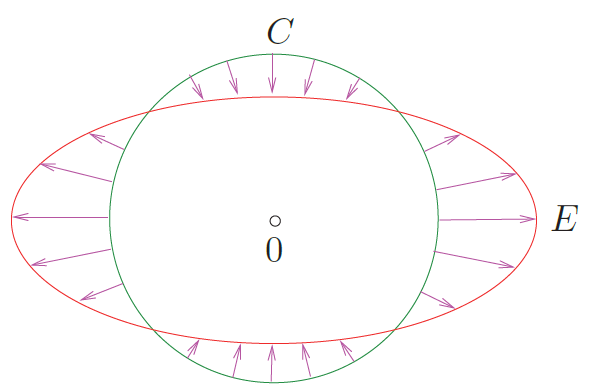
\includegraphics[width=0.4\textwidth]{./figs/fig-5-17}
\end{center}
\caption{$\mathbb C\setminus \{0\}$-호모토픽한 경로 $E$와 $C$}
\label{fig-5-17}
\end{figure}

따라서 코시 적분정리에 의해 $\dint_E \dfrac 1z dz = \dint_C \dfrac1z dz = 2\pi i$이고,
\begin{align*}
2\pi i &= \int_E \dfrac 1z dz = \int_0^{2\pi} \dfrac1{a\cos\theta +i b\sin\theta}
\cdot(-a\sin\theta + ib\cos\theta)d\theta \\
&= \int_0^{2\pi} \dfrac{(-a\sin\theta +ib\cos\theta)(a\cos\theta -ib\sin\theta)}
{a^2(\cos\theta)^2 + b^2(\sin\theta)^2}d\theta \\
&= \int_0^{2\pi} \dfrac{(b^2-a^2)(\cos\theta)(\sin\theta)+iab((\cos\theta)^2+(\sin\theta)^2)}
{a^2(\cos\theta)^2 + b^2(\sin\theta)^2}d\theta \\
&= \int_0^{2\pi} \dfrac{(b^2-a^2)(\cos\theta)(\sin\theta)+iab\cdot 1}
{a^2(\cos\theta)^2 + b^2(\sin\theta)^2}d\theta.
\end{align*}
허수부를 비교하면,
$\dint_0^{2\pi} \dfrac1{a^2(\cos\theta)^2 + b^2(\sin\theta)^2}d\theta = \dfrac{2\pi}{ab}$.

\subsection*{연습문제 \ref{ex-3-20}}

\begin{figure}[h!]
\begin{center}
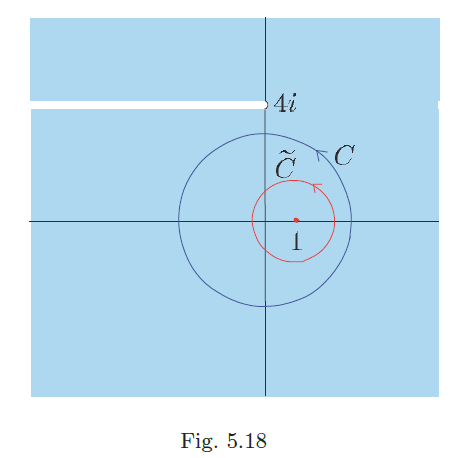
\includegraphics[width=0.4\textwidth]{./figs/fig-5-18}
\end{center}
\caption{적분경로 $C$, $\tilde C$}
\label{fig-5-18}
\end{figure}

그림 \ref{fig-5-18}을 참고하라.

\begin{itemize}
\item[(1)]  $z\mapsto \Log(z-4i)$는 $\mathbb C \setminus \{r+4i \,:\, r\le0\}$에서
복소해석함수이다. 따라서 코시 적분정리를 쓰면,
\[
\int_C \Log (z-4i)dz = 0.
\]
\item[(2)] $\tilde C$가 중심이 $1$이고 반지름 $r>0$인 원이라 하면,
\[
\int_{\tilde C} \dfrac1{z-1} dz = 2\pi i
\]
임을 알고 있다.
$1/(\cdot -1)$이 $\mathbb C\setminus\{1\}$에서 복소해석함수이고
원형경로 $C$와 $\tilde C$는 $\mathbb C\setminus\{1\}$-호모토픽이므로,
코시 적분정리에 의해,
\[
\int_C \dfrac1{z-1} dz = \int_{\tilde C} \dfrac1{z-1}dz = 2\pi i.
\]
\item[(3)] 
\begin{align*}
i^{z-3} &= \exp((z-3)\Log i) = \exp\left( (z-3)\left( \log 1 + i\dfrac\pi2\right)\right) \\
&= \exp\left( (z-3)\left(0+i\dfrac\pi2\right)\right) \\
&= \exp\left( i\dfrac\pi2 \cdot(z-3)\right).
\end{align*}
따라서 $z\mapsto i^{z-3}$은 전해석함수이다.
코시 적분정리에 의해
\[
\int_C i^{z-3}dz = 0.
\]
\end{itemize}

\subsection*{연습문제 \ref{ex-3-21}}

\begin{itemize}
\item[(1)] 
\[
\varphi'(t) = \exp\left( \int_0^t \dfrac{\gamma'(s)}{\gamma(s)}ds \right)
\cdot \dfrac d{dt}\left( \int_0^t \dfrac{\gamma'(s)}{\gamma(s)}ds \right) 
= \varphi(t)\cdot \dfrac{\gamma'(t)}{\gamma(t)}
\]
에서 $\varphi'\gamma - \varphi\gamma' = 0$이고,
\[
\dfrac d{dt} \left( \dfrac\varphi \gamma \right) 
= \dfrac{\varphi'\gamma - \varphi\gamma'}{\gamma^2} = \dfrac0{\gamma^2} = 0.
\]
따라서 $\dfrac{\varphi(0)}{\gamma(0)}=\dfrac{\varphi(1)}{\gamma(1)}$.
그런데, $\gamma$가 닫힌경로이므로 $\gamma(0)=\gamma(1)$이므로,
\[
\varphi(1) = \varphi(0) = \exp\left( \int_0^0 \dfrac{\gamma'(s)}{\gamma(s)}ds \right)
= \exp(0) = 1.
\]
결론적으로, $w(\gamma) \in\mathbb Z$.
\item[(2)] $\Gamma_1(t) = \exp(2\pi i t)$ ($t\in[0,1]$)의 회전수는
\begin{align*}
w(\Gamma_1) &= \dfrac1{2\pi i} \int_0^1 \dfrac{\Gamma_1'(t)}{\Gamma_1(t)} dt \\
&=\dfrac1{2\pi i} \int_0^1 \dfrac{2\pi i\exp(2\pi i t)}{\exp(2\pi i t)}dt \\
&=\dfrac1{2\pi i} \cdot 2\pi i  = 1.
\end{align*}
\item[(3)]  $(\gamma_1\cdot\gamma_2)'(t) = \gamma_1'(t)\gamma_2(t) +
\gamma_1(t)\gamma_2'(t)$, $t\in[0,1]$이므로,
\begin{align*}
w(\gamma_1\cdot\gamma_2)
&= \dfrac1{2\pi i} 
\int_0^1 \dfrac{(\gamma_1\cdot\gamma_2)'(t)}{(\gamma_1\cdot\gamma_2)(t)}dt\\
&= \dfrac1{2\pi i} \int_0^1 \dfrac{\gamma_1'(t)\gamma_2(t) +\gamma_1(t)\gamma_2'(t)}
{(\gamma_1\cdot\gamma_2)(t)}dt \\
&= \dfrac1{2\pi i} \int_0^1 \dfrac{\gamma_1'(t) \cancel{\gamma_2(t)}}
{\gamma_1(t) \cancel{\gamma_2(t)}}dt 
+ \dfrac1{2\pi i} \int_0^1 \dfrac{\cancel{\gamma_1(t)}\gamma_2'(t)}
{\cancel{\gamma_1(t)}\gamma_2(t)}dt  \\
&= w(\gamma_1) + w(\gamma_2).
\end{align*}
\item[(4)] $\Gamma_m = \Gamma_1 \cdot\cdots\cdot \Gamma_1$ ($m$번 곱)이므로
\begin{align*}
w(\Gamma_m) &= w(\Gamma_1) + \cdots + w(\Gamma_1) \ \ (m\text{번}) \\
&= m\cdot w(\Gamma_1) = m\cdot 1 = m.
\end{align*}
\item[(5)] 함수 $\varphi:[0,1]\to \mathbb R$를 
원점에서 $\gamma_0(t)$까지의 거리 $\varphi(t) = |\gamma_0(t)|$, $t\in[0,1]$로 정의하자.
$\gamma_0$가 $0$을 지나지 않고, $\varphi$는 연속함수이기 때문에
최솟값 $d_0$ ($d_0>0$)를 갖는다.
$\delta = d_0/2 >0$로 택하자.
$\gamma$가 
\[
\|\gamma - \gamma_0\| := \max_{t\in[0,1]} | \gamma(t) - \gamma_0(t)| < \delta
\]
를 만족하는 매끄러운 닫힌경로라고 하자.
그러면
$\gamma$가 $\gamma_0$와 $\mathbb C\setminus \{0\}$-호모토픽함을 증명하고자 한다.
$H:[0,1]\times[0,1]\to \mathbb C\setminus\{0\}$를 
$H(t,s) = (1-s)\gamma_0(t) + s\gamma(t)$, $t,s\in[0,1]$로 정의하면
$H$는 연속함수이고,
\begin{align*}
H(t,0) &= \gamma_0(t), \quad t\in[0,1],\\
H(t,1) &= \gamma(t), \quad t\in[0,1],\\
H(0,s) &= (1-s)\gamma_0(0) + s\gamma(0) \\
&= (1-s)\gamma_0(1) + s\gamma(1)  = H(1,s), \quad s\in[0,1].
\end{align*}

또한, $H(t,s)$는 $0$이 될 수 없다. 왜냐하면,
$\gamma_0(t)$와 $\gamma(t)$의 볼록결합이기 때문이다.
어떤 $t,s$에 대하여 $(1-s)\gamma_0(t)+s\gamma(t)=0$라면
모순에 도달하게 된다. 그림 \ref{fig-5-19}\를 참고하라.

\begin{figure}[h!]
\begin{center}
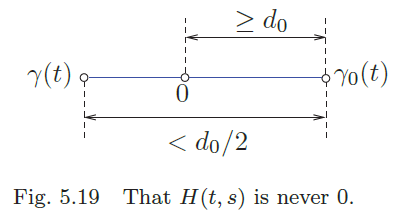
\includegraphics[width=0.4\textwidth]{./figs/fig-5-19}
\end{center}
\caption{$H(t,s)$는 $0$이 될 수 없다.}
\label{fig-5-19}
\end{figure}
직접 계산해보면,
\begin{align*}
1\cdot \dfrac{d_0}2 &> s|\gamma_0(t) - \gamma(t)|
= | \gamma_0(t) - 
\underbrace{((1-s)\gamma_0(t) + s\gamma(t))}_{=0\text{인 $t,s$를 선택할 수 있다면}}
| = |\gamma_0(t) - 0| \\
&= |\gamma_0(t)| \ge d_0.
\end{align*}
그러면, 코시 적분정리에 의해
\[
w(\gamma) = \dfrac1{2\pi i} \int_\gamma \dfrac1z dz 
= \int_{\gamma_0} \dfrac1z dz  = w(\gamma_0).
\]
\end{itemize}

\subsection*{연습문제 \ref{ex-3-22}}

\begin{figure*}[h!]
\begin{center}
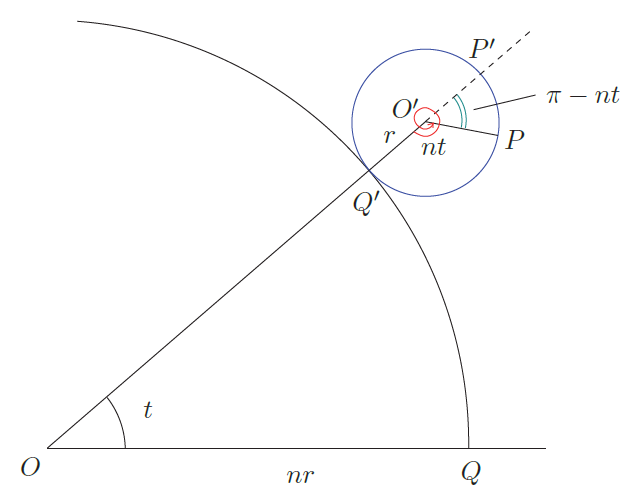
\includegraphics[width=0.4\textwidth]{./figs/fig-s-0-10}
\end{center}
%\caption{적분경로 $C$, $\tilde C$}
%\label{fig-5-18}
\end{figure*}

\begin{itemize}
\item[(1)] 큰 원의 각 $\angle Q'OQ$에 대응하는 호의 길이는 $t\cdot nr$이다.
작은 동전이 미끄러지지 않고 돌아갈 때, $O'P$와 $OO'$이 이루는 각은
$(t\cdot nr)/r = n\cdot t$이다. 그림에서 $O' \equiv (nr+r)\exp(it)$이고
\begin{align*}
P & \equiv (nr+r)\exp(it) + 
\underbrace{\exp(-i(\pi-nt))}_{\text{시계방향으로 회전}}\cdot
\underbrace{r\exp(it)}_{O'P'} \\
&=(n+1)r\exp(it) + (-1)\cdot r\cdot \exp((n+1)it).
\end{align*}
\item[(2)] 에피사이클로이드 곡선 $\gamma$로 둘러싸인 영역의 면적은
 \begin{align*}
\dfrac1{2i} \int_\gamma \bar z dz 
&= \dfrac1{2i}\int_0^{2\pi} \overline{r\left( (n+1)\exp(it)-\exp((n+1)it)\right)}\cdot \\
&\qquad\qquad r\left((n+1)i\exp(it) - (n+1)i\exp((n+1)it)\right)dt \\
&= \dfrac1{2i} \int_0^{2\pi} r^2\left( (n+1)\exp(-it) - \exp(-(n+1)it)\right)\cdot  \\
&\qquad\qquad (n+1)i\left(\exp(it) - \exp((n+1)it)\right)dt \\
&= \dfrac{(n+1)r^2}2 \int_0^{2\pi} ((n+1) -(n+1)\exp(int) - \exp(-int) +1)dt \\
&= \dfrac{(n+1)r^2}2 ((n+1) \cdot 2\pi + 0+0 + 2\pi) \\
&= (n+1)r^2\pi(n+2) = \pi r^2 (n+1)(n+2).
\end{align*}
\end{itemize}

\subsection*{연습문제 \ref{ex-3-23}}

$z\in D:= \mathbb C\setminus\{0\}$에 대하여 $f(z) = 1/z$로 정의하자.
그러면, $f$는 $D$에서 부정적분(원시함수)을 가질 수 없다.
(예제 \ref{example-3-7}\과 연습문제 \ref{ex-3-16 }\을 참고하라.)

\subsection*{연습문제 \ref{ex-3-24}}

$\gamma(t) = \exp(it)$, $t\in[0,1]$이라 하면,
\begin{align*}
\int_\gamma \dfrac i{(z-a)(az-1)}dz 
&= \int_0^{2\pi} \dfrac{i}{(\exp(it) -a)(a\exp(it)-1)}i\exp(it)dt \\
&= \int_0^{2\pi} \dfrac{-\exp(it)}{(\exp(it) -a)(a-\exp(-it))\exp(it)}dt \\
&= \int_0^{2\pi} \dfrac{1}{(\exp(it) -a)(\exp(-it)-a)}dt \\
&= \int_0^{2\pi} \dfrac1{|\exp(it)-a|^2}dt \\
&= \int_0^{2\pi} \dfrac1{((\cos t)-a)^2 + (\sin t)^2}dt \\
&= \int_0^{2\pi} \dfrac1{1-2a\cos t + a^2}dt.
\end{align*}
$0<a<1$일 때,
함수 $z\mapsto i/(ax-1)$이 단위원 $\gamma$를 포함하는 원판에서 복소해석함수이므로,
코시 적분공식에 의해
\[
\dfrac1{2\pi i} \int_\gamma \dfrac{\frac{i}{az-1}}{z-a}dz = \dfrac{i}{az-1}\Big|_{z=a}
= \dfrac i{a^2-1}.
\]
따라서,
$\dint_0^{2\pi} \dfrac 1{1-2a\cos t +a^2}dt
= \dint_\gamma \dfrac{\frac{i}{az-1}}{z-a}dz 
= 2\pi i \cdot \dfrac i{a^2-1} = \dfrac{2\pi}{1-a^2}$.

\subsection*{연습문제 \ref{ex-3-25}}

\begin{figure*}[h!]
\begin{center}
\includegraphics[width=0.7\textwidth]{./figs/fig-s-0-11}
\end{center}
%\caption{적분경로 $C$, $\tilde C$}
%\label{fig-5-18}
\end{figure*}

\begin{itemize}
\item[(1)] $\dint_\gamma \dfrac{\exp z}{z-1}dz = 2\pi i \exp z \Big|_{z=1}
= 2\pi i \exp 1 = 2\pi i  e$.
\item[(2)] $\dint_\gamma \dfrac{z^2+1}{z^2-1}dz 
= \dint_\gamma \dfrac {\frac{z^2+1}{z+1}}{z-1}dz
= 2\pi i \dfrac{z^2+1}{z+1} \Big|_{z=1} = 2\pi i \dfrac{1^2+1}{1+1} = 2\pi i$.
\item[(3)] $\dint_\gamma \dfrac{z^2+1}{z^2-1}dz = 0$.
\item[(4)] $\dint_\gamma \dfrac{z^2+1}{z^2-1}dz 
= \dint_\gamma \dfrac{\frac{z^2+1}{z-1}}{z-(-1)}dz 
= 2\pi i \dfrac{z^2+1}{z-1} \Big|_{z=-1} = 2\pi i \dfrac{(-1)^2+1}{-1-1} = -2\pi i$.
\item[(5)] $\dint_\gamma \dfrac{z^2+1}{z^2-1}dz 
= \dint_\gamma \dfrac{z^2+1}2 \left(\dfrac1{z-1} - \dfrac1{z+1}\right)dz$
\begin{align*}
\quad &= \int_\gamma \dfrac{\frac{z^2+1}2}{z-1}dz 
- \int_\gamma \dfrac{\frac{z^2+1}2}{z-(-1)}dz 
= 2\pi i \dfrac{z^2+1}2\Big|_{z=1} - 2\pi i \dfrac{z^2+1}2 \Big|_{z=-1} \\
&= 2\pi i(1) - 2\pi i (1) = 0.
\end{align*}
\end{itemize}

\subsection*{연습문제 \ref{ex-3-26}}

$F$가 부정적분이라고 하자.
원 $|z-0| = \frac12$을 반시계방향으로 도는 닫힌경로 $\gamma$를 생각하자.
경로적분의 기본정리에 의해,
\[
\dint_\gamma \dfrac1{z(z^2-1)}dz = \int_\gamma F'(z)dz = 0.
\]
한편,  코시 적분공식을 쓰면,
\[
\int_\gamma \dfrac1{z(z^2-1)}dz = \int_\gamma  \dfrac{\frac1{z^2-1}}{z-0}dz
= 2\pi i \dfrac1{z^2-1}\Big|_{z=0} = 2\pi i \dfrac1{0^2-1} = - 2\pi i.
\]
따라서 모순에 도달하게 되어
\[
\dfrac1{z(z^2-1)}
\]
은 $\{z\in\mathbb C\,:\, 0<|z|<1\}$에서 부정적분을 가질 수 없다.

\subsection*{연습문제 \ref{ex-3-27}}

\begin{figure}[h!]
\begin{center}
\includegraphics[width=0.4\textwidth]{./figs/fig-5-20}
\end{center}
\caption{경로 $\sigma=S+T$}
\label{fig-5-20}
\end{figure}

\begin{itemize}
\item[(1)] 코시 적분공식에 의해
\begin{align*}
\int_\sigma F(z) dz &= \int_\sigma \dfrac{\exp(iz)}{z^2+1}dz
= \int_\sigma \dfrac{\frac{\exp(iz)}{z+1}}{z-1}dz
= 2\pi i \dfrac{\exp(iz)}{z+1}\Big|_{z=i} \\
&= 2\pi i \dfrac{\exp(i\cdot i)}{i+i} = 2\pi i \dfrac{e^{-1}}{2i} = \dfrac\pi e.
\end{align*}

\item[(2)] $z=x+iy$, $x,y$는 실수이고, $y\ge0$라 하자. 그러면,
\[
|\exp(iz)| = |\exp(i(x+iy))| = |\exp(-y+ix)| = e^{-y} \le 1.
\]
따라서,
\[
|F(z)| = \dfrac{|\exp(iz)|}{|z^2+1|} \le \dfrac1{|z^2+1|}.
\]
한편, $|z^2| - |-1| \le |z^2-(-1)| = |z^2+1|$이므로,
$|z|\ge\sqrt{2}$이면,
\[
|F(z)| \le \dfrac1{|z^2+1|} \le \dfrac1{|z|^2-1} \le \dfrac2{|z|^2}.
\]
부등식을 만들 때 $|z^2|\ge 2$이면, $|z|^2\le 2|z|^2 -2$임을 이용하였다.
($|z|\ge\sqrt{2}$이면 이 조건이 만족된다)
\item[(3)] 
\begin{align*}
\left| \int_T F(z)dz \right| 
\le 2\pi R\cdot \max_{z\in T} |F(z)| &\le 2\pi R\cdot \dfrac 2{R^2} 
\quad (R\ge\sqrt{2}\text{일 때})\\
&= \dfrac{4\pi}R \stackrel{R\to\infty}{\longrightarrow} 0.
\end{align*}
따라서 $\Lim_{R\to\infty} \int_T F(z) dz = 0$.
\[
\int_S F(z)dz = \int_\sigma F(z) dz - \int_T F(z)dz = \dfrac \pi 2 -  \int_T F(z)dz
\]
이므로,  $\Lim_{R\to\infty} \int_S F(z)dz = \dfrac\pi e -\Lim_{R\to\infty} \int_T F(z)dz
= \dfrac \pi e - 0 = \dfrac \pi e$.
\item[(4)] $S(x)=x$, $x\in[-R,R]$이라 하자. 그러면,
\begin{align*}
\int_S F(z)dz &= \int_{-R}^R \dfrac{\exp(ix)}{x^2+1}\cdot 1 dx
=\int_{-R}^R \dfrac{\cos x}{x^2+1} dx 
+ i\int_{-R}^R \dfrac{\sin x}{x^2+1} dx \\
&= \int_{-R}^R \dfrac{\cos x}{x^2+1}dx  + 0
\end{align*}
마지막 등식은 $\dfrac{\sin x}{x^2+1}$이 기함수라는 성질을 이용하였다.
결론적으로,
\[
\Lim_{R\to\infty} \int_{-R}^R \dfrac{\cos x}{x^2+1}dx
= \Lim_{R\to\infty}\int_S F(z)dz = \dfrac \pi e.
\]
\end{itemize}

\subsection*{연습문제 \ref{ex-3-28}}

전해석함수 $\exp z$와 중심이 $0$이고 빈지름 $1$인 원형경로
$C:[0,2\pi] \to \mathbb C$가 $C(\theta) = \exp(i\theta)$, $\theta \in [0,2\pi]$로 
주어졌다고 하자.
코시  적분공식에 의하여,
\[
\dfrac1{2\pi i} \int_C \dfrac{\exp z}{z-0}dz = \exp z\Big|_{z=0} = \exp 0 = 1.
\]

%





%===[salt] 4장
% !TEX root = ./CA_solution.tex

\section*{4장 - 연습문제 풀이}

\subsection*{연습문제 \ref{ex-4-1}}

$\Sum_{n=1}^\infty a_n$이 수렴하면,
$\Sum_{n=1}^\infty \Re(a_n)$과 $\Sum_{n=1}^\infty \Im(a_n)$도 각각 수렴한다.
따라서 $\Lim_{n\to\infty} \Re(a_n) = 0$이고, $\Lim_{n\to\infty} \Im(a_n) = 0$이다.
이로부터 $\Lim_{n\to\infty} a_n = 0$이다.

\subsection*{연습문제 \ref{ex-4-2}}

$\Sum_{n=1}^\infty |a_n|$이 수렴한다고 하자.
모든 $ n\in \mathbb N$에 대하여
$\Re(a_n) \le |a_n|$, $\Im(a_n) \le |a_n|$이므로
비교판정법에 의해
\[
\Sum_{n=1}^\infty \Re(a_n), \quad \Sum_{n=1}^\infty \Im(a_n)
\]
이 수렴한다.
따라서 $\Sum_{n=1}^\infty a_n$도 수렴한다.

\subsection*{연습문제 \ref{ex-4-3}}

$s_n:= 1+z+\cdots + z^{n-1}+z^n$이라 하면,
$z s_n = z + z^2 + \cdots + z^n + z^{n+1}$이므로
$(1-z)s_n = 1- z^{n+1}$이다.
$|z|<1$에서  $z\ne1$이므로
\begin{equation}\label{eq-5-21}
s_n = 1+z+\cdots + z^{n-1}+z^n = \dfrac{1-z^{n+1}}{1-z}.
\end{equation}
따라서
\[
\Lim_{n\to\infty} s_n = \lim_{n\to\infty}\dfrac{1-z^{n+1}}{1-z}
= \dfrac{1-0}{1-z} = \dfrac1{1-z}
\]
이므로 $\Sum_{n=0}^\infty z^n$이 수렴하고
$\Sum_{n=0}^\infty z^n = \Lim_{n\to\infty} s_n = \dfrac1{1-z}$이다.
(이 증명을 위해 $|z|<1$에서
\[
\lim_{n\to\infty} z^{n+1} = 0
\]
을 이용하였다.  이 결과는
$r:=|z|<1$이므로, $|z^{n+1} -0| = |z|^{n+1} \stackrel{n\to\infty}{\longrightarrow }0$로부터
얻어진다.)

\subsection*{연습문제 \ref{ex-4-4}}

자연수 $n\in\mathbb N$에 대하여 
$s_n:= 1+2z + 3z^2 + \cdots + (n-1)z^{n-2} + nz^{n-1}$이라 하자.
그러면 $zs_n = z + 2z^2 + \cdots + (n-1)z^{n-1} + nz^n$이다.
따라서
\[
(1-z)s_n= 1 + z + z^2 + \cdots + z^{n-1} - nz^n
= \dfrac{1-z^n}{1-z}  - nz^n.
\]
따라서
\[
s_n = \dfrac{1-z^n}{(1-z^2}  - \dfrac{nz^n}{1-z}.
\]
(이 결과는 식 \eqref{eq-5-21}의 양변을 $z$에 대하여 미분해서 얻을 수도 있다.)

$r:=|z|$ ($0\le r < 1$)이라 하면,
\[
r = \dfrac1{1+h}
\]
여기서 $h:=\dfrac1r-1>0$이다.
\[
(1+h)^n = 1 + {n\choose 1}h + {n \choose 2}h^2 + \cdots
+ {n \choose n}h^n \ge {n \choose 2}h^2 = \dfrac{n\cdot(n-1)}2 \cdot h^2
\]
에서
\[
0\le nr^n \dfrac n{(1+h)^n} \le n \cdot \dfrac2{n\cdot(n-1)\cdot h^2}
= \dfrac 2{(n-1)\cdot h^2}
\]
이므로
조임정리(Sandwitch theorem)에 의하여 $\Lim_{n\to\infty} nr^n = 0$이다.
결론적으로,
\[
\Lim_{n\to\infty}  s_n = \Lim_{n\to\infty} \left( \dfrac{1-z^n}{(1-z)^2}
- \dfrac{nz^n}{1-z} \right)
= \dfrac{1-0}{(1-z)^2} - \dfrac0{1-z} = \dfrac1{(1-z)^2}.
\]

\subsection*{연습문제 \ref{ex-4-5}}

\begin{align*}
\left| \dfrac1{n^s} \right| &= \left| \dfrac1{\exp(s\cdot \Log(n))} \right|
= \left| \dfrac1{\exp(s\cdot\log n)}\right| \\
&= \dfrac1{e^{\Re(s\cdot \log n)}} = \dfrac1{e^{(\log n)\cdot(\Re(s))}}
= \dfrac1{(e^{\log n})^{\Re(s)}} = \dfrac1{n^{\Re(s)}}.
\end{align*}

$p>1$이면 $\Sum_{n=1}^\infty \dfrac1{n^p}$이 수렴함을 이용하면,
$\Re(s)>1$에 대하여
\[
\sum_{n=1}^\infty \dfrac1{n^{\Re(s)}}
\]
가 수렴한다. 따라서  $\Re(s)>1$인 영역에서
\[
\sum_{n=1}^\infty \dfrac1{n^{s}}
\]
은 절대수렴하므로, 당연히 수렴한다.

\subsection*{연습문제 \ref{ex-4-6}}

$L\ne0$이라고 하자.
$|z|< 1/L$인 모든 $z$에 대하여, 
$N$이 충분히 클 때 $n>N$이면
$\sqrt[n]{|c_nz^n|}  = \sqrt[n]{|c_n|}|z| \le q <1$를 만족하는 $q<1$가 존재한다.
이는 $\sqrt[n]{|c_n|}|z| \stackrel{n\to\infty}{\longrightarrow}L|z|<1$로부터 얻어진다.
(예를 들어 $q=(L|z|+1)/2 <1$로 잡으면 된다.)

$L=0$이면, 
임의의(고정된) $z\in \mathbb C$에 대하여
$n>N$이면 $\sqrt[n]{|c_nz^n|} = \sqrt[n]{|c_n|}|z| \le q < 1$을 항상 만족하는 $q<1$가 존재한다.
이는 $\sqrt[n]{|c_n|}|z| \stackrel{n\to\infty}{\longrightarrow}0|z|=0<1$로부터 얻어진다.
(예를 들어 $q=1/2<1$로 잡으면 된다.)
근판정법을 쓰면 제곱급수가 수렴함을 알 수 있다.

한편, $L\ne0$이고 $|z|>1/L$인 경우를 생각하면
$N$이 충분히 클 때 모든 $n>N$에 대하여
$\sqrt[n]{|c_nz^n|}  = \sqrt[n]{|c_n|}|z| >1$가 성립한다.
이는 $\sqrt[n]{|c_n|}|z| \stackrel{n\to\infty}{\longrightarrow}L|z|>1$로부터 얻어진다.
다시 근판정법을 쓰면 이 경우 제곱급수가 발산함을 알 수 있다.

\subsection*{연습문제 \ref{ex-4-7}}

$z=0$일 때 급수가 $0$으로 수렴함은 자명하다.
$z\ne 0$라고 가정하자. 그러면, $N>1/|z|$인 
$N\in\mathbb N$를 선택할 수 있다.
$n>N$에 대하여 $|nz|>N|z|>1$이고
$|n^nz^n -0| = |nz|^n >1^n = 1$이므로
\[
\neg \left( \lim_{n\to\infty} n^n z^n = 0 \right).
\]
따라서 $z\ne0$이면, $\Sum_{n=1}^\infty n^n z^n$은 발산한다.

\subsection*{연습문제 \ref{ex-4-8}}

$\Lim_{n\to\infty} \sqrt[n]{\dfrac1{n^n}} = \Lim_{n\to\infty} \dfrac1n = 0$이므로
\[
\sum_{n\to\infty} \dfrac{z^n}{n^n}
\]
의 수렴반경은 무한대이고 이 제곱급수는 모든 $z\in\mathbb C$에 대하여 수렴한다.

\subsection*{연습문제 \ref{ex-4-9}}

\begin{itemize}
\item[(1)] 
\[
\lim_{n\to\infty} \left| \dfrac{\dfrac{(-1)^{n+1}}{n+1}}{\dfrac{(-1)^n}n} \right|
= \lim_{n\to\infty} \dfrac n{n+1} = 1
\]
이므로 $\Sum_{n=1}^\infty \dfrac{(-1)^n}n z^n$의 수렴반경은 $1$이다.

\item[(2)] 
\[
\lim_{n\to\infty} \left| \dfrac{(n+1)^{2012}}{n^{2012}} \right|
= \lim_{n\to\infty} \left( 1+ \dfrac1{n} \right)^{2012} = 1
\]
이므로 $\Sum_{n=1}^\infty n^ {2012} z^n$의 수렴반경은 $1$이다.

\item[(3)] 
\[
\lim_{n\to\infty} \left| \dfrac{\dfrac{1}{(n+1)!}}{\dfrac1{n!}} \right|
= \lim_{n\to\infty} \dfrac1{n+1} = 0
\]
이므로 $\Sum_{n=1}^\infty \dfrac1{n!}z^n$의 수렴반경은 무한대이다.
\end{itemize}

\subsection*{연습문제 \ref{ex-4-10}}

$|z|<1$에 대하여
\[
f(z):= 1+2z+ 3z^3 + 4z^3 + \cdots = \dfrac 1{(1-z)^2}
\]
이므로 
\[
zf(z) = g(z) := z + 2z^2 + 3z^3 + 4z^4 + \cdots = \dfrac z{(1-z)^2}
\]
임을 알고 있다.
따라서 $g(z):= z+2z^2+3z^3 + 4z^4 + \cdots$이 $|z|<1$에서 수렴하므로
$g$는 원판 $|z|<1$에서 복소해석함수이고
$g'(z) = 1 + 2^2z + 3^2z^2 + 4^2z^3 + \cdots$이다.
한편,
\[
g(z) = zf(z) = \dfrac z{(1-z)^2}
\]
이므로
\[
g'(z) = \dfrac d{dz} \left( \dfrac z{(1-z)^2} \right)
= 1\cdot \dfrac1{(1-z)^2} + z\cdot\dfrac 2{(1-z)^3}
= \dfrac{1-z+2z}{(1-z)^3} = \dfrac{1+z}{(1-z)^3}
\]
이 원하는 결과이다.

\subsection*{연습문제 \ref{ex-4-11}}

\begin{itemize}
\item[(1)] 거짓.
예를 들면, $\left\{ z\in\mathbb C\,:\, \Sum_{n=1}^\infty \dfrac{z^n}{n^2} \text{수렴한다} \right\}
= \left\{ z\in\mathbb C\,:\, |z|\le 1\right\}$은 ``닫힌''영역이다.
\item[(2)] 참.
\item[(3)] 거짓. 
예를 들면, $\Sum_{n=1}^\infty \dfrac{(-1)^n}n z^n$은 $z=1$에서 수렴하지만
$z=-1$에서는 발산한다.
\item[(4)] 거짓. (3)의 예를 참고하라.
\item[(5)] 참. (3)의 예를 참고하라.
\item[(6)] 참. 예를 들면, $\Sum_{n=1}^\infty \dfrac{z^n}{n^2}$.
\item[(7)] 참. 수렴반경은 $1$보다 작거나 같고, $|1+i| = \sqrt{2} >1$이다.
\end{itemize}

\subsection*{연습문제 \ref{ex-4-12}}

$\sin 0 = 0$, $\cos 0 =1$이고,
\[
\dfrac{d^{2n}}{dz^{2n}} \sin z = (-1)^n \sin z,
\quad
\dfrac{d^{2n+1}}{dz^{2n+1}} \sin z = (-1)^n \cos z
\]
이므로 
\[
\sin z = \sum_{n=0}^\infty \dfrac1{n!} \left(\dfrac{d^n}{dz^n} \sin z \right)\Big|_{z=0}
= z - \dfrac{z^3}{3!} + \dfrac{z^5}{5!} - \cdots
\]
같은 방법으로 $\cos z = 1 - \dfrac{z^2}{2!} + \dfrac{z^4}{4!} - \cdots$.
다른 방법으로 구해보면,
\[
\cos z = \dfrac{\exp(iz)  + \exp(-iz)}2 
= \dfrac12 \left( \sum_{n=0}^\infty \dfrac1{n!}i^nz^n 
+ \sum_{n=0}^\infty \dfrac1{n!}(-1)^ni^nz^n \right)
\]
이므로, $i^{2n} = (-1)^n$을 이용하면,
\begin{align*}
\cos z &= \dfrac12 \left(
1+ iz - \dfrac{z^2}{2!} - \dfrac{iz^3}{3!} + \dfrac{z^4}{4!} \right.
+ \dfrac{iz^5}{5!} - \dfrac{z^6}{6!}  + \cdots \\
&\qquad\left. +1 - iz - \dfrac{z^2}{2!} + \dfrac{iz^3}{3!} + \dfrac{z^4}{4!} 
- \dfrac{iz^5}{5!} - \dfrac{z^6}{6!}  + \cdots \right) \\
&= 1 - \dfrac1{2!}z^2 + \dfrac1{4!}z^4 - \dfrac1{6!}z^6 + \cdots.
\end{align*}

\subsection*{연습문제 \ref{ex-4-13}}

$p(z) = z^6 -z^4 +z^2 -1$, $z\in \mathbb C$라 하면,
\begin{align*}
& p'(z) = 6z^5 - 4z^3 +2z, \\
& p''(z) = 30z^4 -12z^2 + 2, \\
&p'''(z) = 120z^3 - 24z, \\
&p^{(4)}(z) = 360z^2 - 24, \\
&p^{(5)}(z) = 720z, \\
&p^{(6)}(z) = 720, \\
&p^{(7)}(z) = p^{(8)} = \cdots = 0
\end{align*}
이므로,
\begin{align*}
&p(1) = 1-1+1-1 = 0, \\
&\dfrac{p'(1)}{1!} = 6 - 4 + 2 = 4, \\
&\dfrac{p''(1)}{2!} = \dfrac{30-12+2}{2} = 10, \\
&\dfrac{p'''(1)}{3!} = \dfrac{120-24}{6} = 16, \\
&\dfrac{p^{(4)}(1)}{4!} = \dfrac{360-24}{24} = 14, \\
&\dfrac{p^{(5)}(1)}{5!} = \dfrac{720}{120} = 6, \\
&\dfrac{p^{(6)}(1)}{6!} = \dfrac{720}{720} = 1.
\end{align*}
따라서 모든 $z\in\mathbb C$에 대하여,
\begin{align*}
z^6&-z^4+z^2-1 \\
&= p(1) + \dfrac{p'(1)}{1!}(z-1) + \cdots + \dfrac{p^{(6)}(1)}{6!}(z-1)^6 + 0 \\
&= 4(z-1) + 10(z-1)^2 + 16(z-1)^3 + 14(z-1)^4 + 6(z-1)^5 + (z-1)^6.
\end{align*}

\subsection*{연습문제 \ref{ex-4-14}}

\begin{itemize}
\item[(1)] 
단순연결영역 $\mathbb C$에서
$z\mapsto \exp(z^2)$은 부정적분을 가지며, 이를 $g$라 하면
\[
f(z) = \int_{\gamma_{0z}} \exp(\zeta^2) d\zeta 
= \int_{\gamma_{0z}} g'(\zeta) d\zeta = g(z) - g(0).
\]
따라서 $f'(z) = g'(z) = \exp(z^2) = \Sum_{n=0}^\infty \dfrac1{n!}z^{2n}$.
\[
\dfrac1{(2n)!} \dfrac{d^{2n}}{dz^{2n}}f'(z) \Big|_{z=0} = \dfrac1{n!}, 
\quad
\dfrac1{(2n+1)!} \dfrac{d^{2n+1}}{dz^{2n+1}}f'(z) \Big|_{z=0} = 0
\]
이므로
$f^{(2n+1)}(0) = \dfrac{(2n)!}{n!}$, $f^{(2n+2)}(0) = 0$이고, $f(0)=0$이다.
따라서,
\[
f(z) = \sum_{n=0}^\infty \dfrac{f^{(n)}(0)}{n!} z^n 
= \sum_{n=0}^\infty \dfrac{f^{(2n+1)}(0)}{(2n+1)!} z^{2n+1}
= \sum_{n=0}^\infty \dfrac1{(2n+1)(n!)} z^{2n+1}.
\]
\item[(2)] 
$|z|<1$에 대하여,
\[
\dfrac1{z+1} = 1 - z + z^2 - z^4 + z^4 - \cdots
\]
이고 제곱급수는 수렴하는 영역에서 복소해석함수이고 항별미분이 가능하기 때문에
$|z|<1$에서
\[
- \dfrac1{(z+1)^2} = \dfrac d{dz}\dfrac1{z+1} = - 1 + 2z - 3z^2 + 4z^3 - \cdots
\]
양변에 $-z^2$을 곱하면, $|z|<1$에서
\[
 \dfrac{z^2}{(z+1)^2} =z^2 - 2z^3 + 3z^4 - \cdots
= \sum_{n=2}^\infty (-1)^n\cdot (n-1)\cdot z^n
\]
이므로 $c_0=c_1=0$이고, $c_n =(-1)^n\cdot(n-1)$ ($n\ge2$)이다.
\end{itemize}

\subsection*{연습문제 \ref{ex-4-15}}

$z\in\mathbb C$에 대하여 $R>|z|$을 잡으면,
\begin{align*}
|f^{(n+1)}(z)| &\le \dfrac{(n+1)!}{R^{n+1}}\cdot \max_{|z|\le R} |f(z)| \\
&\le \dfrac{(n+1)!}{R^{n+1}}\cdot \max_{|z|\le R} M\cdot |z|^n 
= \dfrac{(n+1)!}{R^{n+1}}\cdot M\cdot R^n = \dfrac{(n+1)!M}R.
\end{align*}
$R>|z|$의 선택을 임의로 크게 할 수 있기 때문에
$f^{(n+1)}(z) = 0$이다.
어떤 $z\in \mathbb C$을 선택해도 같은 결과를 얻기 때문에
$\mathbb C$ 전체에서 $f^{(n+1)} \equiv 0$이다.
테일러 정리에 의해,  모든 $z\in \mathbb C$에 대하여
\[
f(z) = \sum_{k=0}^\infty \dfrac{f^{(k)}(0)}{k!} (z-0)^k
= \sum_{k=0}^n \dfrac{f^{(k)}(0)}{k!} z^k.
\]
$f^{(n+1)}(0) = f^{(n+2)}(0) = f^{(n+3)}(0) = \cdots 0$이므로
$f$는 기껏해야 $n$차 다항식이다.

조건에서 $n=0$이면, $f$는 유계인 전해석함수이며
위의 결론에서 $f$는 상수함수이다 ($0$차 다항식).
따라서 특별히 $n=0$인 경우는 리우비유 정리와 일치한다.

\subsection*{연습문제 \ref{ex-4-16}}

코시 적분공식에 의해
\begin{align*}
\dfrac{2013!}{2\pi i}  \int_C \dfrac{\sin z}{z^{2013}}dz
&= \dfrac{d^{2012}}{dz^{2012}} \sin z \Big|_{z=0} \\
&= (-1)^{2012/2} \sin z\Big|_{z=0} \\
&=0
\end{align*}
이므로  $\dfrac{2013!}{2\pi i}  \dint_C \dfrac{\sin z}{z^{2013}}dz=0$.

\subsection*{연습문제 \ref{ex-4-17}}

$z_0$에서 $g$의 연속성에 의해
$|z-z_0|<\delta$에서 $g(z)\ne0$가 되도록 $R>0$보다 작은 $\delta>0$를 잡을 수 있다.
$f(z_0)=0$이고 $f(z) = (z-z_0)g(z)$ ($|z-z_0|<R$)이므로
$0<|z-z_0|<\delta$에서  $f(z)\ne0$이다.
근의 분류 정리에 의하여
$f$는 $z_0$에서 $\tilde m\in \mathbb N$ 중근을 갖고
$\tilde g(z_0)\ne0$인 복소해석함수 $\tilde g$가 존재한다.
이제 $|z-z_0|<R$에서
$(z-z_0)^{\tilde m} \tilde g(z) = (z-z_0)^m g(z)$가 성립한다.
$\tilde m = m$임을 증명해보자.
$\tilde m >m$이라면,
\[
0\ne g(z_0) = \lim_{z\to z_0} g(z) = \lim_{z\to z_0} (z-z_0)^{\tilde m - m}\tilde g(z_0) 
= 0\cdot \tilde g(z_0)= 0
\]
가 되어 모순에 도달한다. 반대로 $m>\tilde m$이면,
\[
0\ne \tilde g(z_0) = \lim_{z\to z_0} \tilde g(z) = \lim_{z\to z_0} (z-z_0)^{m - \tilde m} g(z_0) 
= 0\cdot g(z_0)= 0
\]
로 모순이다.
따라서, $m= \tilde m$이 되고, $z_0$는 $m$ 중근이다.

\subsection*{연습문제 \ref{ex-4-18}}

\begin{itemize}
\item[(1)] 
\[f(z) = (1+z^2)^4 = ((z-i)(z+i))^4
= (z-i)^4(z+i)^4
\]
이므로 $g(z):= (z+i)^4$이라 하면
$g$는 전해석함수이고 $g(i) = (2i)^4 = 16\ne 0$이고
$f(z) = (z-i)^4 g(z)$이다. 
따라서 $i$는 $f$의 $4$ 중근이다.
\item[(2)] 
\begin{align*}
f(2n\pi i) &= 1 - 1 = 0, \\
f'(2n\pi i) &= \exp z \Big|_{z=2n\pi i} = 1 \ne 0
\end{align*}
이므로  $f$의 근 $2n\pi i$의 차수는 $1$이다.
\item[(3)] $f(0)  = 1 - 1 + \dfrac12(0)^2 = 0$이고
\begin{align*}
f(z) &= \cos z - 1 + \dfrac12(\sin z)^2 = \cos z - 1 + \dfrac12 \cdot \dfrac{(1-\cos(2z))}2 \\
&= \cos z - \dfrac34 - \dfrac14\cos(2z) \\
&= \left( 1 - \dfrac{z^2}{2!} + \dfrac{z^4}{4!} - \dfrac{z^6}{6!} + \cdots \right)- \dfrac 34 \\
& \qquad -\dfrac14\left( 1 - \dfrac{4z^2}{2!} + \dfrac{16z^4}{4!} 
- \dfrac{2^6z^6}{6!} + \cdots \right) \\
&= \underbrace{\left(1-\dfrac34-\dfrac14\right)}_{0}
+ \underbrace{\left(-\dfrac1{2!} +\dfrac14\cdot\dfrac 4{2!}\right)}_{0} z^2
+ \underbrace{\left(\dfrac1{4!} - \dfrac14\cdot\dfrac {16}{4!}\right)}_{\ne 0} z^4 + \cdots
\end{align*}
이므로 근 $z_0$의 차수는 $4$이다.
\end{itemize}

\subsection*{연습문제 \ref{ex-4-19}}

원판에서 $z_0$와 다른 점 $z$를 잡으면 $f(z)\ne0$이다.
근의 분류 정리에서 $f(z)=(z-z_0)g(z)$로 쓸 수 있다.
여기서 $g$는 복소해석함수이고 $g(z_0)\ne0$이다.
\begin{align*}
\dfrac1{2\pi i}\int_\gamma \dfrac{zf'(z)}{f(z)}dz 
&= \dfrac1{2\pi i}\int_\gamma \dfrac{z(1\cdot g(z) + (z-z_0)\cdot g'(z))}{(z-z_0)g(z)}dz  \\
&= \dfrac1{2\pi i}\int_\gamma \dfrac{\dfrac{z(g(z) + (z-z_0)\cdot g'(z))}{g(z)}}{(z-z_0)}dz  \\
&= \dfrac{z(g(z) + (z-z_0)\cdot g'(z_0)}{g(z)}\Big|_{z=z_0} 
\quad\text{(코시 적분공식에 의해)} \\
&= \dfrac{z_0(g(z_0) + 0\cdot g'(z_0))}{g(z_0)} \\
&= z_0.
\end{align*}

\subsection*{연습문제 \ref{ex-4-20}}













\begin{figure}[h!]
\begin{center}
\includegraphics[width=0.4\textwidth]{./figs/fig-5-17}
\end{center}
\caption{$\mathbb C\setminus \{0\}$-호모토픽한 경로 $E$와 $C$}
\label{fig-5-17}
\end{figure}




 

%===[salt] 5장
% !TEX root = ./CA_solution.tex

\section*{5장 - 연습문제 풀이}

\subsection*{연습문제 \ref{ex-5-1}}

\begin{itemize}
\item[(1)] $(x,y)\in \mathbb R^2\setminus\{(0,0)\}$에 대하여
\begin{align*}
\dfrac{\partial u}{\partial x} &= \dfrac1{x^2+y^2} \cdot 2x = \dfrac{2x}{x^2+y^2} \\
\dfrac{\partial^2 u}{\partial x^2} &= \dfrac2{x^2+y^2} - \dfrac{2x}{(x^2+y^2)^2} \cdot (2x) 
= \dfrac{2y^2+2x^2-4x^2}{(x^2+y^2)^2} = \dfrac{2(y^2-x^2)}{(x^2+y^2)^2}.
\end{align*}
$x$, $y$에 대한 대칭식임을 이용하면
\[
\dfrac{\partial u}{\partial y}  = \dfrac{2y}{x^2+y^2}, \quad
\dfrac{\partial^2 u}{\partial y^2} = \dfrac{2(x^2-y^2)}{(x^2+y^2)^2}.
\]
따라서,
\[
\dfrac{\partial^2 u}{\partial x^2} + \dfrac{\partial^2 u}{\partial y^2}
= \dfrac{2(y^2-x^2)}{(x^2+y^2)^2} + \dfrac{2(x^2-y^2)}{(x^2+y^2)^2} = 0.
\]
$\mathbb R^2\setminus\{(0,0)\}$에서
$u\in C^2$이고 $\Delta u=0$이므로, $u$는 조화함수이다.
\item[(2)] 
$(x,y) \in \mathbb R^2$에 대하여
\begin{align*}
\dfrac{\partial u}{\partial x} &= e^x\sin y, \ \dfrac{\partial^2 u}{\partial x^2} = e^x\sin y, \\
\dfrac{\partial u}{\partial y} &= e^x\cos y, \ \dfrac{\partial^2 u}{\partial y^2} = e^x(-\sin y).
\end{align*}
따라서, 
$\dfrac{\partial^2 u}{\partial x^2} + \dfrac{\partial^2 u}{\partial y^2}
= e^x\sin y + e^x(-\sin y) = 0$.
$\mathbb R^2$에서
$u\in C^2$이고 $\Delta u=0$이므로, $u$는 조화함수이다.
\end{itemize}

\subsection*{연습문제 \ref{ex-5-2}}

$U$에 정의된 실변수 함수의 점별연산에 대한 공간 $V$를 생각하자.
$V$는 벡터공간이 됨을 알고 있다.
$\Har(U)$가 점별연산에 대하여 $V$의 부분공간을 이룬다는 것을 증명하자.
\begin{itemize}
\item[(S1)]
$U$의 모든 점에서 $0$을 대응시키는 상수함수 $\bs 0$가 $\Har(U)$에 속한다.
\[
\dfrac{\partial^2 \bs 0}{\partial x^2} + \dfrac{\partial^2 \bs 0}{\partial y^2} = 0+0=0.
\]
\item[(S2)] $u,v\in \Har(U)$라고 하면,
\begin{align*}
\dfrac{\partial^2 (u+v)}{\partial x^2} + \dfrac{\partial^2 (u+v)}{\partial y^2}
&= \dfrac{\partial^2 u}{\partial x^2} + \dfrac{\partial^2 v}{\partial x^2}
+ \dfrac{\partial^2 u}{\partial y^2}+ \dfrac{\partial^2 v}{\partial y^2} \\ 
&= \left(\dfrac{\partial^2 u}{\partial x^2} + \dfrac{\partial^2 u}{\partial y^2} \right)
+ \left( \dfrac{\partial^2 v}{\partial x^2} + \dfrac{\partial^2 v}{\partial y^2} \right) \\
&= 0+0=0.
\end{align*}
\item[(S3)] $\alpha\in\mathbb R$이고, $u\in\Har(U)$이면,
\begin{align*}
\dfrac{\partial^2 (\alpha\cdot u)}{\partial x^2} + \dfrac{\partial^2 (\alpha\cdot u)}{\partial y^2}
&= \alpha\cdot \dfrac{\partial^2 u}{\partial x^2} 
+ \alpha \cdot \dfrac{\partial^2 u}{\partial y^2} \\
&= \alpha \left( \dfrac{\partial^2 u}{\partial x^2} + \dfrac{\partial^2 u}{\partial y^2} \right)
= \alpha\cdot 0 = 0.
\end{align*}
이상에서 $\Har(U)$는 점별연산에 대하여 실 벡터공간이 된다.
\end{itemize}

\subsection*{연습문제 \ref{ex-5-3}}


\begin{figure}[h!]
\begin{center}
\includegraphics[width=0.8\textwidth]{./figs/fig-5-21}
\end{center}
\caption{$\varphi$를 이용한 연속함수 $f,g\in C(D)$ 설정
}
\label{fig-5-21}
\end{figure}







\end{appendices}
%=== [salt]  부록만들기
%\begin{appendices}
%\input{./chapter/appendix_formula.tex}
%\end{appendices}

\backmatter

%%%%%%%%%%%%%%% Reference %%%%%%%%%%%%%%%

\printbibliography[heading=bibintoc]
\printindex

\end{document}

